\documentclass[conference,compsoc]{IEEEtran}
\pdfinfoomitdate=1
\pdftrailerid{}
\pdfsuppressptexinfo=-1
\usepackage{amsmath,amssymb,amsthm}
\usepackage{graphicx}
\usepackage{booktabs}
\usepackage{array}
\usepackage{cite}
\usepackage{xurl}
\usepackage{xcolor}
\usepackage[hidelinks]{hyperref}
\newcommand{\artifactlink}[1]{\texorpdfstring{\href{https://github.com/submissionrepo/declared-fees-artifact}{\textcolor{blue}{#1}}}{#1}}

\newcommand{\acctHiRatioEightA}{0.91}
\newcommand{\acctHiRatioEightB}{0.88}
\newcommand{\acctHiRatioFourA}{0.98}
\newcommand{\acctHiRatioFourB}{0.97}
\newcommand{\acctHiRatioSixteenA}{0.89}
\newcommand{\acctHiRatioSixteenB}{0.86}
\newcommand{\acctHiRatioThirtytwoA}{0.89}
\newcommand{\acctHiRatioThirtytwoB}{0.85}
\newcommand{\acctLoRatioEightA}{0.98}
\newcommand{\acctLoRatioEightB}{0.93}
\newcommand{\acctLoRatioFourA}{0.99}
\newcommand{\acctLoRatioFourB}{0.97}
\newcommand{\acctLoRatioSixteenA}{0.97}
\newcommand{\acctLoRatioSixteenB}{0.93}
\newcommand{\acctLoRatioThirtytwoA}{0.97}
\newcommand{\acctLoRatioThirtytwoB}{0.93}
\newcommand{\acctMidRatioEightA}{0.93}
\newcommand{\acctMidRatioEightB}{0.89}
\newcommand{\acctMidRatioFourA}{0.98}
\newcommand{\acctMidRatioFourB}{0.98}
\newcommand{\acctMidRatioSixteenA}{0.92}
\newcommand{\acctMidRatioSixteenB}{0.87}
\newcommand{\acctMidRatioThirtytwoA}{0.92}
\newcommand{\acctMidRatioThirtytwoB}{0.86}
\newcommand{\avaxExposedCalls}{24}
\newcommand{\avaxExposedCut}{17}
\newcommand{\avaxExposedHi}{0.64}
\newcommand{\avaxExposedLo}{0.30}
\newcommand{\avaxExposedRatio}{0.46}
\newcommand{\avaxFailAfter}{26}
\newcommand{\avaxFailBefore}{34}
\newcommand{\avaxTxAfter}{199}
\newcommand{\avaxTxBefore}{196}
\newcommand{\avaxUnexposedCalls}{10}
\newcommand{\avaxUnexposedRatio}{1.00}
\newcommand{\billFiveA}{0.0011}
\newcommand{\billFiveB}{0.0019}
\newcommand{\billHourSolA}{2}
\newcommand{\billHourSolB}{2}
\newcommand{\billLocalHiA}{3}
\newcommand{\billLocalHiB}{7}
\newcommand{\billLocalLoA}{2}
\newcommand{\billLocalLoB}{2}
\newcommand{\billLocalSolA}{0.0001}
\newcommand{\billLocalSolB}{0.0001}
\newcommand{\billNonwritersA}{0.0008}
\newcommand{\billNonwritersB}{0.0025}
\newcommand{\billTodayA}{0.0002}
\newcommand{\billTodayB}{0.0004}
\newcommand{\billWritersA}{0.0025}
\newcommand{\billWritersB}{0.0020}
\newcommand{\billWritersShareA}{26}
\newcommand{\billWritersShareB}{41}
\newcommand{\blockPrioSolA}{0.0094}
\newcommand{\blockPrioSolB}{0.0048}
\newcommand{\blockRWritesMaxPct}{33}
\newcommand{\brierA}{0.141}
\newcommand{\brierB}{0.151}
\newcommand{\brierBaseA}{0.247}
\newcommand{\brierBaseB}{0.250}
\newcommand{\declFullRowsA}{19}
\newcommand{\declFullRowsB}{9}
\newcommand{\declHalfRowsA}{50}
\newcommand{\declHalfRowsB}{24}
\newcommand{\declLimMaxA}{4.7}
\newcommand{\declLimMaxB}{6.9}
\newcommand{\declLimMedA}{49.8}
\newcommand{\declLimMedB}{27.8}
\newcommand{\declLimNinetyA}{2.0}
\newcommand{\declLimNinetyB}{0.9}
\newcommand{\defaultDeclA}{20.3}
\newcommand{\defaultDeclB}{34.8}
\newcommand{\defaultTxA}{7.2}
\newcommand{\defaultTxB}{11.2}
\newcommand{\ethAggregate}{0.42}
\newcommand{\ethListShare}{1.47}
\newcommand{\ethListShareNov}{1.21}
\newcommand{\ethListTxNov}{5{,}558}
\newcommand{\ethMedian}{0.69}
\newcommand{\ethTx}{10{,}225}
\newcommand{\failedOnlyRatioEightA}{0.86}
\newcommand{\failedOnlyRatioEightB}{0.89}
\newcommand{\failedOnlyRatioFourA}{0.91}
\newcommand{\failedOnlyRatioFourB}{0.92}
\newcommand{\failedOnlyRatioSixteenA}{0.84}
\newcommand{\failedOnlyRatioSixteenB}{0.88}
\newcommand{\failedOnlyRatioWritesEightA}{0.82}
\newcommand{\failedOnlyRatioWritesEightB}{0.86}
\newcommand{\failedOnlyRatioWritesFourA}{0.89}
\newcommand{\failedOnlyRatioWritesFourB}{0.90}
\newcommand{\failedOnlyRatioWritesSixteenA}{0.81}
\newcommand{\failedOnlyRatioWritesSixteenB}{0.85}
\newcommand{\feeNeverA}{169}
\newcommand{\feeNeverB}{186}
\newcommand{\feeNeverPerCuA}{0.17}
\newcommand{\feeNeverPerCuB}{0.19}
\newcommand{\feeNonwritersA}{152}
\newcommand{\feeNonwritersB}{273}
\newcommand{\feeRatioA}{0.38}
\newcommand{\feeRatioB}{0.42}
\newcommand{\feeWritersA}{396}
\newcommand{\feeWritersB}{647}
\newcommand{\feeWritersPerCuA}{0.40}
\newcommand{\feeWritersPerCuB}{0.65}
\newcommand{\firmBoundEightA}{2.35}
\newcommand{\firmBoundEightB}{2.68}
\newcommand{\firmBoundFourA}{1.35}
\newcommand{\firmBoundFourB}{1.45}
\newcommand{\firmBoundSixteenA}{4.62}
\newcommand{\firmBoundSixteenB}{5.31}
\newcommand{\firmBoundThirtytwoA}{9.22}
\newcommand{\firmBoundThirtytwoB}{10.61}
\newcommand{\firmMaxBudgetEightA}{101}
\newcommand{\firmMaxBudgetEightB}{83}
\newcommand{\firmMaxBudgetFourA}{102}
\newcommand{\firmMaxBudgetFourB}{83}
\newcommand{\firmMaxBudgetSixteenA}{101}
\newcommand{\firmMaxBudgetSixteenB}{83}
\newcommand{\firmMaxBudgetThirtytwoA}{101}
\newcommand{\firmMaxBudgetThirtytwoB}{83}
\newcommand{\firmMeanBudgetEightA}{27}
\newcommand{\firmMeanBudgetEightB}{16}
\newcommand{\firmMeanBudgetFourA}{31}
\newcommand{\firmMeanBudgetFourB}{18}
\newcommand{\firmMeanBudgetSixteenA}{27}
\newcommand{\firmMeanBudgetSixteenB}{16}
\newcommand{\firmMeanBudgetThirtytwoA}{27}
\newcommand{\firmMeanBudgetThirtytwoB}{16}
\newcommand{\frGapAllMax}{13}
\newcommand{\frGapAllMin}{6}
\newcommand{\frGapBlockMax}{13}
\newcommand{\frGapBlockMin}{9}
\newcommand{\frGapFreeMax}{9}
\newcommand{\frGapFreeMin}{6}
\newcommand{\frLeftLostA}{1.8}
\newcommand{\frLeftLostB}{2.3}
\newcommand{\frLeftRevA}{10.6}
\newcommand{\frLeftRevB}{7.7}
\newcommand{\frLeftUnpaidA}{2.5}
\newcommand{\frLeftUnpaidB}{1.9}
\newcommand{\frOneAtLeftA}{27}
\newcommand{\frOneAtLeftB}{34}
\newcommand{\frOneLostA}{11.9}
\newcommand{\frOneLostB}{11.4}
\newcommand{\frOneLostRA}{12}
\newcommand{\frOneLostRB}{11}
\newcommand{\frPoints}{3{,}552}
\newcommand{\frPointsInside}{all}
\newcommand{\frRatioFourA}{0.59}
\newcommand{\frRatioMax}{0.67}
\newcommand{\frRatioMin}{0.23}
\newcommand{\frRatioProducerA}{0.10}
\newcommand{\frRatioValidatorA}{0.27}
\newcommand{\frTabKThreeLeftLostA}{6.0}
\newcommand{\frTabKThreeLeftLostB}{7.8}
\newcommand{\frTabKThreeLeftUnpaidA}{0.2}
\newcommand{\frTabKThreeLeftUnpaidB}{0.2}
\newcommand{\frTabKThreeOneAtLeftA}{13}
\newcommand{\frTabKThreeOneAtLeftB}{15}
\newcommand{\frTabKThreeOneEndA}{11.9}
\newcommand{\frTabKThreeOneEndB}{11.4}
\newcommand{\frTabKThreeTwoEndA}{6.6}
\newcommand{\frTabKThreeTwoEndB}{8.6}
\newcommand{\frTabMHundredLeftLostA}{0.0}
\newcommand{\frTabMHundredLeftLostB}{0.0}
\newcommand{\frTabMHundredLeftUnpaidA}{7.8}
\newcommand{\frTabMHundredLeftUnpaidB}{5.3}
\newcommand{\frTabMHundredOneAtLeftA}{90}
\newcommand{\frTabMHundredOneAtLeftB}{84}
\newcommand{\frTabMHundredOneEndA}{1.2}
\newcommand{\frTabMHundredOneEndB}{1.2}
\newcommand{\frTabMHundredTwoEndA}{0.2}
\newcommand{\frTabMHundredTwoEndB}{0.4}
\newcommand{\frTabMOneLeftLostA}{4.6}
\newcommand{\frTabMOneLeftLostB}{6.3}
\newcommand{\frTabMOneLeftUnpaidA}{1.0}
\newcommand{\frTabMOneLeftUnpaidB}{0.7}
\newcommand{\frTabMOneOneAtLeftA}{16}
\newcommand{\frTabMOneOneAtLeftB}{26}
\newcommand{\frTabMOneOneEndA}{19.4}
\newcommand{\frTabMOneOneEndB}{18.4}
\newcommand{\frTabMOneTwoEndA}{6.8}
\newcommand{\frTabMOneTwoEndB}{9.3}
\newcommand{\frTabMTenLeftLostA}{0.6}
\newcommand{\frTabMTenLeftLostB}{0.4}
\newcommand{\frTabMTenLeftUnpaidA}{5.2}
\newcommand{\frTabMTenLeftUnpaidB}{3.4}
\newcommand{\frTabMTenOneAtLeftA}{42}
\newcommand{\frTabMTenOneAtLeftB}{66}
\newcommand{\frTabMTenOneEndA}{4.4}
\newcommand{\frTabMTenOneEndB}{5.3}
\newcommand{\frTabMTenTwoEndA}{1.7}
\newcommand{\frTabMTenTwoEndB}{1.6}
\newcommand{\frTabMThirtyLeftLostA}{0.1}
\newcommand{\frTabMThirtyLeftLostB}{0.1}
\newcommand{\frTabMThirtyLeftUnpaidA}{7.1}
\newcommand{\frTabMThirtyLeftUnpaidB}{4.6}
\newcommand{\frTabMThirtyOneAtLeftA}{70}
\newcommand{\frTabMThirtyOneAtLeftB}{95}
\newcommand{\frTabMThirtyOneEndA}{2.6}
\newcommand{\frTabMThirtyOneEndB}{2.4}
\newcommand{\frTabMThirtyTwoEndA}{0.6}
\newcommand{\frTabMThirtyTwoEndB}{0.9}
\newcommand{\frTabMThreeLeftLostA}{1.8}
\newcommand{\frTabMThreeLeftLostB}{2.3}
\newcommand{\frTabMThreeLeftUnpaidA}{2.5}
\newcommand{\frTabMThreeLeftUnpaidB}{1.9}
\newcommand{\frTabMThreeOneAtLeftA}{27}
\newcommand{\frTabMThreeOneAtLeftB}{34}
\newcommand{\frTabMThreeOneEndA}{11.9}
\newcommand{\frTabMThreeOneEndB}{11.4}
\newcommand{\frTabMThreeTwoEndA}{3.7}
\newcommand{\frTabMThreeTwoEndB}{4.3}
\newcommand{\frTabRawLeftLostA}{1.8}
\newcommand{\frTabRawLeftLostB}{2.1}
\newcommand{\frTabRawLeftUnpaidA}{5.5}
\newcommand{\frTabRawLeftUnpaidB}{4.2}
\newcommand{\frTabRawOneAtLeftA}{75}
\newcommand{\frTabRawOneAtLeftB}{64}
\newcommand{\frTabRawOneEndA}{14.5}
\newcommand{\frTabRawOneEndB}{11.7}
\newcommand{\frTabRawTwoEndA}{6.8}
\newcommand{\frTabRawTwoEndB}{6.2}
\newcommand{\frTabUniformLeftLostA}{1.0}
\newcommand{\frTabUniformLeftLostB}{1.4}
\newcommand{\frTabUniformLeftUnpaidA}{4.0}
\newcommand{\frTabUniformLeftUnpaidB}{2.1}
\newcommand{\frTabUniformOneAtLeftA}{38}
\newcommand{\frTabUniformOneAtLeftB}{43}
\newcommand{\frTabUniformOneEndA}{6.2}
\newcommand{\frTabUniformOneEndB}{9.6}
\newcommand{\frTabUniformTwoEndA}{2.6}
\newcommand{\frTabUniformTwoEndB}{3.0}
\newcommand{\frTwoLostA}{3.7}
\newcommand{\frTwoLostB}{4.3}
\newcommand{\frTwoLostRA}{4}
\newcommand{\frTwoLostRB}{4}
\newcommand{\frTwoWLostA}{5.2}
\newcommand{\frTwoWLostB}{5.8}
\newcommand{\frWinOneMax}{19}
\newcommand{\frWinOneMin}{6}
\newcommand{\frWinTwoMax}{13}
\newcommand{\frWinTwoMin}{2}
\newcommand{\freeAcctHiRatioEightA}{1.02}
\newcommand{\freeAcctHiRatioEightB}{0.98}
\newcommand{\freeAcctHiRatioFourA}{1.04}
\newcommand{\freeAcctHiRatioFourB}{1.05}
\newcommand{\freeAcctHiRatioSixteenA}{0.98}
\newcommand{\freeAcctHiRatioSixteenB}{0.95}
\newcommand{\freeAcctHiRatioThirtytwoA}{0.96}
\newcommand{\freeAcctHiRatioThirtytwoB}{0.93}
\newcommand{\freeAcctLoRatioEightA}{1.00}
\newcommand{\freeAcctLoRatioEightB}{0.99}
\newcommand{\freeAcctLoRatioFourA}{1.01}
\newcommand{\freeAcctLoRatioFourB}{1.01}
\newcommand{\freeAcctLoRatioSixteenA}{1.00}
\newcommand{\freeAcctLoRatioSixteenB}{0.97}
\newcommand{\freeAcctLoRatioThirtytwoA}{1.00}
\newcommand{\freeAcctLoRatioThirtytwoB}{0.96}
\newcommand{\freeAcctMidRatioEightA}{1.00}
\newcommand{\freeAcctMidRatioEightB}{0.99}
\newcommand{\freeAcctMidRatioFourA}{1.02}
\newcommand{\freeAcctMidRatioFourB}{1.05}
\newcommand{\freeAcctMidRatioSixteenA}{0.97}
\newcommand{\freeAcctMidRatioSixteenB}{0.97}
\newcommand{\freeAcctMidRatioThirtytwoA}{0.95}
\newcommand{\freeAcctMidRatioThirtytwoB}{0.96}
\newcommand{\freeFailedOnlyRatioEightA}{0.83}
\newcommand{\freeFailedOnlyRatioEightB}{0.93}
\newcommand{\freeFailedOnlyRatioFourA}{0.94}
\newcommand{\freeFailedOnlyRatioFourB}{0.97}
\newcommand{\freeFailedOnlyRatioSixteenA}{0.78}
\newcommand{\freeFailedOnlyRatioSixteenB}{0.90}
\newcommand{\freeFailedOnlyRatioWritesEightA}{0.79}
\newcommand{\freeFailedOnlyRatioWritesEightB}{0.90}
\newcommand{\freeFailedOnlyRatioWritesFourA}{0.90}
\newcommand{\freeFailedOnlyRatioWritesFourB}{0.95}
\newcommand{\freeFailedOnlyRatioWritesSixteenA}{0.73}
\newcommand{\freeFailedOnlyRatioWritesSixteenB}{0.88}
\newcommand{\freeFirmBoundEightA}{1.86}
\newcommand{\freeFirmBoundEightB}{2.11}
\newcommand{\freeFirmBoundFourA}{1.20}
\newcommand{\freeFirmBoundFourB}{1.29}
\newcommand{\freeFirmBoundSixteenA}{3.49}
\newcommand{\freeFirmBoundSixteenB}{4.01}
\newcommand{\freeFirmBoundThirtytwoA}{6.92}
\newcommand{\freeFirmBoundThirtytwoB}{7.92}
\newcommand{\freeFirmMaxBudgetEightA}{95}
\newcommand{\freeFirmMaxBudgetEightB}{77}
\newcommand{\freeFirmMaxBudgetFourA}{95}
\newcommand{\freeFirmMaxBudgetFourB}{78}
\newcommand{\freeFirmMaxBudgetSixteenA}{94}
\newcommand{\freeFirmMaxBudgetSixteenB}{77}
\newcommand{\freeFirmMaxBudgetThirtytwoA}{94}
\newcommand{\freeFirmMaxBudgetThirtytwoB}{77}
\newcommand{\freeFirmMeanBudgetEightA}{22}
\newcommand{\freeFirmMeanBudgetEightB}{13}
\newcommand{\freeFirmMeanBudgetFourA}{28}
\newcommand{\freeFirmMeanBudgetFourB}{16}
\newcommand{\freeFirmMeanBudgetSixteenA}{20}
\newcommand{\freeFirmMeanBudgetSixteenB}{12}
\newcommand{\freeFirmMeanBudgetThirtytwoA}{20}
\newcommand{\freeFirmMeanBudgetThirtytwoB}{12}
\newcommand{\freeLeadPerfectEightA}{3}
\newcommand{\freeLeadPerfectEightB}{4}
\newcommand{\freeLeadPerfectFourA}{-0}
\newcommand{\freeLeadPerfectFourB}{1}
\newcommand{\freeLeadPerfectHiEightA}{5}
\newcommand{\freeLeadPerfectHiEightB}{6}
\newcommand{\freeLeadPerfectHiFourA}{1}
\newcommand{\freeLeadPerfectHiFourB}{3}
\newcommand{\freeLeadPerfectHiSixteenA}{7}
\newcommand{\freeLeadPerfectHiSixteenB}{10}
\newcommand{\freeLeadPerfectHiWritesEightA}{10}
\newcommand{\freeLeadPerfectHiWritesEightB}{10}
\newcommand{\freeLeadPerfectHiWritesFourA}{4}
\newcommand{\freeLeadPerfectHiWritesFourB}{5}
\newcommand{\freeLeadPerfectHiWritesSixteenA}{12}
\newcommand{\freeLeadPerfectHiWritesSixteenB}{14}
\newcommand{\freeLeadPerfectLoEightA}{2}
\newcommand{\freeLeadPerfectLoEightB}{3}
\newcommand{\freeLeadPerfectLoFourA}{-2}
\newcommand{\freeLeadPerfectLoFourB}{0}
\newcommand{\freeLeadPerfectLoSixteenA}{2}
\newcommand{\freeLeadPerfectLoSixteenB}{4}
\newcommand{\freeLeadPerfectLoWritesEightA}{5}
\newcommand{\freeLeadPerfectLoWritesEightB}{5}
\newcommand{\freeLeadPerfectLoWritesFourA}{2}
\newcommand{\freeLeadPerfectLoWritesFourB}{2}
\newcommand{\freeLeadPerfectLoWritesSixteenA}{7}
\newcommand{\freeLeadPerfectLoWritesSixteenB}{7}
\newcommand{\freeLeadPerfectSixteenA}{4}
\newcommand{\freeLeadPerfectSixteenB}{7}
\newcommand{\freeLeadPerfectWritesEightA}{7}
\newcommand{\freeLeadPerfectWritesEightB}{8}
\newcommand{\freeLeadPerfectWritesFourA}{3}
\newcommand{\freeLeadPerfectWritesFourB}{3}
\newcommand{\freeLeadPerfectWritesSixteenA}{9}
\newcommand{\freeLeadPerfectWritesSixteenB}{10}
\newcommand{\freeLeadSoftEightA}{13}
\newcommand{\freeLeadSoftEightB}{8}
\newcommand{\freeLeadSoftFourA}{11}
\newcommand{\freeLeadSoftFourB}{11}
\newcommand{\freeLeadSoftHiEightA}{17}
\newcommand{\freeLeadSoftHiEightB}{13}
\newcommand{\freeLeadSoftHiFourA}{14}
\newcommand{\freeLeadSoftHiFourB}{14}
\newcommand{\freeLeadSoftHiSixteenA}{12}
\newcommand{\freeLeadSoftHiSixteenB}{10}
\newcommand{\freeLeadSoftHiWritesEightA}{14}
\newcommand{\freeLeadSoftHiWritesEightB}{13}
\newcommand{\freeLeadSoftHiWritesFourA}{13}
\newcommand{\freeLeadSoftHiWritesFourB}{15}
\newcommand{\freeLeadSoftHiWritesSixteenA}{9}
\newcommand{\freeLeadSoftHiWritesSixteenB}{6}
\newcommand{\freeLeadSoftLoEightA}{9}
\newcommand{\freeLeadSoftLoEightB}{5}
\newcommand{\freeLeadSoftLoFourA}{9}
\newcommand{\freeLeadSoftLoFourB}{8}
\newcommand{\freeLeadSoftLoSixteenA}{5}
\newcommand{\freeLeadSoftLoSixteenB}{1}
\newcommand{\freeLeadSoftLoWritesEightA}{7}
\newcommand{\freeLeadSoftLoWritesEightB}{3}
\newcommand{\freeLeadSoftLoWritesFourA}{8}
\newcommand{\freeLeadSoftLoWritesFourB}{7}
\newcommand{\freeLeadSoftLoWritesSixteenA}{3}
\newcommand{\freeLeadSoftLoWritesSixteenB}{-1}
\newcommand{\freeLeadSoftSixteenA}{8}
\newcommand{\freeLeadSoftSixteenB}{5}
\newcommand{\freeLeadSoftWritesEightA}{10}
\newcommand{\freeLeadSoftWritesEightB}{8}
\newcommand{\freeLeadSoftWritesFourA}{10}
\newcommand{\freeLeadSoftWritesFourB}{11}
\newcommand{\freeLeadSoftWritesSixteenA}{6}
\newcommand{\freeLeadSoftWritesSixteenB}{3}
\newcommand{\freeMenuHiCutEightA}{11}
\newcommand{\freeMenuHiCutEightB}{2}
\newcommand{\freeMenuHiCutFourA}{0}
\newcommand{\freeMenuHiCutFourB}{-4}
\newcommand{\freeMenuHiCutSixteenA}{17}
\newcommand{\freeMenuHiCutSixteenB}{9}
\newcommand{\freeMenuHiCutThirtytwoA}{20}
\newcommand{\freeMenuHiCutThirtytwoB}{11}
\newcommand{\freeMenuHiRatioEightA}{0.89}
\newcommand{\freeMenuHiRatioEightB}{0.98}
\newcommand{\freeMenuHiRatioFourA}{1.00}
\newcommand{\freeMenuHiRatioFourB}{1.04}
\newcommand{\freeMenuHiRatioSixteenA}{0.83}
\newcommand{\freeMenuHiRatioSixteenB}{0.91}
\newcommand{\freeMenuHiRatioThirtytwoA}{0.80}
\newcommand{\freeMenuHiRatioThirtytwoB}{0.89}
\newcommand{\freeMenuHiWasteEightA}{22}
\newcommand{\freeMenuHiWasteEightB}{26}
\newcommand{\freeMenuHiWasteFourA}{11}
\newcommand{\freeMenuHiWasteFourB}{13}
\newcommand{\freeMenuHiWasteSixteenA}{34}
\newcommand{\freeMenuHiWasteSixteenB}{37}
\newcommand{\freeMenuHiWasteThirtytwoA}{42}
\newcommand{\freeMenuHiWasteThirtytwoB}{43}
\newcommand{\freeMenuLoCutCiHiEightA}{23}
\newcommand{\freeMenuLoCutCiHiEightB}{16}
\newcommand{\freeMenuLoCutCiHiFourA}{10}
\newcommand{\freeMenuLoCutCiHiFourB}{6}
\newcommand{\freeMenuLoCutCiHiSixteenA}{30}
\newcommand{\freeMenuLoCutCiHiSixteenB}{22}
\newcommand{\freeMenuLoCutCiHiThirtytwoA}{32}
\newcommand{\freeMenuLoCutCiHiThirtytwoB}{23}
\newcommand{\freeMenuLoCutCiLoEightA}{8}
\newcommand{\freeMenuLoCutCiLoEightB}{2}
\newcommand{\freeMenuLoCutCiLoFourA}{-0}
\newcommand{\freeMenuLoCutCiLoFourB}{-3}
\newcommand{\freeMenuLoCutCiLoSixteenA}{14}
\newcommand{\freeMenuLoCutCiLoSixteenB}{6}
\newcommand{\freeMenuLoCutCiLoThirtytwoA}{16}
\newcommand{\freeMenuLoCutCiLoThirtytwoB}{6}
\newcommand{\freeMenuLoCutEightA}{15}
\newcommand{\freeMenuLoCutEightB}{8}
\newcommand{\freeMenuLoCutFourA}{4}
\newcommand{\freeMenuLoCutFourB}{2}
\newcommand{\freeMenuLoCutSixteenA}{22}
\newcommand{\freeMenuLoCutSixteenB}{14}
\newcommand{\freeMenuLoCutThirtytwoA}{25}
\newcommand{\freeMenuLoCutThirtytwoB}{15}
\newcommand{\freeMenuLoMaxBudgetEightA}{50}
\newcommand{\freeMenuLoMaxBudgetEightB}{77}
\newcommand{\freeMenuLoMaxBudgetFourA}{66}
\newcommand{\freeMenuLoMaxBudgetFourB}{78}
\newcommand{\freeMenuLoMaxBudgetSixteenA}{43}
\newcommand{\freeMenuLoMaxBudgetSixteenB}{77}
\newcommand{\freeMenuLoMaxBudgetThirtytwoA}{42}
\newcommand{\freeMenuLoMaxBudgetThirtytwoB}{77}
\newcommand{\freeMenuLoMeanBudgetEightA}{18}
\newcommand{\freeMenuLoMeanBudgetEightB}{12}
\newcommand{\freeMenuLoMeanBudgetFourA}{27}
\newcommand{\freeMenuLoMeanBudgetFourB}{15}
\newcommand{\freeMenuLoMeanBudgetSixteenA}{16}
\newcommand{\freeMenuLoMeanBudgetSixteenB}{10}
\newcommand{\freeMenuLoMeanBudgetThirtytwoA}{15}
\newcommand{\freeMenuLoMeanBudgetThirtytwoB}{10}
\newcommand{\freeMenuLoMedianEightA}{1.00}
\newcommand{\freeMenuLoMedianEightB}{0.98}
\newcommand{\freeMenuLoMedianFourA}{1.01}
\newcommand{\freeMenuLoMedianFourB}{1.01}
\newcommand{\freeMenuLoMedianSixteenA}{0.95}
\newcommand{\freeMenuLoMedianSixteenB}{0.95}
\newcommand{\freeMenuLoMedianThirtytwoA}{0.95}
\newcommand{\freeMenuLoMedianThirtytwoB}{0.94}
\newcommand{\freeMenuLoRatioEightA}{0.85}
\newcommand{\freeMenuLoRatioEightB}{0.92}
\newcommand{\freeMenuLoRatioFourA}{0.96}
\newcommand{\freeMenuLoRatioFourB}{0.98}
\newcommand{\freeMenuLoRatioSixteenA}{0.78}
\newcommand{\freeMenuLoRatioSixteenB}{0.86}
\newcommand{\freeMenuLoRatioThirtytwoA}{0.75}
\newcommand{\freeMenuLoRatioThirtytwoB}{0.85}
\newcommand{\freeMenuLoSlowerEightA}{31}
\newcommand{\freeMenuLoSlowerEightB}{19}
\newcommand{\freeMenuLoSlowerFourA}{38}
\newcommand{\freeMenuLoSlowerFourB}{33}
\newcommand{\freeMenuLoSlowerSixteenA}{22}
\newcommand{\freeMenuLoSlowerSixteenB}{18}
\newcommand{\freeMenuLoSlowerThirtytwoA}{17}
\newcommand{\freeMenuLoSlowerThirtytwoB}{13}
\newcommand{\freeMenuLoWasteEightA}{12}
\newcommand{\freeMenuLoWasteEightB}{10}
\newcommand{\freeMenuLoWasteFourA}{6}
\newcommand{\freeMenuLoWasteFourB}{6}
\newcommand{\freeMenuLoWasteSixteenA}{18}
\newcommand{\freeMenuLoWasteSixteenB}{14}
\newcommand{\freeMenuLoWasteThirtytwoA}{22}
\newcommand{\freeMenuLoWasteThirtytwoB}{16}
\newcommand{\freeMenuMidCutEightA}{12}
\newcommand{\freeMenuMidCutEightB}{4}
\newcommand{\freeMenuMidCutFourA}{2}
\newcommand{\freeMenuMidCutFourB}{-4}
\newcommand{\freeMenuMidCutSixteenA}{19}
\newcommand{\freeMenuMidCutSixteenB}{9}
\newcommand{\freeMenuMidCutThirtytwoA}{23}
\newcommand{\freeMenuMidCutThirtytwoB}{12}
\newcommand{\freeMenuMidRatioEightA}{0.88}
\newcommand{\freeMenuMidRatioEightB}{0.96}
\newcommand{\freeMenuMidRatioFourA}{0.98}
\newcommand{\freeMenuMidRatioFourB}{1.04}
\newcommand{\freeMenuMidRatioSixteenA}{0.81}
\newcommand{\freeMenuMidRatioSixteenB}{0.91}
\newcommand{\freeMenuMidRatioThirtytwoA}{0.77}
\newcommand{\freeMenuMidRatioThirtytwoB}{0.88}
\newcommand{\freeMenuMidWasteEightA}{19}
\newcommand{\freeMenuMidWasteEightB}{24}
\newcommand{\freeMenuMidWasteFourA}{9}
\newcommand{\freeMenuMidWasteFourB}{13}
\newcommand{\freeMenuMidWasteSixteenA}{27}
\newcommand{\freeMenuMidWasteSixteenB}{34}
\newcommand{\freeMenuMidWasteThirtytwoA}{34}
\newcommand{\freeMenuMidWasteThirtytwoB}{39}
\newcommand{\freeOccFirmFiveA}{16}
\newcommand{\freeOccFirmFiveB}{33}
\newcommand{\freeOccFirmOneA}{3.1}
\newcommand{\freeOccFirmOneB}{31}
\newcommand{\freeOccFirmTwentyA}{19}
\newcommand{\freeOccFirmTwentyB}{42}
\newcommand{\freeOccMenuAbsA}{0.80}
\newcommand{\freeOccMenuAbsB}{0.91}
\newcommand{\freeOccMenuFiveA}{19}
\newcommand{\freeOccMenuFiveB}{40}
\newcommand{\freeOccMenuOneA}{2.2}
\newcommand{\freeOccMenuOneB}{37}
\newcommand{\freeOccMenuReadFiveA}{16}
\newcommand{\freeOccMenuReadFiveB}{40}
\newcommand{\freeOccMenuReadOneA}{2.2}
\newcommand{\freeOccMenuReadOneB}{37}
\newcommand{\freeOccMenuReadTwentyA}{21}
\newcommand{\freeOccMenuReadTwentyB}{44}
\newcommand{\freeOccMenuSoftAbsA}{0.68}
\newcommand{\freeOccMenuSoftAbsB}{0.66}
\newcommand{\freeOccMenuSoftFiveA}{1.6}
\newcommand{\freeOccMenuSoftFiveB}{0.8}
\newcommand{\freeOccMenuSoftOneA}{1.1}
\newcommand{\freeOccMenuSoftOneB}{0.8}
\newcommand{\freeOccMenuSoftTwentyA}{1.6}
\newcommand{\freeOccMenuSoftTwentyB}{0.8}
\newcommand{\freeOccMenuTwentyA}{23}
\newcommand{\freeOccMenuTwentyB}{48}
\newcommand{\freeOccSoftFiveA}{2.0}
\newcommand{\freeOccSoftFiveB}{1.9}
\newcommand{\freeOccSoftOneA}{1.3}
\newcommand{\freeOccSoftOneB}{1.9}
\newcommand{\freeOccSoftTwentyA}{2.0}
\newcommand{\freeOccSoftTwentyB}{1.9}
\newcommand{\freeOkOnlyRatioEightA}{1.00}
\newcommand{\freeOkOnlyRatioEightB}{1.00}
\newcommand{\freeOkOnlyRatioFourA}{1.00}
\newcommand{\freeOkOnlyRatioFourB}{1.01}
\newcommand{\freeOkOnlyRatioSixteenA}{0.99}
\newcommand{\freeOkOnlyRatioSixteenB}{0.97}
\newcommand{\freeOkOnlyRatioWritesEightA}{0.99}
\newcommand{\freeOkOnlyRatioWritesEightB}{0.97}
\newcommand{\freeOkOnlyRatioWritesFourA}{1.00}
\newcommand{\freeOkOnlyRatioWritesFourB}{1.00}
\newcommand{\freeOkOnlyRatioWritesSixteenA}{0.98}
\newcommand{\freeOkOnlyRatioWritesSixteenB}{0.96}
\newcommand{\freeOneFeeRatioLowFourA}{0.93}
\newcommand{\freeOneFeeRatioLowFourB}{0.95}
\newcommand{\freeOneFeeRatioLowSixteenA}{0.79}
\newcommand{\freeOneFeeRatioLowSixteenB}{0.84}
\newcommand{\freeOneFeeRatioMidFourA}{0.90}
\newcommand{\freeOneFeeRatioMidFourB}{0.93}
\newcommand{\freeOneFeeRatioMidSixteenA}{0.69}
\newcommand{\freeOneFeeRatioMidSixteenB}{0.80}
\newcommand{\freeOracleBoundEightA}{1.42}
\newcommand{\freeOracleBoundEightB}{1.75}
\newcommand{\freeOracleBoundFourA}{1.08}
\newcommand{\freeOracleBoundFourB}{1.20}
\newcommand{\freeOracleBoundSixteenA}{2.47}
\newcommand{\freeOracleBoundSixteenB}{3.14}
\newcommand{\freeOracleBoundThirtytwoA}{4.75}
\newcommand{\freeOracleBoundThirtytwoB}{6.12}
\newcommand{\freeOracleCutEightA}{24}
\newcommand{\freeOracleCutEightB}{17}
\newcommand{\freeOracleCutFourA}{10}
\newcommand{\freeOracleCutFourB}{7}
\newcommand{\freeOracleCutSixteenA}{29}
\newcommand{\freeOracleCutSixteenB}{22}
\newcommand{\freeOracleCutThirtytwoA}{31}
\newcommand{\freeOracleCutThirtytwoB}{23}
\newcommand{\freeOracleRatioEightA}{0.76}
\newcommand{\freeOracleRatioEightB}{0.83}
\newcommand{\freeOracleRatioFourA}{0.90}
\newcommand{\freeOracleRatioFourB}{0.93}
\newcommand{\freeOracleRatioSixteenA}{0.71}
\newcommand{\freeOracleRatioSixteenB}{0.78}
\newcommand{\freeOracleRatioThirtytwoA}{0.69}
\newcommand{\freeOracleRatioThirtytwoB}{0.77}
\newcommand{\freePerfectRatioEightA}{0.81}
\newcommand{\freePerfectRatioEightB}{0.87}
\newcommand{\freePerfectRatioFourA}{0.96}
\newcommand{\freePerfectRatioFourB}{0.97}
\newcommand{\freePerfectRatioSixteenA}{0.74}
\newcommand{\freePerfectRatioSixteenB}{0.80}
\newcommand{\freePerfectRatioWritesEightA}{0.72}
\newcommand{\freePerfectRatioWritesEightB}{0.79}
\newcommand{\freePerfectRatioWritesFourA}{0.89}
\newcommand{\freePerfectRatioWritesFourB}{0.92}
\newcommand{\freePerfectRatioWritesSixteenA}{0.63}
\newcommand{\freePerfectRatioWritesSixteenB}{0.73}
\newcommand{\freePerfectWasteEightA}{12}
\newcommand{\freePerfectWasteEightB}{11}
\newcommand{\freePerfectWasteFourA}{7}
\newcommand{\freePerfectWasteFourB}{6}
\newcommand{\freePerfectWasteSixteenA}{18}
\newcommand{\freePerfectWasteSixteenB}{15}
\newcommand{\freePerfectWasteWritesEightA}{0}
\newcommand{\freePerfectWasteWritesEightB}{0}
\newcommand{\freePerfectWasteWritesFourA}{0}
\newcommand{\freePerfectWasteWritesFourB}{0}
\newcommand{\freePerfectWasteWritesSixteenA}{0}
\newcommand{\freePerfectWasteWritesSixteenB}{0}
\newcommand{\freePostedRatioEightA}{0.89}
\newcommand{\freePostedRatioEightB}{0.97}
\newcommand{\freePostedRatioFourA}{0.99}
\newcommand{\freePostedRatioFourB}{1.02}
\newcommand{\freePostedRatioSixteenA}{0.82}
\newcommand{\freePostedRatioSixteenB}{0.91}
\newcommand{\freePostedRatioThirtytwoA}{0.80}
\newcommand{\freePostedRatioThirtytwoB}{0.90}
\newcommand{\freePostedWasteEightA}{17}
\newcommand{\freePostedWasteEightB}{17}
\newcommand{\freePostedWasteFourA}{9}
\newcommand{\freePostedWasteFourB}{10}
\newcommand{\freePostedWasteSixteenA}{25}
\newcommand{\freePostedWasteSixteenB}{23}
\newcommand{\freePostedWasteThirtytwoA}{31}
\newcommand{\freePostedWasteThirtytwoB}{27}
\newcommand{\freeROverCEightA}{0.20}
\newcommand{\freeROverCEightB}{0.26}
\newcommand{\freeROverCFourA}{0.59}
\newcommand{\freeROverCFourB}{0.61}
\newcommand{\freeROverCPctEightA}{20}
\newcommand{\freeROverCPctEightB}{26}
\newcommand{\freeROverCPctFourA}{59}
\newcommand{\freeROverCPctFourB}{61}
\newcommand{\freeROverCPctSixteenA}{10}
\newcommand{\freeROverCPctSixteenB}{7}
\newcommand{\freeROverCPctWritesEightA}{0}
\newcommand{\freeROverCPctWritesEightB}{0}
\newcommand{\freeROverCPctWritesFourA}{0}
\newcommand{\freeROverCPctWritesFourB}{0}
\newcommand{\freeROverCPctWritesSixteenA}{0}
\newcommand{\freeROverCPctWritesSixteenB}{0}
\newcommand{\freeROverCSixteenA}{0.10}
\newcommand{\freeROverCSixteenB}{0.07}
\newcommand{\freeROverCWritesEightA}{0.00}
\newcommand{\freeROverCWritesEightB}{0.00}
\newcommand{\freeROverCWritesFourA}{0.00}
\newcommand{\freeROverCWritesFourB}{0.00}
\newcommand{\freeROverCWritesSixteenA}{0.00}
\newcommand{\freeROverCWritesSixteenB}{0.00}
\newcommand{\freeRestMenuCutEightA}{5}
\newcommand{\freeRestMenuCutEightB}{1}
\newcommand{\freeRestMenuCutFourA}{-2}
\newcommand{\freeRestMenuCutFourB}{-3}
\newcommand{\freeRestMenuCutSixteenA}{8}
\newcommand{\freeRestMenuCutSixteenB}{4}
\newcommand{\freeRestMenuRatioEightA}{0.95}
\newcommand{\freeRestMenuRatioEightB}{0.99}
\newcommand{\freeRestMenuRatioFourA}{1.02}
\newcommand{\freeRestMenuRatioFourB}{1.03}
\newcommand{\freeRestMenuRatioSixteenA}{0.92}
\newcommand{\freeRestMenuRatioSixteenB}{0.96}
\newcommand{\freeSoftCutEightA}{3}
\newcommand{\freeSoftCutEightB}{-0}
\newcommand{\freeSoftCutFourA}{-7}
\newcommand{\freeSoftCutFourB}{-9}
\newcommand{\freeSoftCutSixteenA}{14}
\newcommand{\freeSoftCutSixteenB}{9}
\newcommand{\freeSoftCutThirtytwoA}{20}
\newcommand{\freeSoftCutThirtytwoB}{12}
\newcommand{\freeSoftRatioEightA}{0.97}
\newcommand{\freeSoftRatioEightB}{1.00}
\newcommand{\freeSoftRatioFourA}{1.07}
\newcommand{\freeSoftRatioFourB}{1.09}
\newcommand{\freeSoftRatioSixteenA}{0.86}
\newcommand{\freeSoftRatioSixteenB}{0.91}
\newcommand{\freeSoftRatioThirtytwoA}{0.80}
\newcommand{\freeSoftRatioThirtytwoB}{0.88}
\newcommand{\freeSoftWasteEightA}{33}
\newcommand{\freeSoftWasteEightB}{32}
\newcommand{\freeSoftWasteFourA}{18}
\newcommand{\freeSoftWasteFourB}{19}
\newcommand{\freeSoftWasteSixteenA}{45}
\newcommand{\freeSoftWasteSixteenB}{45}
\newcommand{\freeSoftWasteThirtytwoA}{55}
\newcommand{\freeSoftWasteThirtytwoB}{53}
\newcommand{\freeStrictMenuLoCutEightA}{15}
\newcommand{\freeStrictMenuLoCutEightB}{8}
\newcommand{\freeStrictMenuLoCutFourA}{4}
\newcommand{\freeStrictMenuLoCutFourB}{1}
\newcommand{\freeStrictMenuLoCutSixteenA}{22}
\newcommand{\freeStrictMenuLoCutSixteenB}{13}
\newcommand{\freeStrictMenuLoCutThirtytwoA}{25}
\newcommand{\freeStrictMenuLoCutThirtytwoB}{14}
\newcommand{\freeStrictOracleCutEightA}{24}
\newcommand{\freeStrictOracleCutEightB}{17}
\newcommand{\freeStrictOracleCutFourA}{10}
\newcommand{\freeStrictOracleCutFourB}{7}
\newcommand{\freeStrictOracleCutSixteenA}{29}
\newcommand{\freeStrictOracleCutSixteenB}{22}
\newcommand{\freeStrictOracleCutThirtytwoA}{31}
\newcommand{\freeStrictOracleCutThirtytwoB}{23}
\newcommand{\freeTopMenuCutEightA}{28}
\newcommand{\freeTopMenuCutEightB}{16}
\newcommand{\freeTopMenuCutFourA}{12}
\newcommand{\freeTopMenuCutFourB}{7}
\newcommand{\freeTopMenuCutHiEightA}{38}
\newcommand{\freeTopMenuCutHiEightB}{30}
\newcommand{\freeTopMenuCutHiFourA}{22}
\newcommand{\freeTopMenuCutHiFourB}{16}
\newcommand{\freeTopMenuCutHiSixteenA}{46}
\newcommand{\freeTopMenuCutHiSixteenB}{37}
\newcommand{\freeTopMenuCutLoEightA}{15}
\newcommand{\freeTopMenuCutLoEightB}{3}
\newcommand{\freeTopMenuCutLoFourA}{2}
\newcommand{\freeTopMenuCutLoFourB}{-1}
\newcommand{\freeTopMenuCutLoSixteenA}{25}
\newcommand{\freeTopMenuCutLoSixteenB}{9}
\newcommand{\freeTopMenuCutSixteenA}{37}
\newcommand{\freeTopMenuCutSixteenB}{23}
\newcommand{\freeTopMenuRatioEightA}{0.72}
\newcommand{\freeTopMenuRatioEightB}{0.84}
\newcommand{\freeTopMenuRatioFourA}{0.88}
\newcommand{\freeTopMenuRatioFourB}{0.93}
\newcommand{\freeTopMenuRatioSixteenA}{0.63}
\newcommand{\freeTopMenuRatioSixteenB}{0.77}
\newcommand{\freeUseCostHiEightA}{0.16}
\newcommand{\freeUseCostHiEightB}{0.26}
\newcommand{\freeUseCostHiFourA}{0.07}
\newcommand{\freeUseCostHiFourB}{0.11}
\newcommand{\freeUseCostHiSixteenA}{0.30}
\newcommand{\freeUseCostHiSixteenB}{0.43}
\newcommand{\freeUseCostHiWritesEightA}{0.10}
\newcommand{\freeUseCostHiWritesEightB}{0.20}
\newcommand{\freeUseCostHiWritesFourA}{0.04}
\newcommand{\freeUseCostHiWritesFourB}{0.08}
\newcommand{\freeUseCostHiWritesSixteenA}{0.19}
\newcommand{\freeUseCostHiWritesSixteenB}{0.33}
\newcommand{\freeUseCostLoEightA}{0.33}
\newcommand{\freeUseCostLoEightB}{0.29}
\newcommand{\freeUseCostLoFourA}{0.16}
\newcommand{\freeUseCostLoFourB}{0.17}
\newcommand{\freeUseCostLoSixteenA}{0.54}
\newcommand{\freeUseCostLoSixteenB}{0.41}
\newcommand{\freeUseCostLoWritesEightA}{0.12}
\newcommand{\freeUseCostLoWritesEightB}{0.10}
\newcommand{\freeUseCostLoWritesFourA}{0.06}
\newcommand{\freeUseCostLoWritesFourB}{0.06}
\newcommand{\freeUseCostLoWritesSixteenA}{0.21}
\newcommand{\freeUseCostLoWritesSixteenB}{0.15}
\newcommand{\freeWritesMenuLoCutEightA}{21}
\newcommand{\freeWritesMenuLoCutEightB}{13}
\newcommand{\freeWritesMenuLoCutFourA}{8}
\newcommand{\freeWritesMenuLoCutFourB}{5}
\newcommand{\freeWritesMenuLoCutSixteenA}{27}
\newcommand{\freeWritesMenuLoCutSixteenB}{17}
\newcommand{\freeWritesMenuLoCutThirtytwoA}{30}
\newcommand{\freeWritesMenuLoCutThirtytwoB}{18}
\newcommand{\freeWritesMenuLoWasteEightA}{5}
\newcommand{\freeWritesMenuLoWasteEightB}{4}
\newcommand{\freeWritesMenuLoWasteFourA}{2}
\newcommand{\freeWritesMenuLoWasteFourB}{2}
\newcommand{\freeWritesMenuLoWasteSixteenA}{8}
\newcommand{\freeWritesMenuLoWasteSixteenB}{5}
\newcommand{\freeWritesMenuLoWasteThirtytwoA}{10}
\newcommand{\freeWritesMenuLoWasteThirtytwoB}{6}
\newcommand{\freeWritesOracleCutEightA}{28}
\newcommand{\freeWritesOracleCutEightB}{21}
\newcommand{\freeWritesOracleCutFourA}{11}
\newcommand{\freeWritesOracleCutFourB}{8}
\newcommand{\freeWritesOracleCutSixteenA}{37}
\newcommand{\freeWritesOracleCutSixteenB}{27}
\newcommand{\freeWritesOracleCutThirtytwoA}{40}
\newcommand{\freeWritesOracleCutThirtytwoB}{28}
\newcommand{\freeWritesSoftCutEightA}{10}
\newcommand{\freeWritesSoftCutEightB}{5}
\newcommand{\freeWritesSoftCutFourA}{-2}
\newcommand{\freeWritesSoftCutFourB}{-6}
\newcommand{\freeWritesSoftCutSixteenA}{22}
\newcommand{\freeWritesSoftCutSixteenB}{14}
\newcommand{\freeWritesSoftCutThirtytwoA}{27}
\newcommand{\freeWritesSoftCutThirtytwoB}{17}
\newcommand{\freedDeclHiA}{84}
\newcommand{\freedDeclHiB}{51}
\newcommand{\freedDeclLoA}{69}
\newcommand{\freedDeclLoB}{34}
\newcommand{\freedDeclMidA}{77}
\newcommand{\freedDeclMidB}{47}
\newcommand{\freedHiA}{67}
\newcommand{\freedHiB}{50}
\newcommand{\freedLoA}{53}
\newcommand{\freedLoB}{38}
\newcommand{\freedMidA}{59}
\newcommand{\freedMidB}{48}
\newcommand{\harmNeverBlockA}{22}
\newcommand{\harmNeverBlockB}{35}
\newcommand{\harmNeverFreeA}{22}
\newcommand{\harmNeverFreeB}{38}
\newcommand{\harmTopHundredBlockA}{69}
\newcommand{\harmTopHundredBlockB}{52}
\newcommand{\harmTopHundredFreeA}{87}
\newcommand{\harmTopHundredFreeB}{81}
\newcommand{\heatHundA}{60.8}
\newcommand{\heatHundB}{66.4}
\newcommand{\heatOneA}{26.7}
\newcommand{\heatOneB}{23.6}
\newcommand{\heatTenA}{62.5}
\newcommand{\heatTenB}{67.2}
\newcommand{\heatTwoA}{53.2}
\newcommand{\heatTwoB}{54.1}
\newcommand{\holdBlockFirmFourA}{12}
\newcommand{\holdBlockFirmFourB}{25}
\newcommand{\holdBlockFirmSixteenA}{25}
\newcommand{\holdBlockFirmSixteenB}{41}
\newcommand{\holdBlockReadFourA}{11}
\newcommand{\holdBlockReadFourB}{25}
\newcommand{\holdBlockReadSixteenA}{24}
\newcommand{\holdBlockReadSixteenB}{41}
\newcommand{\holdBlockSoftFourA}{11}
\newcommand{\holdBlockSoftFourB}{23}
\newcommand{\holdBlockSoftReadFourA}{4.7}
\newcommand{\holdBlockSoftReadFourB}{8.8}
\newcommand{\holdBlockSoftReadSixteenA}{0.2}
\newcommand{\holdBlockSoftReadSixteenB}{0.1}
\newcommand{\holdBlockSoftSixteenA}{23}
\newcommand{\holdBlockSoftSixteenB}{38}
\newcommand{\holdFreeFirmFourA}{7.3}
\newcommand{\holdFreeFirmFourB}{14}
\newcommand{\holdFreeFirmSixteenA}{19}
\newcommand{\holdFreeFirmSixteenB}{40}
\newcommand{\holdFreeReadFourA}{6.3}
\newcommand{\holdFreeReadFourB}{14}
\newcommand{\holdFreeReadSixteenA}{16}
\newcommand{\holdFreeReadSixteenB}{40}
\newcommand{\holdFreeSoftFourA}{22}
\newcommand{\holdFreeSoftFourB}{19}
\newcommand{\holdFreeSoftReadFourA}{22}
\newcommand{\holdFreeSoftReadFourB}{19}
\newcommand{\holdFreeSoftReadSixteenA}{1.6}
\newcommand{\holdFreeSoftReadSixteenB}{0.8}
\newcommand{\holdFreeSoftSixteenA}{1.6}
\newcommand{\holdFreeSoftSixteenB}{0.8}
\newcommand{\holdToldFourA}{7.0}
\newcommand{\holdToldFourB}{12}
\newcommand{\holdToldSixteenA}{0.2}
\newcommand{\holdToldSixteenB}{0.2}
\newcommand{\holdoutA}{176{,}738}
\newcommand{\holdoutB}{99{,}537}
\newcommand{\hotDeclShareA}{87.7}
\newcommand{\hotDeclShareB}{75.5}
\newcommand{\hotFailWonA}{35}
\newcommand{\hotFailWonB}{18}
\newcommand{\hotNeverA}{12}
\newcommand{\hotNeverB}{21}
\newcommand{\hotNeverDeclA}{24}
\newcommand{\hotNeverDeclB}{23}
\newcommand{\hotOkUnwrittenA}{20}
\newcommand{\hotOkUnwrittenB}{21}
\newcommand{\hotRowsA}{600}
\newcommand{\hotRowsB}{600}
\newcommand{\hotShareA}{80.0}
\newcommand{\hotShareB}{68.2}
\newcommand{\hotShareHiA}{100}
\newcommand{\hotShareHiB}{100}
\newcommand{\hotShareLoA}{31}
\newcommand{\hotShareLoB}{16}
\newcommand{\hotShareMeanA}{65.0}
\newcommand{\hotShareMeanB}{56.6}
\newcommand{\hotShareRA}{80}
\newcommand{\hotShareRB}{68}
\newcommand{\hotShareStrictA}{79.9}
\newcommand{\hotShareStrictB}{68.2}
\newcommand{\hotWrittenA}{32}
\newcommand{\hotWrittenB}{39}
\newcommand{\hotWrittenDeclA}{26}
\newcommand{\hotWrittenDeclB}{35}
\newcommand{\hoursA}{12.8}
\newcommand{\hoursB}{12.7}
\newcommand{\inFailedA}{36.9}
\newcommand{\inFailedB}{41.8}
\newcommand{\incFailedChargeA}{24}
\newcommand{\incFailedChargeB}{23}
\newcommand{\incFailedTxA}{31}
\newcommand{\incFailedTxB}{26}
\newcommand{\incOkFreeA}{59}
\newcommand{\incOkFreeB}{63}
\newcommand{\incOverUsageA}{53}
\newcommand{\incOverUsageB}{39}
\newcommand{\incOverUsageSignersA}{45}
\newcommand{\incOverUsageSignersB}{34}
\newcommand{\incSendersA}{4{,}703}
\newcommand{\incSendersB}{4{,}023}
\newcommand{\incTopHundredA}{60}
\newcommand{\incTopHundredB}{54}
\newcommand{\leadPerfectEightA}{4}
\newcommand{\leadPerfectEightB}{6}
\newcommand{\leadPerfectFourA}{2}
\newcommand{\leadPerfectFourB}{3}
\newcommand{\leadPerfectHiEightA}{5}
\newcommand{\leadPerfectHiEightB}{8}
\newcommand{\leadPerfectHiFourA}{3}
\newcommand{\leadPerfectHiFourB}{4}
\newcommand{\leadPerfectHiSixteenA}{6}
\newcommand{\leadPerfectHiSixteenB}{8}
\newcommand{\leadPerfectHiWritesEightA}{9}
\newcommand{\leadPerfectHiWritesEightB}{10}
\newcommand{\leadPerfectHiWritesFourA}{5}
\newcommand{\leadPerfectHiWritesFourB}{6}
\newcommand{\leadPerfectHiWritesSixteenA}{9}
\newcommand{\leadPerfectHiWritesSixteenB}{10}
\newcommand{\leadPerfectLoEightA}{3}
\newcommand{\leadPerfectLoEightB}{5}
\newcommand{\leadPerfectLoFourA}{1}
\newcommand{\leadPerfectLoFourB}{2}
\newcommand{\leadPerfectLoSixteenA}{4}
\newcommand{\leadPerfectLoSixteenB}{5}
\newcommand{\leadPerfectLoWritesEightA}{6}
\newcommand{\leadPerfectLoWritesEightB}{6}
\newcommand{\leadPerfectLoWritesFourA}{3}
\newcommand{\leadPerfectLoWritesFourB}{3}
\newcommand{\leadPerfectLoWritesSixteenA}{6}
\newcommand{\leadPerfectLoWritesSixteenB}{6}
\newcommand{\leadPerfectSixteenA}{5}
\newcommand{\leadPerfectSixteenB}{6}
\newcommand{\leadPerfectWritesEightA}{7}
\newcommand{\leadPerfectWritesEightB}{8}
\newcommand{\leadPerfectWritesFourA}{4}
\newcommand{\leadPerfectWritesFourB}{4}
\newcommand{\leadPerfectWritesSixteenA}{8}
\newcommand{\leadPerfectWritesSixteenB}{8}
\newcommand{\leadSoftEightA}{2}
\newcommand{\leadSoftEightB}{1}
\newcommand{\leadSoftFourA}{7}
\newcommand{\leadSoftFourB}{8}
\newcommand{\leadSoftHiEightA}{4}
\newcommand{\leadSoftHiEightB}{4}
\newcommand{\leadSoftHiFourA}{8}
\newcommand{\leadSoftHiFourB}{10}
\newcommand{\leadSoftHiSixteenA}{2}
\newcommand{\leadSoftHiSixteenB}{1}
\newcommand{\leadSoftHiWritesEightA}{3}
\newcommand{\leadSoftHiWritesEightB}{3}
\newcommand{\leadSoftHiWritesFourA}{8}
\newcommand{\leadSoftHiWritesFourB}{10}
\newcommand{\leadSoftHiWritesSixteenA}{-1}
\newcommand{\leadSoftHiWritesSixteenB}{1}
\newcommand{\leadSoftLoEightA}{-1}
\newcommand{\leadSoftLoEightB}{-1}
\newcommand{\leadSoftLoFourA}{5}
\newcommand{\leadSoftLoFourB}{5}
\newcommand{\leadSoftLoSixteenA}{-3}
\newcommand{\leadSoftLoSixteenB}{-3}
\newcommand{\leadSoftLoWritesEightA}{-2}
\newcommand{\leadSoftLoWritesEightB}{-2}
\newcommand{\leadSoftLoWritesFourA}{4}
\newcommand{\leadSoftLoWritesFourB}{4}
\newcommand{\leadSoftLoWritesSixteenA}{-5}
\newcommand{\leadSoftLoWritesSixteenB}{-5}
\newcommand{\leadSoftSixteenA}{-0}
\newcommand{\leadSoftSixteenB}{-1}
\newcommand{\leadSoftWritesEightA}{0}
\newcommand{\leadSoftWritesEightB}{0}
\newcommand{\leadSoftWritesFourA}{6}
\newcommand{\leadSoftWritesFourB}{7}
\newcommand{\leadSoftWritesSixteenA}{-3}
\newcommand{\leadSoftWritesSixteenB}{-2}
\newcommand{\listAddrN}{1{,}679}
\newcommand{\listAddrUnused}{26.8}
\newcommand{\listExcessGas}{4{,}906{,}800}
\newcommand{\listInexact}{76.7}
\newcommand{\listKeyN}{7{,}323}
\newcommand{\listKeyUnused}{32.0}
\newcommand{\listLoss}{44}
\newcommand{\listThresholdAddr}{0.96}
\newcommand{\listThresholdKey}{0.95}
\newcommand{\listThresholdKeyWrite}{0.90}
\newcommand{\listsChecked}{150}
\newcommand{\medBillLocalShareMax}{6}
\newcommand{\medBillLocalShareMed}{4}
\newcommand{\medBillLocalShareMin}{2}
\newcommand{\medBillLocalSolMax}{0}
\newcommand{\medBillLocalSolMed}{0}
\newcommand{\medBillLocalSolMin}{0}
\newcommand{\medBillWritersMax}{99}
\newcommand{\medBillWritersMed}{70}
\newcommand{\medBillWritersMin}{32}
\newcommand{\medBlockCutFourMax}{11}
\newcommand{\medBlockCutFourMed}{9}
\newcommand{\medBlockCutFourMin}{6}
\newcommand{\medBlockCutSixteenMax}{20}
\newcommand{\medBlockCutSixteenMed}{18}
\newcommand{\medBlockCutSixteenMin}{17}
\newcommand{\medBlockLeadSoftFourMax}{11}
\newcommand{\medBlockLeadSoftFourMed}{9}
\newcommand{\medBlockLeadSoftFourMin}{6}
\newcommand{\medBlockLeadSoftSixteenMax}{2}
\newcommand{\medBlockLeadSoftSixteenMed}{1}
\newcommand{\medBlockLeadSoftSixteenMin}{-1}
\newcommand{\medBlockOracleFourMax}{17}
\newcommand{\medBlockOracleFourMed}{13}
\newcommand{\medBlockOracleFourMin}{9}
\newcommand{\medBlockOracleSixteenMax}{29}
\newcommand{\medBlockOracleSixteenMed}{26}
\newcommand{\medBlockOracleSixteenMin}{24}
\newcommand{\medBlockROverCFourMax}{0.19}
\newcommand{\medBlockROverCFourMed}{0.19}
\newcommand{\medBlockROverCFourMin}{0.19}
\newcommand{\medBlockROverCSixteenMax}{0.14}
\newcommand{\medBlockROverCSixteenMed}{0.13}
\newcommand{\medBlockROverCSixteenMin}{0.12}
\newcommand{\medBlockROverCWritesMax}{0.24}
\newcommand{\medBlockROverCWritesMed}{0.22}
\newcommand{\medBlockROverCWritesMin}{0.21}
\newcommand{\medBlockWasteFourMax}{9}
\newcommand{\medBlockWasteFourMed}{5}
\newcommand{\medBlockWasteFourMin}{4}
\newcommand{\medBlockWasteSixteenMax}{17}
\newcommand{\medBlockWasteSixteenMed}{11}
\newcommand{\medBlockWasteSixteenMin}{9}
\newcommand{\medBlocksMax}{300}
\newcommand{\medBlocksMed}{300}
\newcommand{\medBlocksMin}{300}
\newcommand{\medClassUseAtQuarterMax}{3.2}
\newcommand{\medClassUseAtQuarterMed}{2.1}
\newcommand{\medClassUseAtQuarterMin}{0.4}
\newcommand{\medClassUseAtTenthMax}{13.9}
\newcommand{\medClassUseAtTenthMed}{10.5}
\newcommand{\medClassUseAtTenthMin}{5.1}
\newcommand{\medClassUseMedianMax}{2.2}
\newcommand{\medClassUseMedianMed}{2.0}
\newcommand{\medClassUseMedianMin}{1.9}
\newcommand{\medFailedOnlyBlockMax}{0.85}
\newcommand{\medFailedOnlyBlockMed}{0.85}
\newcommand{\medFailedOnlyBlockMin}{0.82}
\newcommand{\medFailedOnlyFreeMax}{0.89}
\newcommand{\medFailedOnlyFreeMed}{0.85}
\newcommand{\medFailedOnlyFreeMin}{0.78}
\newcommand{\medFailedShareBlockMax}{92}
\newcommand{\medFailedShareBlockMed}{89}
\newcommand{\medFailedShareBlockMin}{81}
\newcommand{\medFailedShareFreeMax}{100}
\newcommand{\medFailedShareFreeMed}{90}
\newcommand{\medFailedShareFreeMin}{84}
\newcommand{\medFirmMaxMax}{122}
\newcommand{\medFirmMaxMed}{102}
\newcommand{\medFirmMaxMin}{57}
\newcommand{\medFirmMeanMax}{21}
\newcommand{\medFirmMeanMed}{15}
\newcommand{\medFirmMeanMin}{14}
\newcommand{\medFrOneMax}{15}
\newcommand{\medFrOneMed}{11}
\newcommand{\medFrOneMin}{6}
\newcommand{\medFrOneSameMax}{15}
\newcommand{\medFrOneSameMed}{11}
\newcommand{\medFrOneSameMin}{6}
\newcommand{\medFrOneTipsMax}{13}
\newcommand{\medFrOneTipsMed}{9}
\newcommand{\medFrOneTipsMin}{2}
\newcommand{\medFrTwoMax}{6}
\newcommand{\medFrTwoMed}{6}
\newcommand{\medFrTwoMin}{2}
\newcommand{\medFrTwoSameMax}{6}
\newcommand{\medFrTwoSameMed}{6}
\newcommand{\medFrTwoSameMin}{2}
\newcommand{\medFrTwoTipsMax}{8}
\newcommand{\medFrTwoTipsMed}{5}
\newcommand{\medFrTwoTipsMin}{1}
\newcommand{\medFreeCutFourMax}{9}
\newcommand{\medFreeCutFourMed}{4}
\newcommand{\medFreeCutFourMin}{1}
\newcommand{\medFreeCutSixteenMax}{23}
\newcommand{\medFreeCutSixteenMed}{16}
\newcommand{\medFreeCutSixteenMin}{13}
\newcommand{\medFreeLeadSoftFourMax}{14}
\newcommand{\medFreeLeadSoftFourMed}{13}
\newcommand{\medFreeLeadSoftFourMin}{10}
\newcommand{\medFreeLeadSoftSixteenMax}{13}
\newcommand{\medFreeLeadSoftSixteenMed}{8}
\newcommand{\medFreeLeadSoftSixteenMin}{8}
\newcommand{\medFreeOracleFourMax}{14}
\newcommand{\medFreeOracleFourMed}{8}
\newcommand{\medFreeOracleFourMin}{5}
\newcommand{\medFreeOracleSixteenMax}{30}
\newcommand{\medFreeOracleSixteenMed}{24}
\newcommand{\medFreeOracleSixteenMin}{18}
\newcommand{\medFreeROverCFourMax}{0.59}
\newcommand{\medFreeROverCFourMed}{0.51}
\newcommand{\medFreeROverCFourMin}{0.29}
\newcommand{\medFreeROverCSixteenMax}{0.22}
\newcommand{\medFreeROverCSixteenMed}{0.14}
\newcommand{\medFreeROverCSixteenMin}{0.08}
\newcommand{\medFreeROverCWritesMax}{0.00}
\newcommand{\medFreeROverCWritesMed}{0.00}
\newcommand{\medFreeROverCWritesMin}{0.00}
\newcommand{\medFreeWasteFourMax}{7}
\newcommand{\medFreeWasteFourMed}{5}
\newcommand{\medFreeWasteFourMin}{4}
\newcommand{\medFreeWasteSixteenMax}{17}
\newcommand{\medFreeWasteSixteenMed}{12}
\newcommand{\medFreeWasteSixteenMin}{11}
\newcommand{\medHarmHundredBlockMax}{79}
\newcommand{\medHarmHundredBlockMed}{68}
\newcommand{\medHarmHundredBlockMin}{61}
\newcommand{\medHarmHundredFreeMax}{101}
\newcommand{\medHarmHundredFreeMed}{93}
\newcommand{\medHarmHundredFreeMin}{85}
\newcommand{\medHoldBlockFirmFourMax}{21}
\newcommand{\medHoldBlockFirmFourMed}{13}
\newcommand{\medHoldBlockFirmFourMin}{7}
\newcommand{\medHoldBlockFirmSixteenMax}{43}
\newcommand{\medHoldBlockFirmSixteenMed}{26}
\newcommand{\medHoldBlockFirmSixteenMin}{2}
\newcommand{\medHoldBlockReadFourMax}{21}
\newcommand{\medHoldBlockReadFourMed}{13}
\newcommand{\medHoldBlockReadFourMin}{7}
\newcommand{\medHoldBlockReadSixteenMax}{43}
\newcommand{\medHoldBlockReadSixteenMed}{26}
\newcommand{\medHoldBlockReadSixteenMin}{2}
\newcommand{\medHoldBlockSoftFourMax}{19}
\newcommand{\medHoldBlockSoftFourMed}{12}
\newcommand{\medHoldBlockSoftFourMin}{7}
\newcommand{\medHoldBlockSoftReadFourMax}{10}
\newcommand{\medHoldBlockSoftReadFourMed}{9}
\newcommand{\medHoldBlockSoftReadFourMin}{7}
\newcommand{\medHoldBlockSoftReadSixteenMax}{0.1}
\newcommand{\medHoldBlockSoftReadSixteenMed}{0.0}
\newcommand{\medHoldBlockSoftReadSixteenMin}{0.0}
\newcommand{\medHoldBlockSoftSixteenMax}{39}
\newcommand{\medHoldBlockSoftSixteenMed}{24}
\newcommand{\medHoldBlockSoftSixteenMin}{1}
\newcommand{\medHoldFreeFirmFourMax}{13}
\newcommand{\medHoldFreeFirmFourMed}{11}
\newcommand{\medHoldFreeFirmFourMin}{8}
\newcommand{\medHoldFreeFirmSixteenMax}{39}
\newcommand{\medHoldFreeFirmSixteenMed}{26}
\newcommand{\medHoldFreeFirmSixteenMin}{4}
\newcommand{\medHoldFreeReadFourMax}{13}
\newcommand{\medHoldFreeReadFourMed}{11}
\newcommand{\medHoldFreeReadFourMin}{8}
\newcommand{\medHoldFreeReadSixteenMax}{39}
\newcommand{\medHoldFreeReadSixteenMed}{26}
\newcommand{\medHoldFreeReadSixteenMin}{4}
\newcommand{\medHoldFreeSoftFourMax}{23}
\newcommand{\medHoldFreeSoftFourMed}{20}
\newcommand{\medHoldFreeSoftFourMin}{10}
\newcommand{\medHoldFreeSoftReadFourMax}{23}
\newcommand{\medHoldFreeSoftReadFourMed}{20}
\newcommand{\medHoldFreeSoftReadFourMin}{10}
\newcommand{\medHoldFreeSoftReadSixteenMax}{1.2}
\newcommand{\medHoldFreeSoftReadSixteenMed}{0.8}
\newcommand{\medHoldFreeSoftReadSixteenMin}{0.6}
\newcommand{\medHoldFreeSoftSixteenMax}{1.2}
\newcommand{\medHoldFreeSoftSixteenMed}{0.8}
\newcommand{\medHoldFreeSoftSixteenMin}{0.6}
\newcommand{\medHoldToldFourMax}{12}
\newcommand{\medHoldToldFourMed}{11}
\newcommand{\medHoldToldFourMin}{9}
\newcommand{\medHoldToldSixteenMax}{0.5}
\newcommand{\medHoldToldSixteenMed}{0.5}
\newcommand{\medHoldToldSixteenMin}{0.4}
\newcommand{\medHotFailedMax}{35}
\newcommand{\medHotFailedMed}{31}
\newcommand{\medHotFailedMin}{17}
\newcommand{\medHotWonHereMax}{20}
\newcommand{\medHotWonHereMed}{13}
\newcommand{\medHotWonHereMin}{9}
\newcommand{\medHotWrittenMax}{58}
\newcommand{\medHotWrittenMed}{52}
\newcommand{\medHotWrittenMin}{42}
\newcommand{\medMenuMaxMax}{86}
\newcommand{\medMenuMaxMed}{65}
\newcommand{\medMenuMaxMin}{49}
\newcommand{\medNotWrittenMax}{56}
\newcommand{\medNotWrittenMed}{52}
\newcommand{\medNotWrittenMin}{48}
\newcommand{\medOkOnlyBlockMax}{0.98}
\newcommand{\medOkOnlyBlockMed}{0.98}
\newcommand{\medOkOnlyBlockMin}{0.97}
\newcommand{\medOkOnlyFreeMax}{0.98}
\newcommand{\medOkOnlyFreeMed}{0.96}
\newcommand{\medOkOnlyFreeMin}{0.95}
\newcommand{\medOneFeeFreeMax}{0.85}
\newcommand{\medOneFeeFreeMed}{0.83}
\newcommand{\medOneFeeFreeMin}{0.82}
\newcommand{\medOneFeeRevertedFeeMax}{17}
\newcommand{\medOneFeeRevertedFeeMed}{6}
\newcommand{\medOneFeeRevertedFeeMin}{4}
\newcommand{\medOneFeeRevertedMax}{2.7}
\newcommand{\medOneFeeRevertedMed}{2.1}
\newcommand{\medOneFeeRevertedMin}{1.5}
\newcommand{\medPathAboveQuarterMax}{2}
\newcommand{\medPathAboveQuarterMed}{1}
\newcommand{\medPathAboveQuarterMin}{0}
\newcommand{\medPathAboveTenthMax}{15}
\newcommand{\medPathAboveTenthMed}{10}
\newcommand{\medPathAboveTenthMin}{1}
\newcommand{\medPathAboveTwentiethMax}{25}
\newcommand{\medPathAboveTwentiethMed}{23}
\newcommand{\medPathAboveTwentiethMin}{18}
\newcommand{\medPathFreeQuarterMax}{1.0}
\newcommand{\medPathFreeQuarterMed}{1.0}
\newcommand{\medPathFreeQuarterMin}{1.0}
\newcommand{\medPathFreeTenthMax}{1.2}
\newcommand{\medPathFreeTenthMed}{1.1}
\newcommand{\medPathFreeTenthMin}{1.0}
\newcommand{\medPathFreeTwentiethMax}{5}
\newcommand{\medPathFreeTwentiethMed}{2}
\newcommand{\medPathFreeTwentiethMin}{1}
\newcommand{\medPathHoldQuarterMax}{1}
\newcommand{\medPathHoldQuarterMed}{1}
\newcommand{\medPathHoldQuarterMin}{1}
\newcommand{\medPathHoldTenthMax}{9}
\newcommand{\medPathHoldTenthMed}{6}
\newcommand{\medPathHoldTenthMin}{1}
\newcommand{\medPathHoldTwentiethMax}{149439631}
\newcommand{\medPathHoldTwentiethMed}{30202774}
\newcommand{\medPathHoldTwentiethMin}{1919252}
\newcommand{\medPlaceBlockMax}{40}
\newcommand{\medPlaceBlockMed}{22}
\newcommand{\medPlaceBlockMin}{1}
\newcommand{\medPlaceFreeMax}{41}
\newcommand{\medPlaceFreeMed}{25}
\newcommand{\medPlaceFreeMin}{3}
\newcommand{\medPlaceSpreadMax}{7}
\newcommand{\medPlaceSpreadMed}{4}
\newcommand{\medPlaceSpreadMin}{0}
\newcommand{\medRepBlocksMax}{150}
\newcommand{\medRepBlocksMed}{150}
\newcommand{\medRepBlocksMin}{150}
\newcommand{\medRestCutMax}{14}
\newcommand{\medRestCutMed}{11}
\newcommand{\medRestCutMin}{6}
\newcommand{\medSecondsMax}{65}
\newcommand{\medSecondsMed}{64}
\newcommand{\medSecondsMin}{64}
\newcommand{\medSerialMedianMax}{67}
\newcommand{\medSerialMedianMed}{63}
\newcommand{\medSerialMedianMin}{58}
\newcommand{\medShareFailedMax}{32}
\newcommand{\medShareFailedMed}{29}
\newcommand{\medShareFailedMin}{26}
\newcommand{\medSlLastMax}{0.84}
\newcommand{\medSlLastMed}{0.81}
\newcommand{\medSlLastMin}{0.76}
\newcommand{\medSlRankMax}{0.87}
\newcommand{\medSlRankMed}{0.84}
\newcommand{\medSlRankMin}{0.77}
\newcommand{\medSoftReadBlockFourMax}{0.94}
\newcommand{\medSoftReadBlockFourMed}{0.90}
\newcommand{\medSoftReadBlockFourMin}{0.87}
\newcommand{\medSoftReadBlockSixteenMax}{0.74}
\newcommand{\medSoftReadBlockSixteenMed}{0.73}
\newcommand{\medSoftReadBlockSixteenMin}{0.72}
\newcommand{\medSoftReadFreeFourMax}{1.06}
\newcommand{\medSoftReadFreeFourMed}{1.06}
\newcommand{\medSoftReadFreeFourMin}{0.97}
\newcommand{\medSoftReadFreeSixteenMax}{0.95}
\newcommand{\medSoftReadFreeSixteenMed}{0.89}
\newcommand{\medSoftReadFreeSixteenMin}{0.81}
\newcommand{\medTipShareMax}{84.2}
\newcommand{\medTipShareMed}{18.2}
\newcommand{\medTipShareMin}{14.7}
\newcommand{\medTipTxMax}{6.0}
\newcommand{\medTipTxMed}{5.2}
\newcommand{\medTipTxMin}{4.2}
\newcommand{\medTipsFailedMax}{0}
\newcommand{\medTipsFailedMed}{0}
\newcommand{\medTipsFailedMin}{0}
\newcommand{\medToldFourMax}{22}
\newcommand{\medToldFourMed}{17}
\newcommand{\medToldFourMin}{13}
\newcommand{\medToldMaxMax}{77}
\newcommand{\medToldMaxMed}{54}
\newcommand{\medToldMaxMin}{25}
\newcommand{\medToldSixteenMax}{44}
\newcommand{\medToldSixteenMed}{41}
\newcommand{\medToldSixteenMin}{39}
\newcommand{\medTopCutMax}{32}
\newcommand{\medTopCutMed}{24}
\newcommand{\medTopCutMin}{16}
\newcommand{\medTpsMax}{1224}
\newcommand{\medTpsMed}{1221}
\newcommand{\medTpsMin}{1219}
\newcommand{\medTxMax}{79025}
\newcommand{\medTxMed}{78690}
\newcommand{\medTxMin}{77980}
\newcommand{\medUsedLimMedMax}{4}
\newcommand{\medUsedLimMedMed}{3}
\newcommand{\medUsedLimMedMin}{3}
\newcommand{\menuHiCutEightA}{16}
\newcommand{\menuHiCutEightB}{14}
\newcommand{\menuHiCutFourA}{7}
\newcommand{\menuHiCutFourB}{4}
\newcommand{\menuHiCutSixteenA}{19}
\newcommand{\menuHiCutSixteenB}{16}
\newcommand{\menuHiCutThirtytwoA}{19}
\newcommand{\menuHiCutThirtytwoB}{16}
\newcommand{\menuHiRatioEightA}{0.84}
\newcommand{\menuHiRatioEightB}{0.86}
\newcommand{\menuHiRatioFourA}{0.93}
\newcommand{\menuHiRatioFourB}{0.96}
\newcommand{\menuHiRatioSixteenA}{0.81}
\newcommand{\menuHiRatioSixteenB}{0.84}
\newcommand{\menuHiRatioThirtytwoA}{0.81}
\newcommand{\menuHiRatioThirtytwoB}{0.84}
\newcommand{\menuHiWasteEightA}{27}
\newcommand{\menuHiWasteEightB}{29}
\newcommand{\menuHiWasteFourA}{13}
\newcommand{\menuHiWasteFourB}{15}
\newcommand{\menuHiWasteSixteenA}{35}
\newcommand{\menuHiWasteSixteenB}{39}
\newcommand{\menuHiWasteThirtytwoA}{38}
\newcommand{\menuHiWasteThirtytwoB}{42}
\newcommand{\menuLoCutCiHiEightA}{19}
\newcommand{\menuLoCutCiHiEightB}{18}
\newcommand{\menuLoCutCiHiFourA}{12}
\newcommand{\menuLoCutCiHiFourB}{12}
\newcommand{\menuLoCutCiHiSixteenA}{21}
\newcommand{\menuLoCutCiHiSixteenB}{19}
\newcommand{\menuLoCutCiHiThirtytwoA}{21}
\newcommand{\menuLoCutCiHiThirtytwoB}{19}
\newcommand{\menuLoCutCiLoEightA}{11}
\newcommand{\menuLoCutCiLoEightB}{9}
\newcommand{\menuLoCutCiLoFourA}{5}
\newcommand{\menuLoCutCiLoFourB}{4}
\newcommand{\menuLoCutCiLoSixteenA}{13}
\newcommand{\menuLoCutCiLoSixteenB}{9}
\newcommand{\menuLoCutCiLoThirtytwoA}{13}
\newcommand{\menuLoCutCiLoThirtytwoB}{10}
\newcommand{\menuLoCutEightA}{15}
\newcommand{\menuLoCutEightB}{13}
\newcommand{\menuLoCutFourA}{8}
\newcommand{\menuLoCutFourB}{8}
\newcommand{\menuLoCutSixteenA}{17}
\newcommand{\menuLoCutSixteenB}{14}
\newcommand{\menuLoCutThirtytwoA}{17}
\newcommand{\menuLoCutThirtytwoB}{14}
\newcommand{\menuLoMaxBudgetEightA}{63}
\newcommand{\menuLoMaxBudgetEightB}{77}
\newcommand{\menuLoMaxBudgetFourA}{68}
\newcommand{\menuLoMaxBudgetFourB}{78}
\newcommand{\menuLoMaxBudgetSixteenA}{63}
\newcommand{\menuLoMaxBudgetSixteenB}{77}
\newcommand{\menuLoMaxBudgetThirtytwoA}{63}
\newcommand{\menuLoMaxBudgetThirtytwoB}{77}
\newcommand{\menuLoMeanBudgetEightA}{23}
\newcommand{\menuLoMeanBudgetEightB}{14}
\newcommand{\menuLoMeanBudgetFourA}{29}
\newcommand{\menuLoMeanBudgetFourB}{16}
\newcommand{\menuLoMeanBudgetSixteenA}{22}
\newcommand{\menuLoMeanBudgetSixteenB}{14}
\newcommand{\menuLoMeanBudgetThirtytwoA}{22}
\newcommand{\menuLoMeanBudgetThirtytwoB}{14}
\newcommand{\menuLoMedianEightA}{0.93}
\newcommand{\menuLoMedianEightB}{0.89}
\newcommand{\menuLoMedianFourA}{0.99}
\newcommand{\menuLoMedianFourB}{0.97}
\newcommand{\menuLoMedianSixteenA}{0.92}
\newcommand{\menuLoMedianSixteenB}{0.89}
\newcommand{\menuLoMedianThirtytwoA}{0.91}
\newcommand{\menuLoMedianThirtytwoB}{0.88}
\newcommand{\menuLoRatioEightA}{0.85}
\newcommand{\menuLoRatioEightB}{0.87}
\newcommand{\menuLoRatioFourA}{0.92}
\newcommand{\menuLoRatioFourB}{0.92}
\newcommand{\menuLoRatioSixteenA}{0.83}
\newcommand{\menuLoRatioSixteenB}{0.86}
\newcommand{\menuLoRatioThirtytwoA}{0.83}
\newcommand{\menuLoRatioThirtytwoB}{0.86}
\newcommand{\menuLoSlowerEightA}{9}
\newcommand{\menuLoSlowerEightB}{6}
\newcommand{\menuLoSlowerFourA}{20}
\newcommand{\menuLoSlowerFourB}{18}
\newcommand{\menuLoSlowerSixteenA}{7}
\newcommand{\menuLoSlowerSixteenB}{7}
\newcommand{\menuLoSlowerThirtytwoA}{6}
\newcommand{\menuLoSlowerThirtytwoB}{5}
\newcommand{\menuLoWasteEightA}{15}
\newcommand{\menuLoWasteEightB}{12}
\newcommand{\menuLoWasteFourA}{8}
\newcommand{\menuLoWasteFourB}{7}
\newcommand{\menuLoWasteSixteenA}{19}
\newcommand{\menuLoWasteSixteenB}{14}
\newcommand{\menuLoWasteThirtytwoA}{20}
\newcommand{\menuLoWasteThirtytwoB}{15}
\newcommand{\menuMidCutEightA}{16}
\newcommand{\menuMidCutEightB}{14}
\newcommand{\menuMidCutFourA}{8}
\newcommand{\menuMidCutFourB}{5}
\newcommand{\menuMidCutSixteenA}{18}
\newcommand{\menuMidCutSixteenB}{16}
\newcommand{\menuMidCutThirtytwoA}{18}
\newcommand{\menuMidCutThirtytwoB}{16}
\newcommand{\menuMidRatioEightA}{0.84}
\newcommand{\menuMidRatioEightB}{0.86}
\newcommand{\menuMidRatioFourA}{0.92}
\newcommand{\menuMidRatioFourB}{0.95}
\newcommand{\menuMidRatioSixteenA}{0.82}
\newcommand{\menuMidRatioSixteenB}{0.84}
\newcommand{\menuMidRatioThirtytwoA}{0.82}
\newcommand{\menuMidRatioThirtytwoB}{0.84}
\newcommand{\menuMidWasteEightA}{22}
\newcommand{\menuMidWasteEightB}{26}
\newcommand{\menuMidWasteFourA}{12}
\newcommand{\menuMidWasteFourB}{14}
\newcommand{\menuMidWasteSixteenA}{28}
\newcommand{\menuMidWasteSixteenB}{34}
\newcommand{\menuMidWasteThirtytwoA}{30}
\newcommand{\menuMidWasteThirtytwoB}{37}
\newcommand{\monadAboveLimit}{12.3}
\newcommand{\monadAggregate}{0.71}
\newcommand{\monadAllSenders}{251}
\newcommand{\monadConcLists}{726}
\newcommand{\monadConcTx}{2{,}841}
\newcommand{\monadEst}{1{,}520}
\newcommand{\monadFeeAbove}{34.8}
\newcommand{\monadListSenders}{32}
\newcommand{\monadListShare}{25.9}
\newcommand{\monadListTopTen}{75}
\newcommand{\monadListTx}{2{,}715}
\newcommand{\monadMedian}{0.87}
\newcommand{\monadTx}{1{,}679}
\newcommand{\nBlocksA}{120}
\newcommand{\nBlocksB}{120}
\newcommand{\nBlocksHalf}{60}
\newcommand{\nFailSendersA}{1{,}288}
\newcommand{\nFailSendersB}{1{,}057}
\newcommand{\nFailuresA}{14{,}913}
\newcommand{\nMedian}{4}
\newcommand{\nMinuteBlocks}{4{,}496}
\newcommand{\nMinuteTx}{1{,}869{,}629}
\newcommand{\nMinutes}{15}
\newcommand{\nPathNear}{14}
\newcommand{\nPeak}{11}
\newcommand{\nSendersA}{9{,}042}
\newcommand{\nSendersB}{8{,}072}
\newcommand{\nTests}{39}
\newcommand{\nTipMinutes}{12}
\newcommand{\nTopAbove}{12}
\newcommand{\nTxA}{46{,}150}
\newcommand{\nTxB}{34{,}083}
\newcommand{\nWritableA}{453{,}818}
\newcommand{\nWritableB}{268{,}752}
\newcommand{\neverSendersA}{128}
\newcommand{\neverSendersB}{128}
\newcommand{\neverTxA}{4{,}477}
\newcommand{\neverTxB}{4{,}491}
\newcommand{\notWrittenA}{57.1}
\newcommand{\notWrittenB}{57.9}
\newcommand{\notWrittenOkA}{32.1}
\newcommand{\notWrittenOkB}{27.7}
\newcommand{\notWrittenOkRA}{32}
\newcommand{\notWrittenOkRB}{28}
\newcommand{\notWrittenRA}{57}
\newcommand{\notWrittenRB}{58}
\newcommand{\notWrittenStrictA}{56.3}
\newcommand{\notWrittenStrictB}{56.9}
\newcommand{\occFirmFiveA}{21}
\newcommand{\occFirmFiveB}{35}
\newcommand{\occFirmOneA}{16}
\newcommand{\occFirmOneB}{34}
\newcommand{\occFirmTwentyA}{22}
\newcommand{\occFirmTwentyB}{38}
\newcommand{\occMenuAbsA}{0.86}
\newcommand{\occMenuAbsB}{0.89}
\newcommand{\occMenuFiveA}{25}
\newcommand{\occMenuFiveB}{41}
\newcommand{\occMenuOneA}{19}
\newcommand{\occMenuOneB}{39}
\newcommand{\occMenuReadFiveA}{24}
\newcommand{\occMenuReadFiveB}{41}
\newcommand{\occMenuReadOneA}{19}
\newcommand{\occMenuReadOneB}{39}
\newcommand{\occMenuReadTwentyA}{25}
\newcommand{\occMenuReadTwentyB}{43}
\newcommand{\occMenuSoftAbsA}{0.84}
\newcommand{\occMenuSoftAbsB}{0.88}
\newcommand{\occMenuSoftFiveA}{23}
\newcommand{\occMenuSoftFiveB}{38}
\newcommand{\occMenuSoftOneA}{18}
\newcommand{\occMenuSoftOneB}{36}
\newcommand{\occMenuSoftTwentyA}{24}
\newcommand{\occMenuSoftTwentyB}{41}
\newcommand{\occMenuTwentyA}{26}
\newcommand{\occMenuTwentyB}{45}
\newcommand{\occSoftFiveA}{21}
\newcommand{\occSoftFiveB}{36}
\newcommand{\occSoftOneA}{16}
\newcommand{\occSoftOneB}{33}
\newcommand{\occSoftTwentyA}{22}
\newcommand{\occSoftTwentyB}{37}
\newcommand{\okOnlyRatioEightA}{0.98}
\newcommand{\okOnlyRatioEightB}{0.98}
\newcommand{\okOnlyRatioFourA}{0.99}
\newcommand{\okOnlyRatioFourB}{1.00}
\newcommand{\okOnlyRatioSixteenA}{0.98}
\newcommand{\okOnlyRatioSixteenB}{0.98}
\newcommand{\okOnlyRatioWritesEightA}{0.98}
\newcommand{\okOnlyRatioWritesEightB}{0.97}
\newcommand{\okOnlyRatioWritesFourA}{0.99}
\newcommand{\okOnlyRatioWritesFourB}{0.99}
\newcommand{\okOnlyRatioWritesSixteenA}{0.97}
\newcommand{\okOnlyRatioWritesSixteenB}{0.97}
\newcommand{\oneFeeDroppedLowA}{34}
\newcommand{\oneFeeDroppedLowB}{30}
\newcommand{\oneFeeDroppedMidA}{41}
\newcommand{\oneFeeDroppedMidB}{36}
\newcommand{\oneFeeRatioLowFourA}{0.89}
\newcommand{\oneFeeRatioLowFourB}{0.89}
\newcommand{\oneFeeRatioLowSixteenA}{0.80}
\newcommand{\oneFeeRatioLowSixteenB}{0.81}
\newcommand{\oneFeeRatioMidFourA}{0.84}
\newcommand{\oneFeeRatioMidFourB}{0.85}
\newcommand{\oneFeeRatioMidSixteenA}{0.69}
\newcommand{\oneFeeRatioMidSixteenB}{0.74}
\newcommand{\oneFeeRevertedCuLowA}{5}
\newcommand{\oneFeeRevertedCuLowB}{4}
\newcommand{\oneFeeRevertedCuMidA}{18}
\newcommand{\oneFeeRevertedCuMidB}{21}
\newcommand{\oneFeeRevertedFeeLowA}{9}
\newcommand{\oneFeeRevertedFeeLowB}{4}
\newcommand{\oneFeeRevertedFeeMidA}{23}
\newcommand{\oneFeeRevertedFeeMidB}{24}
\newcommand{\oneFeeRevertedLowA}{2.5}
\newcommand{\oneFeeRevertedLowB}{1.7}
\newcommand{\oneFeeRevertedMidA}{10.1}
\newcommand{\oneFeeRevertedMidB}{7.9}
\newcommand{\oracleBoundEightA}{1.84}
\newcommand{\oracleBoundEightB}{2.13}
\newcommand{\oracleBoundFourA}{1.16}
\newcommand{\oracleBoundFourB}{1.27}
\newcommand{\oracleBoundSixteenA}{3.53}
\newcommand{\oracleBoundSixteenB}{4.15}
\newcommand{\oracleBoundThirtytwoA}{7.04}
\newcommand{\oracleBoundThirtytwoB}{8.28}
\newcommand{\oracleCutEightA}{22}
\newcommand{\oracleCutEightB}{21}
\newcommand{\oracleCutFourA}{14}
\newcommand{\oracleCutFourB}{13}
\newcommand{\oracleCutSixteenA}{23}
\newcommand{\oracleCutSixteenB}{22}
\newcommand{\oracleCutThirtytwoA}{24}
\newcommand{\oracleCutThirtytwoB}{22}
\newcommand{\oracleRatioEightA}{0.78}
\newcommand{\oracleRatioEightB}{0.79}
\newcommand{\oracleRatioFourA}{0.86}
\newcommand{\oracleRatioFourB}{0.87}
\newcommand{\oracleRatioSixteenA}{0.77}
\newcommand{\oracleRatioSixteenB}{0.78}
\newcommand{\oracleRatioThirtytwoA}{0.76}
\newcommand{\oracleRatioThirtytwoB}{0.78}
\newcommand{\overLimitFailA}{35}
\newcommand{\overLimitFailB}{21}
\newcommand{\pairCoverA}{70}
\newcommand{\pairCoverB}{60}
\newcommand{\perfectRatioEightA}{0.81}
\newcommand{\perfectRatioEightB}{0.80}
\newcommand{\perfectRatioFourA}{0.89}
\newcommand{\perfectRatioFourB}{0.89}
\newcommand{\perfectRatioSixteenA}{0.78}
\newcommand{\perfectRatioSixteenB}{0.80}
\newcommand{\perfectRatioWritesEightA}{0.74}
\newcommand{\perfectRatioWritesEightB}{0.76}
\newcommand{\perfectRatioWritesFourA}{0.84}
\newcommand{\perfectRatioWritesFourB}{0.85}
\newcommand{\perfectRatioWritesSixteenA}{0.72}
\newcommand{\perfectRatioWritesSixteenB}{0.74}
\newcommand{\perfectWasteEightA}{15}
\newcommand{\perfectWasteEightB}{11}
\newcommand{\perfectWasteFourA}{8}
\newcommand{\perfectWasteFourB}{6}
\newcommand{\perfectWasteSixteenA}{21}
\newcommand{\perfectWasteSixteenB}{14}
\newcommand{\perfectWasteWritesEightA}{0}
\newcommand{\perfectWasteWritesEightB}{0}
\newcommand{\perfectWasteWritesFourA}{0}
\newcommand{\perfectWasteWritesFourB}{0}
\newcommand{\perfectWasteWritesSixteenA}{0}
\newcommand{\perfectWasteWritesSixteenB}{0}
\newcommand{\placeBlockHalfA}{24}
\newcommand{\placeBlockHalfB}{41}
\newcommand{\placeBlockHeadA}{25}
\newcommand{\placeBlockHeadB}{41}
\newcommand{\placeBlockHiA}{25}
\newcommand{\placeBlockHiB}{43}
\newcommand{\placeBlockLateA}{25}
\newcommand{\placeBlockLateB}{40}
\newcommand{\placeBlockLoA}{24}
\newcommand{\placeBlockLoB}{40}
\newcommand{\placeBlockQuarterA}{25}
\newcommand{\placeBlockQuarterB}{43}
\newcommand{\placeFirmHiA}{25}
\newcommand{\placeFirmHiB}{34}
\newcommand{\placeFirmLoA}{55}
\newcommand{\placeFirmLoB}{65}
\newcommand{\placeFirmMidA}{40}
\newcommand{\placeFirmMidB}{49}
\newcommand{\placeFreeHalfA}{23}
\newcommand{\placeFreeHalfB}{41}
\newcommand{\placeFreeHeadA}{19}
\newcommand{\placeFreeHeadB}{40}
\newcommand{\placeFreeHiA}{23}
\newcommand{\placeFreeHiB}{42}
\newcommand{\placeFreeLateA}{23}
\newcommand{\placeFreeLateB}{42}
\newcommand{\placeFreeLoA}{19}
\newcommand{\placeFreeLoB}{40}
\newcommand{\placeFreeQuarterA}{23}
\newcommand{\placeFreeQuarterB}{41}
\newcommand{\placeSoftHiA}{71}
\newcommand{\placeSoftHiB}{60}
\newcommand{\placeSoftLoA}{18}
\newcommand{\placeSoftLoB}{13}
\newcommand{\placeSoftMidA}{38}
\newcommand{\placeSoftMidB}{29}
\newcommand{\placeSpreadAll}{7}
\newcommand{\posAllA}{0.53}
\newcommand{\posAllB}{0.51}
\newcommand{\postedRatioEightA}{0.85}
\newcommand{\postedRatioEightB}{0.86}
\newcommand{\postedRatioFourA}{0.92}
\newcommand{\postedRatioFourB}{0.93}
\newcommand{\postedRatioSixteenA}{0.83}
\newcommand{\postedRatioSixteenB}{0.86}
\newcommand{\postedRatioThirtytwoA}{0.83}
\newcommand{\postedRatioThirtytwoB}{0.86}
\newcommand{\postedWasteEightA}{19}
\newcommand{\postedWasteEightB}{17}
\newcommand{\postedWasteFourA}{11}
\newcommand{\postedWasteFourB}{10}
\newcommand{\postedWasteSixteenA}{25}
\newcommand{\postedWasteSixteenB}{21}
\newcommand{\postedWasteThirtytwoA}{26}
\newcommand{\postedWasteThirtytwoB}{22}
\newcommand{\qBetweenA}{22}
\newcommand{\qBetweenB}{18}
\newcommand{\qOneA}{23}
\newcommand{\qOneB}{16}
\newcommand{\qZeroA}{55}
\newcommand{\qZeroB}{66}
\newcommand{\rOverCEightA}{0.10}
\newcommand{\rOverCEightB}{0.05}
\newcommand{\rOverCFourA}{0.22}
\newcommand{\rOverCFourB}{0.18}
\newcommand{\rOverCPctEightA}{10}
\newcommand{\rOverCPctEightB}{5}
\newcommand{\rOverCPctFourA}{22}
\newcommand{\rOverCPctFourB}{18}
\newcommand{\rOverCPctSixteenA}{7}
\newcommand{\rOverCPctSixteenB}{6}
\newcommand{\rOverCPctWritesEightA}{24}
\newcommand{\rOverCPctWritesEightB}{17}
\newcommand{\rOverCPctWritesFourA}{13}
\newcommand{\rOverCPctWritesFourB}{11}
\newcommand{\rOverCPctWritesSixteenA}{27}
\newcommand{\rOverCPctWritesSixteenB}{20}
\newcommand{\rOverCSixteenA}{0.07}
\newcommand{\rOverCSixteenB}{0.06}
\newcommand{\rOverCWritesEightA}{0.24}
\newcommand{\rOverCWritesEightB}{0.17}
\newcommand{\rOverCWritesFourA}{0.13}
\newcommand{\rOverCWritesFourB}{0.11}
\newcommand{\rOverCWritesSixteenA}{0.27}
\newcommand{\rOverCWritesSixteenB}{0.20}
\newcommand{\rankTpsBlock}{0.55}
\newcommand{\rankTpsFree}{0.17}
\newcommand{\restComputeMA}{15}
\newcommand{\restComputeMB}{8}
\newcommand{\restMenuCutEightA}{10}
\newcommand{\restMenuCutEightB}{10}
\newcommand{\restMenuCutFourA}{5}
\newcommand{\restMenuCutFourB}{3}
\newcommand{\restMenuCutSixteenA}{11}
\newcommand{\restMenuCutSixteenB}{10}
\newcommand{\restMenuRatioEightA}{0.90}
\newcommand{\restMenuRatioEightB}{0.90}
\newcommand{\restMenuRatioFourA}{0.95}
\newcommand{\restMenuRatioFourB}{0.97}
\newcommand{\restMenuRatioSixteenA}{0.89}
\newcommand{\restMenuRatioSixteenB}{0.90}
\newcommand{\retryHoldA}{20}
\newcommand{\retryHoldB}{17}
\newcommand{\retryRatioA}{0.85}
\newcommand{\retryRatioB}{0.92}
\newcommand{\retryWasteA}{9}
\newcommand{\retryWasteB}{8}
\newcommand{\roWrittenA}{8}
\newcommand{\roWrittenB}{6}
\newcommand{\routerLegA}{2.5}
\newcommand{\routerLegB}{4.1}
\newcommand{\sameBlockA}{6}
\newcommand{\sameBlockB}{4}
\newcommand{\sampleAdate}{October 15--16, 2026}
\newcommand{\sampleBdate}{October 31 to November 1, 2026}
\newcommand{\sampleGapDays}{16}
\newcommand{\serialMedianA}{66}
\newcommand{\serialMedianB}{63}
\newcommand{\shareFailedTxA}{32.3}
\newcommand{\shareFailedTxB}{30.8}
\newcommand{\shareVoneA}{41}
\newcommand{\shareVoneB}{38}
\newcommand{\slAllBlocks}{2{,}368}
\newcommand{\slBlockLastA}{0.84}
\newcommand{\slBlockLastB}{0.87}
\newcommand{\slBlockRankA}{0.83}
\newcommand{\slBlockRankB}{0.86}
\newcommand{\slBlocksMax}{150}
\newcommand{\slBlocksMin}{60}
\newcommand{\slClassOverBudget}{7}
\newcommand{\slFirmOverBudget}{32}
\newcommand{\slFreeLastA}{0.77}
\newcommand{\slFreeLastB}{0.87}
\newcommand{\slFreeLastWasteA}{16}
\newcommand{\slFreeLastWasteB}{13}
\newcommand{\slFreeRankA}{0.78}
\newcommand{\slFreeRankB}{0.86}
\newcommand{\slFreeRankWasteA}{18}
\newcommand{\slFreeRankWasteB}{14}
\newcommand{\slHalfMax}{15}
\newcommand{\slHalfTotal}{47}
\newcommand{\slMovedA}{27}
\newcommand{\slMovedB}{23}
\newcommand{\slOverBudget}{22}
\newcommand{\slUsedA}{10}
\newcommand{\slUsedB}{8}
\newcommand{\slUsedFeeA}{23}
\newcommand{\slUsedFeeB}{24}
\newcommand{\slWinFreeLastMax}{0.94}
\newcommand{\slWinFreeLastMin}{0.67}
\newcommand{\slWinFreeRankMax}{0.95}
\newcommand{\slWinFreeRankMin}{0.70}
\newcommand{\softCutEightA}{14}
\newcommand{\softCutEightB}{12}
\newcommand{\softCutFourA}{2}
\newcommand{\softCutFourB}{0}
\newcommand{\softCutSixteenA}{17}
\newcommand{\softCutSixteenB}{15}
\newcommand{\softCutThirtytwoA}{19}
\newcommand{\softCutThirtytwoB}{16}
\newcommand{\softRatioEightA}{0.86}
\newcommand{\softRatioEightB}{0.88}
\newcommand{\softRatioFourA}{0.98}
\newcommand{\softRatioFourB}{1.00}
\newcommand{\softRatioSixteenA}{0.83}
\newcommand{\softRatioSixteenB}{0.85}
\newcommand{\softRatioThirtytwoA}{0.81}
\newcommand{\softRatioThirtytwoB}{0.84}
\newcommand{\softReadBlockRatioEightA}{0.79}
\newcommand{\softReadBlockRatioEightB}{0.80}
\newcommand{\softReadBlockRatioFourA}{0.91}
\newcommand{\softReadBlockRatioFourB}{0.91}
\newcommand{\softReadBlockRatioSixteenA}{0.75}
\newcommand{\softReadBlockRatioSixteenB}{0.78}
\newcommand{\softReadBlockRatioThirtytwoA}{0.75}
\newcommand{\softReadBlockRatioThirtytwoB}{0.77}
\newcommand{\softReadBlockWasteEightA}{28}
\newcommand{\softReadBlockWasteEightB}{24}
\newcommand{\softReadBlockWasteFourA}{12}
\newcommand{\softReadBlockWasteFourB}{11}
\newcommand{\softReadBlockWasteSixteenA}{41}
\newcommand{\softReadBlockWasteSixteenB}{31}
\newcommand{\softReadBlockWasteThirtytwoA}{45}
\newcommand{\softReadBlockWasteThirtytwoB}{34}
\newcommand{\softReadFreeRatioEightA}{0.88}
\newcommand{\softReadFreeRatioEightB}{0.99}
\newcommand{\softReadFreeRatioFourA}{1.01}
\newcommand{\softReadFreeRatioFourB}{1.06}
\newcommand{\softReadFreeRatioSixteenA}{0.80}
\newcommand{\softReadFreeRatioSixteenB}{0.91}
\newcommand{\softReadFreeRatioThirtytwoA}{0.76}
\newcommand{\softReadFreeRatioThirtytwoB}{0.88}
\newcommand{\softReadFreeWasteEightA}{23}
\newcommand{\softReadFreeWasteEightB}{20}
\newcommand{\softReadFreeWasteFourA}{12}
\newcommand{\softReadFreeWasteFourB}{14}
\newcommand{\softReadFreeWasteSixteenA}{32}
\newcommand{\softReadFreeWasteSixteenB}{26}
\newcommand{\softReadFreeWasteThirtytwoA}{37}
\newcommand{\softReadFreeWasteThirtytwoB}{27}
\newcommand{\softWasteEightA}{42}
\newcommand{\softWasteEightB}{42}
\newcommand{\softWasteFourA}{21}
\newcommand{\softWasteFourB}{23}
\newcommand{\softWasteSixteenA}{60}
\newcommand{\softWasteSixteenB}{57}
\newcommand{\softWasteThirtytwoA}{69}
\newcommand{\softWasteThirtytwoB}{63}
\newcommand{\softWritesHiA}{51}
\newcommand{\softWritesHiB}{50}
\newcommand{\softWritesLoA}{8}
\newcommand{\softWritesLoB}{7}
\newcommand{\softWritesMidA}{36}
\newcommand{\softWritesMidB}{43}
\newcommand{\srcAcctA}{7}
\newcommand{\srcAcctB}{9}
\newcommand{\srcNoneA}{17}
\newcommand{\srcNoneB}{27}
\newcommand{\srcPairA}{36}
\newcommand{\srcPairB}{26}
\newcommand{\srcSenderA}{40}
\newcommand{\srcSenderB}{39}
\newcommand{\strictMenuLoCutEightA}{15}
\newcommand{\strictMenuLoCutEightB}{13}
\newcommand{\strictMenuLoCutFourA}{8}
\newcommand{\strictMenuLoCutFourB}{8}
\newcommand{\strictMenuLoCutSixteenA}{17}
\newcommand{\strictMenuLoCutSixteenB}{14}
\newcommand{\strictMenuLoCutThirtytwoA}{17}
\newcommand{\strictMenuLoCutThirtytwoB}{14}
\newcommand{\strictOracleCutEightA}{22}
\newcommand{\strictOracleCutEightB}{21}
\newcommand{\strictOracleCutFourA}{14}
\newcommand{\strictOracleCutFourB}{13}
\newcommand{\strictOracleCutSixteenA}{23}
\newcommand{\strictOracleCutSixteenB}{22}
\newcommand{\strictOracleCutThirtytwoA}{24}
\newcommand{\strictOracleCutThirtytwoB}{22}
\newcommand{\suiCheckpoints}{160}
\newcommand{\suiComputationMedian}{100{,}000}
\newcommand{\suiFailedMutable}{824}
\newcommand{\suiHi}{53.3}
\newcommand{\suiHotHi}{75.9}
\newcommand{\suiHotLo}{2.7}
\newcommand{\suiHotMid}{70.8}
\newcommand{\suiLo}{12.7}
\newcommand{\suiMid}{50.3}
\newcommand{\suiMutable}{5{,}501}
\newcommand{\suiOneMid}{20.4}
\newcommand{\suiTx}{2{,}501}
\newcommand{\suiUnchangedFee}{223}
\newcommand{\suiUnchangedShare}{0.32}
\newcommand{\tokHeatHundA}{84.9}
\newcommand{\tokHeatHundB}{69.2}
\newcommand{\tokHeatOneA}{13.9}
\newcommand{\tokHeatOneB}{12.2}
\newcommand{\tokHeatTenA}{64.4}
\newcommand{\tokHeatTenB}{52.6}
\newcommand{\tokHeatTwoA}{36.5}
\newcommand{\tokHeatTwoB}{31.5}
\newcommand{\tokenUnchA}{17.8}
\newcommand{\tokenUnchB}{12.0}
\newcommand{\toldCutEightA}{39}
\newcommand{\toldCutEightB}{34}
\newcommand{\toldCutFourA}{20}
\newcommand{\toldCutFourB}{18}
\newcommand{\toldCutSixteenA}{45}
\newcommand{\toldCutSixteenB}{39}
\newcommand{\toldCutThirtytwoA}{45}
\newcommand{\toldCutThirtytwoB}{39}
\newcommand{\toldMaxBudgetA}{42}
\newcommand{\toldMaxBudgetB}{77}
\newcommand{\toldRatioEightA}{0.61}
\newcommand{\toldRatioEightB}{0.66}
\newcommand{\toldRatioFourA}{0.80}
\newcommand{\toldRatioFourB}{0.82}
\newcommand{\toldRatioSixteenA}{0.55}
\newcommand{\toldRatioSixteenB}{0.61}
\newcommand{\toldRatioThirtytwoA}{0.55}
\newcommand{\toldRatioThirtytwoB}{0.61}
\newcommand{\topComputeMA}{30}
\newcommand{\topComputeMB}{15}
\newcommand{\topHundredDeclA}{68}
\newcommand{\topHundredDeclB}{71}
\newcommand{\topHundredFailA}{72}
\newcommand{\topHundredFailB}{73}
\newcommand{\topHundredRateA}{73}
\newcommand{\topHundredRateB}{70}
\newcommand{\topHundredTxA}{18}
\newcommand{\topHundredTxB}{10}
\newcommand{\topHundredUnwrittenA}{84}
\newcommand{\topHundredUnwrittenB}{79}
\newcommand{\topMenuCutEightA}{22}
\newcommand{\topMenuCutEightB}{17}
\newcommand{\topMenuCutFourA}{13}
\newcommand{\topMenuCutFourB}{13}
\newcommand{\topMenuCutHiEightA}{28}
\newcommand{\topMenuCutHiEightB}{25}
\newcommand{\topMenuCutHiFourA}{20}
\newcommand{\topMenuCutHiFourB}{20}
\newcommand{\topMenuCutHiSixteenA}{30}
\newcommand{\topMenuCutHiSixteenB}{26}
\newcommand{\topMenuCutLoEightA}{15}
\newcommand{\topMenuCutLoEightB}{9}
\newcommand{\topMenuCutLoFourA}{6}
\newcommand{\topMenuCutLoFourB}{5}
\newcommand{\topMenuCutLoSixteenA}{17}
\newcommand{\topMenuCutLoSixteenB}{9}
\newcommand{\topMenuCutSixteenA}{24}
\newcommand{\topMenuCutSixteenB}{18}
\newcommand{\topMenuRatioEightA}{0.78}
\newcommand{\topMenuRatioEightB}{0.83}
\newcommand{\topMenuRatioFourA}{0.87}
\newcommand{\topMenuRatioFourB}{0.87}
\newcommand{\topMenuRatioSixteenA}{0.76}
\newcommand{\topMenuRatioSixteenB}{0.82}
\newcommand{\txPerBlockA}{385}
\newcommand{\txPerBlockB}{284}
\newcommand{\unrefBlocks}{80}
\newcommand{\unrefCount}{3}
\newcommand{\unrefDecl}{271{,}927}
\newcommand{\useClassAtHalfA}{0.0}
\newcommand{\useClassAtHalfB}{1.7}
\newcommand{\useClassAtQuarterA}{3.7}
\newcommand{\useClassAtQuarterB}{2.0}
\newcommand{\useClassAtTenthA}{23.0}
\newcommand{\useClassAtTenthB}{10.3}
\newcommand{\useClassMedianA}{4.2}
\newcommand{\useClassMedianB}{1.9}
\newcommand{\useCostHiEightA}{0.21}
\newcommand{\useCostHiEightB}{0.30}
\newcommand{\useCostHiFourA}{0.09}
\newcommand{\useCostHiFourB}{0.13}
\newcommand{\useCostHiSixteenA}{0.31}
\newcommand{\useCostHiSixteenB}{0.46}
\newcommand{\useCostHiWritesEightA}{0.11}
\newcommand{\useCostHiWritesEightB}{0.22}
\newcommand{\useCostHiWritesFourA}{0.05}
\newcommand{\useCostHiWritesFourB}{0.10}
\newcommand{\useCostHiWritesSixteenA}{0.16}
\newcommand{\useCostHiWritesSixteenB}{0.35}
\newcommand{\useCostLoEightA}{0.42}
\newcommand{\useCostLoEightB}{0.34}
\newcommand{\useCostLoFourA}{0.22}
\newcommand{\useCostLoFourB}{0.19}
\newcommand{\useCostLoSixteenA}{0.57}
\newcommand{\useCostLoSixteenB}{0.41}
\newcommand{\useCostLoWritesEightA}{0.12}
\newcommand{\useCostLoWritesEightB}{0.15}
\newcommand{\useCostLoWritesFourA}{0.07}
\newcommand{\useCostLoWritesFourB}{0.08}
\newcommand{\useCostLoWritesSixteenA}{0.14}
\newcommand{\useCostLoWritesSixteenB}{0.17}
\newcommand{\useFirmMedianA}{7.5}
\newcommand{\useFirmMedianB}{3.8}
\newcommand{\usedHalfRowsA}{37}
\newcommand{\usedHalfRowsB}{12}
\newcommand{\usedLimMaxA}{99.8}
\newcommand{\usedLimMaxB}{99.9}
\newcommand{\usedLimMedA}{12.3}
\newcommand{\usedLimMedB}{5.4}
\newcommand{\usedLimNinetyA}{39}
\newcommand{\usedLimNinetyB}{18}
\newcommand{\usedOverDeclHotA}{27}
\newcommand{\usedOverDeclHotB}{19}
\newcommand{\usedOverDeclaredA}{0.25}
\newcommand{\usedOverDeclaredB}{0.20}
\newcommand{\usedOverDeclaredMedianA}{0.33}
\newcommand{\usedOverDeclaredMedianB}{0.32}
\newcommand{\winBillLocalShareMax}{16}
\newcommand{\winBillLocalShareMed}{2}
\newcommand{\winBillLocalShareMin}{0}
\newcommand{\winBillLocalSolMax}{0}
\newcommand{\winBillLocalSolMed}{0}
\newcommand{\winBillLocalSolMin}{0}
\newcommand{\winBillWritersMax}{91}
\newcommand{\winBillWritersMed}{39}
\newcommand{\winBillWritersMin}{16}
\newcommand{\winBlockCutFourMax}{21}
\newcommand{\winBlockCutFourMed}{13}
\newcommand{\winBlockCutFourMin}{4}
\newcommand{\winBlockCutSixteenMax}{31}
\newcommand{\winBlockCutSixteenMed}{22}
\newcommand{\winBlockCutSixteenMin}{8}
\newcommand{\winBlockLeadSoftFourMax}{11}
\newcommand{\winBlockLeadSoftFourMed}{8}
\newcommand{\winBlockLeadSoftFourMin}{3}
\newcommand{\winBlockLeadSoftSixteenMax}{5}
\newcommand{\winBlockLeadSoftSixteenMed}{1}
\newcommand{\winBlockLeadSoftSixteenMin}{-3}
\newcommand{\winBlockOracleFourMax}{26}
\newcommand{\winBlockOracleFourMed}{21}
\newcommand{\winBlockOracleFourMin}{11}
\newcommand{\winBlockOracleSixteenMax}{39}
\newcommand{\winBlockOracleSixteenMed}{29}
\newcommand{\winBlockOracleSixteenMin}{16}
\newcommand{\winBlockROverCFourMax}{0.39}
\newcommand{\winBlockROverCFourMed}{0.22}
\newcommand{\winBlockROverCFourMin}{0.09}
\newcommand{\winBlockROverCSixteenMax}{0.22}
\newcommand{\winBlockROverCSixteenMed}{0.14}
\newcommand{\winBlockROverCSixteenMin}{0.02}
\newcommand{\winBlockROverCWritesMax}{0.27}
\newcommand{\winBlockROverCWritesMed}{0.25}
\newcommand{\winBlockROverCWritesMin}{0.21}
\newcommand{\winBlockWasteFourMax}{19}
\newcommand{\winBlockWasteFourMed}{8}
\newcommand{\winBlockWasteFourMin}{3}
\newcommand{\winBlockWasteSixteenMax}{32}
\newcommand{\winBlockWasteSixteenMed}{21}
\newcommand{\winBlockWasteSixteenMin}{9}
\newcommand{\winBlocksMax}{300}
\newcommand{\winBlocksMed}{300}
\newcommand{\winBlocksMin}{296}
\newcommand{\winClassUseAtQuarterMax}{12.8}
\newcommand{\winClassUseAtQuarterMed}{0.9}
\newcommand{\winClassUseAtQuarterMin}{0.0}
\newcommand{\winClassUseAtTenthMax}{34.8}
\newcommand{\winClassUseAtTenthMed}{12.4}
\newcommand{\winClassUseAtTenthMin}{0.0}
\newcommand{\winClassUseMedianMax}{5.8}
\newcommand{\winClassUseMedianMed}{1.8}
\newcommand{\winClassUseMedianMin}{0.0}
\newcommand{\winFailedOnlyBlockMax}{0.92}
\newcommand{\winFailedOnlyBlockMed}{0.80}
\newcommand{\winFailedOnlyBlockMin}{0.70}
\newcommand{\winFailedOnlyFreeMax}{0.93}
\newcommand{\winFailedOnlyFreeMed}{0.83}
\newcommand{\winFailedOnlyFreeMin}{0.69}
\newcommand{\winFailedShareBlockMax}{98}
\newcommand{\winFailedShareBlockMed}{95}
\newcommand{\winFailedShareBlockMin}{85}
\newcommand{\winFailedShareFreeMax}{132}
\newcommand{\winFailedShareFreeMed}{102}
\newcommand{\winFailedShareFreeMin}{92}
\newcommand{\winFirmMaxMax}{147}
\newcommand{\winFirmMaxMed}{105}
\newcommand{\winFirmMaxMin}{50}
\newcommand{\winFirmMeanMax}{40}
\newcommand{\winFirmMeanMed}{25}
\newcommand{\winFirmMeanMin}{18}
\newcommand{\winFrOneMax}{19}
\newcommand{\winFrOneMed}{13}
\newcommand{\winFrOneMin}{6}
\newcommand{\winFrOneSameMax}{19}
\newcommand{\winFrOneSameMed}{12}
\newcommand{\winFrOneSameMin}{6}
\newcommand{\winFrOneTipsMax}{19}
\newcommand{\winFrOneTipsMed}{11}
\newcommand{\winFrOneTipsMin}{5}
\newcommand{\winFrTwoMax}{13}
\newcommand{\winFrTwoMed}{4}
\newcommand{\winFrTwoMin}{2}
\newcommand{\winFrTwoSameMax}{13}
\newcommand{\winFrTwoSameMed}{4}
\newcommand{\winFrTwoSameMin}{2}
\newcommand{\winFrTwoTipsMax}{13}
\newcommand{\winFrTwoTipsMed}{4}
\newcommand{\winFrTwoTipsMin}{3}
\newcommand{\winFreeCutFourMax}{9}
\newcommand{\winFreeCutFourMed}{1}
\newcommand{\winFreeCutFourMin}{-2}
\newcommand{\winFreeCutSixteenMax}{30}
\newcommand{\winFreeCutSixteenMed}{18}
\newcommand{\winFreeCutSixteenMin}{5}
\newcommand{\winFreeLeadSoftFourMax}{29}
\newcommand{\winFreeLeadSoftFourMed}{12}
\newcommand{\winFreeLeadSoftFourMin}{6}
\newcommand{\winFreeLeadSoftSixteenMax}{30}
\newcommand{\winFreeLeadSoftSixteenMed}{8}
\newcommand{\winFreeLeadSoftSixteenMin}{2}
\newcommand{\winFreeOracleFourMax}{13}
\newcommand{\winFreeOracleFourMed}{10}
\newcommand{\winFreeOracleFourMin}{4}
\newcommand{\winFreeOracleSixteenMax}{35}
\newcommand{\winFreeOracleSixteenMed}{24}
\newcommand{\winFreeOracleSixteenMin}{16}
\newcommand{\winFreeROverCFourMax}{1.77}
\newcommand{\winFreeROverCFourMed}{0.72}
\newcommand{\winFreeROverCFourMin}{0.15}
\newcommand{\winFreeROverCSixteenMax}{0.33}
\newcommand{\winFreeROverCSixteenMed}{0.11}
\newcommand{\winFreeROverCSixteenMin}{-0.04}
\newcommand{\winFreeROverCWritesMax}{0.00}
\newcommand{\winFreeROverCWritesMed}{0.00}
\newcommand{\winFreeROverCWritesMin}{0.00}
\newcommand{\winFreeWasteFourMax}{13}
\newcommand{\winFreeWasteFourMed}{7}
\newcommand{\winFreeWasteFourMin}{3}
\newcommand{\winFreeWasteSixteenMax}{29}
\newcommand{\winFreeWasteSixteenMed}{21}
\newcommand{\winFreeWasteSixteenMin}{9}
\newcommand{\winHarmHundredBlockMax}{83}
\newcommand{\winHarmHundredBlockMed}{75}
\newcommand{\winHarmHundredBlockMin}{53}
\newcommand{\winHarmHundredFreeMax}{95}
\newcommand{\winHarmHundredFreeMed}{93}
\newcommand{\winHarmHundredFreeMin}{38}
\newcommand{\winHoldBlockFirmFourMax}{28}
\newcommand{\winHoldBlockFirmFourMed}{16}
\newcommand{\winHoldBlockFirmFourMin}{5}
\newcommand{\winHoldBlockFirmSixteenMax}{50}
\newcommand{\winHoldBlockFirmSixteenMed}{31}
\newcommand{\winHoldBlockFirmSixteenMin}{1}
\newcommand{\winHoldBlockReadFourMax}{25}
\newcommand{\winHoldBlockReadFourMed}{16}
\newcommand{\winHoldBlockReadFourMin}{5}
\newcommand{\winHoldBlockReadSixteenMax}{47}
\newcommand{\winHoldBlockReadSixteenMed}{30}
\newcommand{\winHoldBlockReadSixteenMin}{1}
\newcommand{\winHoldBlockSoftFourMax}{26}
\newcommand{\winHoldBlockSoftFourMed}{16}
\newcommand{\winHoldBlockSoftFourMin}{5}
\newcommand{\winHoldBlockSoftReadFourMax}{10}
\newcommand{\winHoldBlockSoftReadFourMed}{5}
\newcommand{\winHoldBlockSoftReadFourMin}{4}
\newcommand{\winHoldBlockSoftReadSixteenMax}{0.1}
\newcommand{\winHoldBlockSoftReadSixteenMed}{0.1}
\newcommand{\winHoldBlockSoftReadSixteenMin}{0.0}
\newcommand{\winHoldBlockSoftSixteenMax}{48}
\newcommand{\winHoldBlockSoftSixteenMed}{29}
\newcommand{\winHoldBlockSoftSixteenMin}{1}
\newcommand{\winHoldFreeFirmFourMax}{14}
\newcommand{\winHoldFreeFirmFourMed}{8}
\newcommand{\winHoldFreeFirmFourMin}{5}
\newcommand{\winHoldFreeFirmSixteenMax}{41}
\newcommand{\winHoldFreeFirmSixteenMed}{16}
\newcommand{\winHoldFreeFirmSixteenMin}{2}
\newcommand{\winHoldFreeReadFourMax}{13}
\newcommand{\winHoldFreeReadFourMed}{8}
\newcommand{\winHoldFreeReadFourMin}{5}
\newcommand{\winHoldFreeReadSixteenMax}{39}
\newcommand{\winHoldFreeReadSixteenMed}{12}
\newcommand{\winHoldFreeReadSixteenMin}{2}
\newcommand{\winHoldFreeSoftFourMax}{24}
\newcommand{\winHoldFreeSoftFourMed}{17}
\newcommand{\winHoldFreeSoftFourMin}{7}
\newcommand{\winHoldFreeSoftReadFourMax}{24}
\newcommand{\winHoldFreeSoftReadFourMed}{17}
\newcommand{\winHoldFreeSoftReadFourMin}{7}
\newcommand{\winHoldFreeSoftReadSixteenMax}{1.2}
\newcommand{\winHoldFreeSoftReadSixteenMed}{0.7}
\newcommand{\winHoldFreeSoftReadSixteenMin}{0.1}
\newcommand{\winHoldFreeSoftSixteenMax}{1.2}
\newcommand{\winHoldFreeSoftSixteenMed}{0.7}
\newcommand{\winHoldFreeSoftSixteenMin}{0.1}
\newcommand{\winHoldToldFourMax}{13}
\newcommand{\winHoldToldFourMed}{9}
\newcommand{\winHoldToldFourMin}{5}
\newcommand{\winHoldToldSixteenMax}{0.6}
\newcommand{\winHoldToldSixteenMed}{0.3}
\newcommand{\winHoldToldSixteenMin}{0.2}
\newcommand{\winHotFailedMax}{71}
\newcommand{\winHotFailedMed}{58}
\newcommand{\winHotFailedMin}{32}
\newcommand{\winHotWonHereMax}{47}
\newcommand{\winHotWonHereMed}{31}
\newcommand{\winHotWonHereMin}{9}
\newcommand{\winHotWrittenMax}{47}
\newcommand{\winHotWrittenMed}{32}
\newcommand{\winHotWrittenMin}{22}
\newcommand{\winMenuMaxMax}{135}
\newcommand{\winMenuMaxMed}{82}
\newcommand{\winMenuMaxMin}{43}
\newcommand{\winNotWrittenMax}{85}
\newcommand{\winNotWrittenMed}{65}
\newcommand{\winNotWrittenMin}{62}
\newcommand{\winOkOnlyBlockMax}{0.99}
\newcommand{\winOkOnlyBlockMed}{0.98}
\newcommand{\winOkOnlyBlockMin}{0.97}
\newcommand{\winOkOnlyFreeMax}{1.03}
\newcommand{\winOkOnlyFreeMed}{0.99}
\newcommand{\winOkOnlyFreeMin}{0.96}
\newcommand{\winOneFeeFreeMax}{0.93}
\newcommand{\winOneFeeFreeMed}{0.80}
\newcommand{\winOneFeeFreeMin}{0.62}
\newcommand{\winOneFeeRevertedFeeMax}{44}
\newcommand{\winOneFeeRevertedFeeMed}{19}
\newcommand{\winOneFeeRevertedFeeMin}{4}
\newcommand{\winOneFeeRevertedMax}{3.6}
\newcommand{\winOneFeeRevertedMed}{2.6}
\newcommand{\winOneFeeRevertedMin}{1.6}
\newcommand{\winPathAboveQuarterMax}{12}
\newcommand{\winPathAboveQuarterMed}{1}
\newcommand{\winPathAboveQuarterMin}{0}
\newcommand{\winPathAboveTenthMax}{42}
\newcommand{\winPathAboveTenthMed}{8}
\newcommand{\winPathAboveTenthMin}{1}
\newcommand{\winPathAboveTwentiethMax}{79}
\newcommand{\winPathAboveTwentiethMed}{33}
\newcommand{\winPathAboveTwentiethMin}{7}
\newcommand{\winPathFreeQuarterMax}{2.2}
\newcommand{\winPathFreeQuarterMed}{1.0}
\newcommand{\winPathFreeQuarterMin}{1.0}
\newcommand{\winPathFreeTenthMax}{324.1}
\newcommand{\winPathFreeTenthMed}{1.1}
\newcommand{\winPathFreeTenthMin}{1.0}
\newcommand{\winPathFreeTwentiethMax}{563776}
\newcommand{\winPathFreeTwentiethMed}{2}
\newcommand{\winPathFreeTwentiethMin}{1}
\newcommand{\winPathHoldQuarterMax}{3}
\newcommand{\winPathHoldQuarterMed}{1}
\newcommand{\winPathHoldQuarterMin}{1}
\newcommand{\winPathHoldTenthMax}{12193}
\newcommand{\winPathHoldTenthMed}{5}
\newcommand{\winPathHoldTenthMin}{1}
\newcommand{\winPathHoldTwentiethMax}{231399698486690}
\newcommand{\winPathHoldTwentiethMed}{67638817}
\newcommand{\winPathHoldTwentiethMin}{131079}
\newcommand{\winPlaceBlockMax}{55}
\newcommand{\winPlaceBlockMed}{27}
\newcommand{\winPlaceBlockMin}{1}
\newcommand{\winPlaceFreeMax}{44}
\newcommand{\winPlaceFreeMed}{19}
\newcommand{\winPlaceFreeMin}{2}
\newcommand{\winPlaceSpreadMax}{7}
\newcommand{\winPlaceSpreadMed}{2}
\newcommand{\winPlaceSpreadMin}{0}
\newcommand{\winRecordHours}{14}
\newcommand{\winRepBlocksMax}{150}
\newcommand{\winRepBlocksMed}{150}
\newcommand{\winRepBlocksMin}{148}
\newcommand{\winRestCutMax}{29}
\newcommand{\winRestCutMed}{13}
\newcommand{\winRestCutMin}{2}
\newcommand{\winSecondsMax}{65}
\newcommand{\winSecondsMed}{64}
\newcommand{\winSecondsMin}{63}
\newcommand{\winSerialMedianMax}{69}
\newcommand{\winSerialMedianMed}{60}
\newcommand{\winSerialMedianMin}{37}
\newcommand{\winShareFailedMax}{74}
\newcommand{\winShareFailedMed}{45}
\newcommand{\winShareFailedMin}{35}
\newcommand{\winSlLastMax}{0.94}
\newcommand{\winSlLastMed}{0.80}
\newcommand{\winSlLastMin}{0.67}
\newcommand{\winSlRankMax}{0.95}
\newcommand{\winSlRankMed}{0.82}
\newcommand{\winSlRankMin}{0.70}
\newcommand{\winSoftReadBlockFourMax}{0.95}
\newcommand{\winSoftReadBlockFourMed}{0.86}
\newcommand{\winSoftReadBlockFourMin}{0.77}
\newcommand{\winSoftReadBlockSixteenMax}{0.83}
\newcommand{\winSoftReadBlockSixteenMed}{0.71}
\newcommand{\winSoftReadBlockSixteenMin}{0.59}
\newcommand{\winSoftReadFreeFourMax}{1.10}
\newcommand{\winSoftReadFreeFourMed}{1.04}
\newcommand{\winSoftReadFreeFourMin}{0.95}
\newcommand{\winSoftReadFreeSixteenMax}{0.97}
\newcommand{\winSoftReadFreeSixteenMed}{0.86}
\newcommand{\winSoftReadFreeSixteenMin}{0.73}
\newcommand{\winTipShareMax}{26.7}
\newcommand{\winTipShareMed}{14.3}
\newcommand{\winTipShareMin}{7.7}
\newcommand{\winTipTxMax}{5.7}
\newcommand{\winTipTxMed}{3.0}
\newcommand{\winTipTxMin}{1.1}
\newcommand{\winTipsFailedMax}{0}
\newcommand{\winTipsFailedMed}{0}
\newcommand{\winTipsFailedMin}{0}
\newcommand{\winToldFourMax}{33}
\newcommand{\winToldFourMed}{25}
\newcommand{\winToldFourMin}{17}
\newcommand{\winToldMaxMax}{102}
\newcommand{\winToldMaxMed}{79}
\newcommand{\winToldMaxMin}{36}
\newcommand{\winToldSixteenMax}{56}
\newcommand{\winToldSixteenMed}{48}
\newcommand{\winToldSixteenMin}{30}
\newcommand{\winTopCutMax}{39}
\newcommand{\winTopCutMed}{21}
\newcommand{\winTopCutMin}{5}
\newcommand{\winTpsHi}{3{,}083}
\newcommand{\winTpsLo}{1{,}764}
\newcommand{\winTpsMax}{3083}
\newcommand{\winTpsMed}{2102}
\newcommand{\winTpsMedianOne}{1{,}049}
\newcommand{\winTpsMedianTwo}{1{,}220}
\newcommand{\winTpsMin}{1764}
\newcommand{\winTxMax}{191334}
\newcommand{\winTxMed}{138385}
\newcommand{\winTxMin}{112097}
\newcommand{\winUsedLimMedMax}{24}
\newcommand{\winUsedLimMedMed}{7}
\newcommand{\winUsedLimMedMin}{2}
\newcommand{\writesMenuLoCutEightA}{19}
\newcommand{\writesMenuLoCutEightB}{17}
\newcommand{\writesMenuLoCutFourA}{12}
\newcommand{\writesMenuLoCutFourB}{11}
\newcommand{\writesMenuLoCutSixteenA}{21}
\newcommand{\writesMenuLoCutSixteenB}{18}
\newcommand{\writesMenuLoCutThirtytwoA}{21}
\newcommand{\writesMenuLoCutThirtytwoB}{18}
\newcommand{\writesMenuLoWasteEightA}{5}
\newcommand{\writesMenuLoWasteEightB}{5}
\newcommand{\writesMenuLoWasteFourA}{3}
\newcommand{\writesMenuLoWasteFourB}{3}
\newcommand{\writesMenuLoWasteSixteenA}{6}
\newcommand{\writesMenuLoWasteSixteenB}{6}
\newcommand{\writesMenuLoWasteThirtytwoA}{6}
\newcommand{\writesMenuLoWasteThirtytwoB}{7}
\newcommand{\writesOracleCutEightA}{35}
\newcommand{\writesOracleCutEightB}{29}
\newcommand{\writesOracleCutFourA}{19}
\newcommand{\writesOracleCutFourB}{17}
\newcommand{\writesOracleCutSixteenA}{39}
\newcommand{\writesOracleCutSixteenB}{33}
\newcommand{\writesOracleCutThirtytwoA}{39}
\newcommand{\writesOracleCutThirtytwoB}{33}
\newcommand{\writesSoftCutEightA}{19}
\newcommand{\writesSoftCutEightB}{17}
\newcommand{\writesSoftCutFourA}{7}
\newcommand{\writesSoftCutFourB}{4}
\newcommand{\writesSoftCutSixteenA}{24}
\newcommand{\writesSoftCutSixteenB}{20}
\newcommand{\writesSoftCutThirtytwoA}{25}
\newcommand{\writesSoftCutThirtytwoB}{21}


\numberwithin{equation}{section}
\theoremstyle{plain}
\newtheorem{theorem}{Theorem}[section]
\newtheorem{proposition}[theorem]{Proposition}
\newtheorem{lemma}[theorem]{Lemma}
\newtheorem{corollary}[theorem]{Corollary}
\theoremstyle{definition}
\newtheorem{definition}[theorem]{Definition}
\theoremstyle{remark}
\newtheorem{remark}[theorem]{Remark}

\newcommand{\runin}[1]{\par\smallskip\noindent\textbf{#1.}\enspace}
\newcommand{\cp}{c'}
\newcommand{\qL}{q_L}

\begin{document}

\title{What Should a Transaction Pay for a Lock It Does Not Use?}

\author{\IEEEauthorblockN{Anonymous submission}
\IEEEauthorblockA{Paper under double-blind review}}

\maketitle

\begin{abstract}
Blockchains that run transactions in parallel under locks, such as Solana, make each transaction declare in advance the accounts it may write and lock them while it runs. A transaction that loses a race fails and writes nothing, yet its locks still make others wait. On Solana more than half of writable declarations go unwritten, and declaring one more account costs nothing. A paper at USENIX Security 2026 gave each account its own price and left open how to make transactions declare truthfully. We answer it by showing that a fee rule can make every transaction declare all it may need and still charge every unused declaration its cost exactly when the chain offers some way to declare an account that costs nothing if unused. A lock is not such a way, since a positive fee on an unused lock makes a transaction leave out an account it rarely needs and a zero fee lets a manipulator hold accounts others need without paying. A declaration that takes no lock can be such a way. We call such a declaration soft and a locking one firm. A soft declaration pays a premium for the reruns that its missing lock may cause, and only when it writes the account. If an unused soft declaration costs the chain nothing and an account's price responds only to use that was paid for, exactly one rule with these two classes makes declaring all a transaction may need optimal, charges each class what it costs, and leaves the block producer nothing to gain from inserting transactions or from the charges it adds. Under it a manipulator pays at least the account's price on all the compute its locks keep from others. In a replay of Solana blocks, classes predicted from each sender's public history cut a block producer's execution time by \freeMenuHiCutSixteenB\% to \freeMenuLoCutSixteenA\% at 16 threads, depending on the premium.
\end{abstract}

\section{Introduction}\label{sec:intro}

\runin{Declared in advance}A blockchain that runs transactions in parallel under locks has to know which of them conflict before it runs them. Solana and Sui ask each transaction to declare the accounts or objects it may write, and we call both objects. The runtime locks what is declared and runs transactions with different declarations side by side. A transaction learns what it needs only when it runs, because that depends on the state left by the transactions before it. Alice's transaction takes a price on a pool if the price is still there when it runs. Usually another transaction got there first, and hers fails and writes nothing. She has to declare the pool all the same, and Bob, who also trades on it, waits behind a lock she will probably not use (Fig.~\ref{fig:alice}).

\begin{figure}[t]
\centering
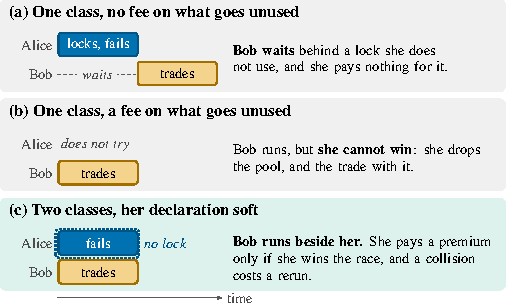
\includegraphics[width=\columnwidth]{figures/fig_alice.pdf}
\caption{Alice's transaction usually finds the price gone, fails and writes nothing, and Bob trades on the same pool. Each panel shows that likely case. In (a) and (b) every declaration takes a lock, the only class of declaration today. She holds it at no charge in (a), and in (b) a fee for unused declarations has made the pool not worth declaring. In (c) the chain offers a second class, soft, which takes no lock (dotted frame).}
\label{fig:alice}
\end{figure}

\runin{An open question}Chains charge very differently for a declaration that goes unused (Table~\ref{tab:chains}). Solana charges nothing for one more declared account, and Sui next to nothing. Stellar charges for every resource a transaction declares, with almost no refund, and Monad charges the whole gas limit whatever is used. A storage key on an Ethereum access list pays for itself only if it is read with probability at least \listThresholdKey{}. In the Object-Weighted Transaction Fee Mechanism (OW-TFM) of Wadhwa et al.~\cite{wadhwa2026perils}, each object has its own price, which rises when the object is used above a target, and a transaction that uses an object pays a usage fee at that price. They show that no fee rule can remove both what a user overpays for unused objects and what the block producer fails to collect on capacity it reserved, unless transactions are executed in advance or the rule is a special case such as a constant fee or one that burns all of the producer's revenue. They propose a fee for each object declared and not used. Their model lists mis-declaration among user actions~\cite[p.~1091]{wadhwa2026perils}, but no theorem treats it, and they leave it open: ``Getting users to reveal their true object sets is an important deployment constraint, and a mechanism that fully enforces it is left to future work''~\cite[pp.~1100--1101]{wadhwa2026perils}. We make this a precise question. Can a fee rule make every transaction declare all it may need and still charge each unused declaration what it costs the chain? The answer is yes exactly when the chain offers some way to leave a declaration unused at no cost (Theorem~\ref{thm:menu}, Proposition~\ref{prop:class} and Theorem~\ref{thm:floor}). Alice's lock is not such a way, since Bob waits behind it whether or not she writes, and a declaration that takes no lock can be. This does not contradict their result, since with a second class each transaction chooses which of the two losses it bears.

\runin{Who holds the locks}On Solana, in transactions other than validators' votes, \notWrittenA\% and \notWrittenB\% of writable declarations other than signers' went unwritten in two samples \sampleGapDays{} days apart. Each transaction also declares a compute limit, and we call the five accounts in a block with the most compute declared on them its hot accounts. Of the time they are locked, transactions that write them hold only \hotWrittenA\% and \hotWrittenB\%. A hundred senders, about 1\% of those active, hold \topHundredUnwrittenA\% and \topHundredUnwrittenB\% of the lock time on them that goes unwritten, and one more writable account adds nothing to what any of them pays. The rule we propose charges a lost race and a deliberate hold alike. When we replay historical blocks as a validator re-executes them on 16 threads, one transaction holding five hot accounts makes the rest of a block take \occFirmFiveA\% and \occFirmFiveB\% longer (Section~\ref{sec:measure} and Appendix~\ref{app:more}).

\runin{What a manipulator can do}A transaction can declare an object it has no use for and hold it against others who need it, under a write lock or a shared one. The block producer, which earns fees, can insert its own transactions, called shills, to raise the prices others pay, and can order transactions so that they do not use what they declared. A transaction can also pay it outside the protocol. A rule for unused declarations decides what each of these costs, and Box~1 states the manipulator model.

\runin{Why one fee is not enough}A transaction that needs an object it did not declare reverts. It fails and pays a revert charge, which cannot exceed the fee its sender signed for. Wadhwa et al.\ expect that charge to stop transactions from leaving objects out~\cite[p.~1100]{wadhwa2026perils}. Yet under a positive fee for each object declared and not used, Alice drops any object she needs rarely enough, since dropping it costs her only an occasional revert. If the fee is zero, every unused lock is paid for by others and anyone can hold an object at no charge. In OW-TFM an unused declaration also raises the price, so the fee must be high enough that a shill does not pay, and that minimum sets how much gets dropped (Section~\ref{sec:oneclass}).

\runin{Two classes}We add one bit to a declaration and call its value the declaration's class. A \emph{firm} declaration takes a lock as today and pays a fee if the object goes unused. A \emph{soft} declaration takes no lock. If another transaction writes the object meanwhile, the transaction runs again, so a soft declaration pays a premium for these reruns when it writes the object. Alice declares the pool soft, and Bob runs beside her. If an unused soft declaration costs the chain nothing, a transaction that can afford the most the rule may charge it loses nothing by declaring all it may need, picks the class that costs the chain less, and pays that class's cost in expectation (Theorem~\ref{thm:menu} and Proposition~\ref{prop:class}). An unused soft declaration is not always free, since the transaction may have read the object, or a validator may have to wait to learn that it did not write it. Every rule with finitely many classes trades dropped objects against unpaid cost, and the class that is cheapest to leave unused sets the terms of that trade. A soft class improves them only by costing less unused than a lock (Theorem~\ref{thm:floor}).

\runin{One rule}We ask four things of a fee rule. Every transaction declares all it may need, each class pays in expectation what it costs the chain, a shill does not pay, and the block producer gains nothing from the added charges by steering a transaction away from what it declared. Suppose an unused soft declaration costs nothing and the price counts only use that was paid for. Then exactly one two-class rule, which we call menu~$M$, meets all four (Theorem~\ref{thm:rule}). Under it an unused firm declaration pays the usage fee it bid times the share of the lock that the chain cannot reclaim after execution, and Alice's soft declaration pays the premium if she writes the pool and nothing otherwise. Every charge beyond the usage fee is burned, and the producer keeps a bounded share of the usage fee. Burning these charges takes nothing from the producer, which earns nothing on an unused lock today. Under this rule a manipulator pays at least the object's price for each unit of capacity it holds under a write lock or a shared one, whatever it bids and however many identities it uses. A producer that inserts the hold gets none of it back (Theorem~\ref{thm:hold}). If a hold keeps the price above its target, its cost grows exponentially with its length (Corollary~\ref{cor:hold}).

\runin{What the classes buy}We replay two samples of Solana blocks and \nPeak{} of its busiest minutes with transactions' behavior fixed (Section~\ref{sec:replay}). Classes set from each sender's public history cut total execution time at 16 threads at a producer free to pick its order by \freeMenuLoCutSixteenA\% and \freeMenuLoCutSixteenB\% when the premium is three times the cost of an unused lock, and by \freeMenuHiCutSixteenA\% and \freeMenuHiCutSixteenB\% at the premium that matches the cost of reruns. Nearly all of the saving comes from freeing locks held by transactions that fail. When transactions adjust their declarations to the fee, charging every unused declaration its full cost loses \frOneLostRA\% and \frOneLostRB\% of fees to reverts with one class and about \frTwoLostRA\% with two (Fig.~\ref{fig:frontier}), the trade-off of Theorem~\ref{thm:floor} on Solana traffic.

\runin{Contributions}\begin{itemize}
\item Measurement: who holds Solana's hot accounts in two samples and \nPeak{} busy minutes, what they cost others and what they pay, how senders on Avalanche responded to a charge on unused gas, and declared objects on Sui, Ethereum and Monad (Section~\ref{sec:measure}).
\item Theory: why no single fee works, the one two-class rule that meets all the goals, and a lower bound on what any hold costs (Sections~\ref{sec:model}--\ref{sec:count}).
\item Evaluation: a replay at a producer and a validator that measures the trade-off of Theorem~\ref{thm:floor} and what a hold costs others, and a reference implementation with a map of the changes to a client (Sections~\ref{sec:replay} and~\ref{sec:prototype}).
\end{itemize}
Theorem~\ref{thm:oneclass} shows why one fee fails. Theorem~\ref{thm:menu}, Proposition~\ref{prop:class} and Theorem~\ref{thm:floor} answer the open question, and Theorems~\ref{thm:rule} and~\ref{thm:hold} give the rule and what a manipulator pays under it. Section~\ref{sec:caps} collects four further results.

\section{Related work}\label{sec:related}

\begin{table}[t]
\centering
\caption{Closest work, what it takes as given, what it gives, and where it sits in our model.}
\label{tab:related}
\footnotesize
\setlength{\tabcolsep}{3pt}
\begin{tabular}{@{}>{\raggedright\arraybackslash}p{0.21\columnwidth}>{\raggedright\arraybackslash}p{0.21\columnwidth}>{\raggedright\arraybackslash}p{0.26\columnwidth}>{\raggedright\arraybackslash}p{0.24\columnwidth}@{}}
\toprule
Work & Takes as given & Gives & In our model \\
\midrule
Wadhwa et al.~\cite{wadhwa2026perils} & Used set inside the declared set & No fee removes both risks; a fee on unused objects; a shill floor & One class, declared-set count, $r^\star_o = \cp_o$ \\
Garimidi; Acilan et al.; Pugatsov et al.~\cite{garimidi2023solana,acilan2025transaction,pugatsov2026execution} & Sets known or supplied & Truthful sets as a goal; gas for parallel work; penalties as a direction & Declarations fixed, or one class \\
Solana proposals~\cite{simd0110,simd0061,eclipse2024solana,simd0553} & Declarations as sent & Write-lock fees, rebates, charges on declared cost; one vote rejected~\cite{sgp0003} & One class; truthfulness not analyzed \\
Chubby~\cite{wei2026chubby} & Inaccurate sets, no fee & Prunes false dependencies at run time, up to 4.64 times the throughput & Leaves who pays and what a fee drops \\
Mostly-optimistic control~\cite{wang2016mostly} & No fee & Read locks where past aborts are many & The replay's classes from history \\
Kiffer et al.; Amores-Sesar et al.; Wang et al.~\cite{kiffer2024nakamoto,amoressesar2026tragedy,wang2026blockspace} & Order before execution; limits given & Deposits or escrow; limits against use; the full reservation charged & Proposition~\ref{prop:caps} with the cap chosen; lower at $\rho > 0$ \\
\bottomrule
\end{tabular}
\end{table}


\runin{Fees under parallel execution}We take the prices of OW-TFM~\cite{wadhwa2026perils} and the one-object setting of its Lemma~4, make the declaration a choice, add a second class of declaration, and change which use counts toward the price; Table~\ref{tab:related} sets the closest work against our model. Diamandis et al.~\cite{diamandis2023designing} update multidimensional prices from observed use, and Section~\ref{sec:count} extends this to capacity that a lock reserves and pays for without using it.

\runin{Measurement}The Solana Foundation~\cite{natale2026resource} and Heimbach~\cite{heimbach2026setting} measure declared against consumed compute and gas, and Heimbach et al.\ measure access-list use and mistakes~\cite{heimbach2025dissecting} and how access sets shift across states~\cite{heimbach2026evm}. Hay et al.~\cite{hay2026analyzing}, who take declared accounts to be accessed, and Anjana et al.~\cite{anjana2025blockchain} analyze Solana's conflict graphs from declared sets, and Tsoi et al.~\cite{tsoi2026not} Sui's from declared write sets. We add whether a declared object was written, by whom, and what fee rules would do on those records.

\runin{Mechanisms with outcome-contingent fees}The probability of use above which declaring an object pays (Section~\ref{sec:oneclass}) is the participation condition of a single refund contract, and our two-class rule is a two-point refund menu in the sense of Courty and Li~\cite{courty2000sequential}, a choice of two contracts that charge differently for non-use. Private failure probabilities with outcome-contingent payment appear in fault-tolerant mechanism design~\cite{porter2008fault} and allocation with penalties for non-use~\cite{ma2019contingent}. In those settings the principal does not move the outcome. Here the block producer can move the outcome through ordering, and the rule of Section~\ref{sec:menu} leaves it nothing to gain from the added charges by doing so.

\section{Declarations on deployed chains}\label{sec:chains}

\begin{table*}[t]
\centering
\caption{What deployed and proposed rules ask for and what they charge, as of November 1, 2026. $\rho$ is the share of unused reserved capacity that can be reclaimed; $\alpha$ is the share of the price charged on the declared cap, and for OW-TFM on an unused object.}
\label{tab:chains}
\footnotesize
\setlength{\tabcolsep}{4pt}
\begin{tabular}{@{}l>{\raggedright\arraybackslash}p{2.8cm}>{\raggedright\arraybackslash}p{4.2cm}>{\raggedright\arraybackslash}p{3.2cm}>{\raggedright\arraybackslash}p{2.5cm}@{}}
\toprule
Rule & Declared in advance & Charge when unused & Reservation & Our result \\
\midrule
Solana~\cite{agave,simd0385} & Accounts, writable flag; compute limit & Object: no fee. Compute: legacy and v0 priority fee on the limit, v1 lump sum & Write lock on each writable account; budgets refilled after execution, on all declared accounts alike & Theorems~\ref{thm:oneclass}(b) and~\ref{thm:hold}; Proposition~\ref{prop:caps} \\
Sui~\cite{suidocs_lfm,suicode} & Input objects, shared ones mutable or read-only & Object: non-refundable storage share only. Compute: as used & Congestion budget advanced on each mutable object before execution & Theorem~\ref{thm:oneclass}(b) \\
Stellar Soroban~\cite{cap0063,stellarfees} & Read-write footprint; resource limits & What is declared, with few refunds & Parallel clusters from the footprint; limits on declared instructions & Theorem~\ref{thm:oneclass}(a) \\
Monad~\cite{monaddocs_gas} & Gas limit; optional access list & Gas limit in full ($\alpha = 1$) & Block space and price on the limit ($\rho = 0$) & Proposition~\ref{prop:caps}: consistent \\
Avalanche C-Chain~\cite{acp194} & Gas limit & $\max\{\text{used}, \text{limit}/2\}$ & Admission on the limit; execution clock and price on the charge & Section~\ref{sec:caps} \\
Ethereum, today~\cite{eip2929,eip2930} & Gas limit; optional access list & Gas as used ($\alpha = 0$); list entry 2,400 or 1,900, and a listed use costs 2,500 or 2,000 less & Producer has executed ($\rho = 1$) & Propositions~\ref{prop:threshold} and~\ref{prop:caps}: $q^\star = \listThresholdAddr$, $\listThresholdKey$ \\
Ethereum, Glamsterdam~\cite{eip8038,eip7981,eip7928} & As above; producer publishes touched sets & List entry 2,900 or 2,000, plus 1,280 or 2,048 of data & As above & Proposition~\ref{prop:threshold}: $q^\star > 1$ \\
OW-TFM~\cite{wadhwa2026perils} (proposed) & Objects, including contingent ones & $\alpha p_o t$ & Declared sets count toward price & Theorems~\ref{thm:oneclass}(c) and~\ref{thm:shill} \\
Menu $M$ (this paper) & Objects, each firm or soft; caps with $\alpha = 1-\rho$ & Firm: $\cp_o$ when unused or read-only. Soft: $k_o$ when used, $u_o$ when unused or read-only & Firm: lock. Soft: none. Price counts what is paid & Theorems~\ref{thm:rule} and~\ref{thm:hold} \\
\bottomrule
\end{tabular}
\end{table*}


\runin{Solana}A transaction lists every account it may touch and marks those it may write. A writable declaration takes a write lock while the transaction runs, whether or not the transaction writes the account~\cite{agave}. The client's cost tracker also keeps a compute budget for the block and one for each writable account, 50 and 20 million units at the current 200~ms slot~\cite{simd0525}. The transaction's estimated cost, computed from its declared compute limit, is charged to the block and to every writable account it declares before it runs. After it runs, the actual cost replaces the estimate on all of those accounts, whether or not each was written, and validators charge the same set when they re-execute the block~\cite{agave}. The fee is a base fee per signature plus a priority fee. In the legacy and v0 formats the priority fee is a price times the declared limit; in the v1 format, active on mainnet since September 2026~\cite{simd0385}, it is a lump sum. Both are due even if the transaction fails, and one more writable account adds nothing to the fee. The reference scheduler of Agave, the main Solana client, ranks transactions by $R/(1+C)$, and that of Firedancer, a second client, by $R/C$, where $R$ is the fee the block producer keeps and $C$ is the estimated cost, including 300 units per write lock~\cite{agave,firedancer}; this is client behavior and not a validity rule, and other schedulers run on mainnet~\cite{simd605}. A 2022 proposal named the gap: ``there is no punishment for taking the write-lock and not using it''~\cite{simd0016}.

\runin{Sui}A transaction lists its input objects and flags each shared one as mutable or read-only; dynamic fields reached through a parent object are not listed~\cite{suidocs_versioning}. Computation is charged on metered units~\cite{suidocs_gas}. Before execution the congestion tracker advances every shared object flagged mutable to the transaction's estimated end time, whether or not execution changes it~\cite{suicode,suidocs_lfm}. The object is written back at a new version even if its contents do not change, and the sender then pays only the non-refundable share of its storage fee, 0.01\% on mainnet~\cite{suicode}: a median of \suiUnchangedFee{} MIST (one MIST is $10^{-9}$ SUI) against a median computation charge of \suiComputationMedian{} MIST in a sample collected in November 2026.

\runin{Stellar}A Soroban transaction declares a read-write footprint and resource limits. The footprint decides which transactions may run in parallel clusters~\cite{cap0063}, and the fee is computed on what is declared, with no refund, apart from a few exceptions, if less is used~\cite{stellarfees}.

\runin{Monad and Avalanche}Monad executes after consensus and charges the gas limit in full, ``rather than the gas used in the course of execution'', and both block space and the base-fee controller count the limit~\cite{monaddocs_gas}. It runs transactions optimistically~\cite{monaddocs_parallel} and requires no object declaration. Avalanche's C-Chain has charged the larger of the gas used and half the limit since September 2026~\cite{acp194,helicon}.

\runin{Ethereum}Gas is charged as used, since the block producer executes before it seals the block. An optional access list prices an entry at 2,400 gas per address and 1,900 per storage key, and a listed entry later costs 100 gas where an unlisted one costs 2,600 or 2,100~\cite{eip2929,eip2930}. The Glamsterdam specification, with no mainnet date as of November 2026~\cite{glamsterdamannounce,glamsterdamdelay}, moves these to 2,900 and 2,000 against 3,000 and 2,100, adds a data charge of 1,280 and 2,048~\cite{eip8038,eip7981}, and has block producers publish the sets actually touched after execution~\cite{eip7928}.
\section{Model}\label{sec:model}

We extend OW-TFM~\cite{wadhwa2026perils} so that a declaration is a choice, and we use the kind of probabilistic model of execution they point to~\cite[p.~1100]{wadhwa2026perils}.

\runin{Prices}Each object $o$ has a posted price $p_o > 0$ per unit of compute, fixed when a transaction is included. A transaction with compute $t$ and priority $\pi \ge 1$ that uses $o$ pays the \emph{usage fee} $\pi p_o t$. The block producer keeps a share $\gamma$ of a fee and the rest is burned. After block $b$ the price moves toward a target use $U^\star_o$ (linearized as in their Lemma~4):
\begin{equation}\label{eq:price}
p_{o,b+1} = p_{o,b}\Bigl(1 + \eta\,\frac{U_{o,b} - U^\star_o}{U^\star_o}\Bigr),
\end{equation}
where $\eta \in (0,1)$ is the responsiveness and $U_{o,b} \ge 0$ is the use counted in block $b$, so prices stay positive. Section~\ref{sec:count} asks what to count.

\runin{Transactions}A transaction's private type is a probability distribution over the set $X$ of objects it will use, with a value $v(X)$ for running with used set $X$. The state it finds at execution decides $X$, and we call each possible $X$ a branch. We write $q_o = \Pr[o \in X]$ for the \emph{probability of use}. For Alice, $X = \{o\}$ if the price is still there and $X = \emptyset$ otherwise, so $q_o$ is her chance of winning the race. A route across two pools has $X = \{A\}$ or $X = \{B\}$. A transaction maximizes its expected value minus fees.

\runin{Declarations}Before it runs, a transaction declares a set $D$ of objects and, under a rule with classes, a class for each. If it needs an object outside $D$, it reverts and pays a revert charge $\kappa \in [0, \bar\kappa]$; the bound holds because a fee cannot exceed what the payer authorized. In the formal model of Wadhwa et al.\ the used set lies inside the declared set by definition~\cite[p.~1090]{wadhwa2026perils}. Letting a transaction leave out what it may need is the step that makes a declaration a choice.

\runin{Classes}A declaration is \emph{firm} or \emph{soft}; we call this its class. A firm declaration locks $o$ for the transaction's running time, as Solana does. A soft declaration takes no lock: the transaction runs beside others, and a collision with another transaction's write to $o$ costs a rerun, as in optimistic execution~\cite{gelashvili2023blockstm}. For a writable declaration we take use to mean a write, which the runtime can observe at commit, so a transaction that fails uses nothing. The two classes waste different things:
\begin{equation*}
\begin{array}{r@{\quad}c@{\quad}c}
 & \text{object used} & \text{object unused}\\
\text{firm} & 0 & (1-\rho)\,c_o\\
\text{soft} & k_o & r_o
\end{array}
\end{equation*}
Here $c_o = \pi p_o t$ is what the transaction bid for the object's capacity over its running time, $\rho \in [0,1]$ is the share of an unused lock's capacity that can be reclaimed after execution, and we write $\cp_o = (1-\rho) c_o$. The cost $k_o$ is the expected cost of reruns per use, its own and those it causes others, posted with the price (Proposition~\ref{prop:premium} treats how). The cost $r_o \ge 0$ of an unused soft declaration is zero if the transaction does not read what it does not use and nobody has to wait to learn this. It is positive if the transaction read $o$, so that a write to $o$ makes it run again, or if a validator that re-executes in block order cannot commit a later declarer of $o$ until it learns that the transaction did not write $o$. Section~\ref{sec:replay} measures it. If $r_o \ge \cp_o$ a lock is cheaper at every probability of use, so we take $r_o \le \cp_o$ and write $\qL = (\cp_o - r_o)/(\cp_o - r_o + k_o)$ for the probability of use above which a lock costs less, taking $k_o > 0$ if $r_o = \cp_o$. A read-only declaration has the same two classes. A firm one takes a shared lock, so writers wait for it. A soft one takes no lock and is checked at commit, so a write to the object during its run makes the transaction run again. The runtime does not see reads, so it cannot tell whether either was used, and the check at commit can run over everything declared.

\runin{Fee rules}A \emph{one-class rule} gives every declaration the same class and charges, on top of the usage fee, a fee $f_n$ if the object goes unused. OW-TFM charges an unused object $f_n = \alpha p_o t$, a fraction $\alpha$ of the object's price per unit of compute. A \emph{two-class rule} lets the transaction pick a class for each object and charges each class its own fees.

\noindent\fbox{\parbox{\dimexpr\columnwidth-2\fboxsep-2\fboxrule\relax}{
\textbf{Box 1. Manipulator model.}
\emph{Declarers.} A transaction may omit objects, declare objects it does not expect to use, and pick any class, writable or read-only. It knows its own distribution of $X$ and the posted terms. A manipulator may declare an object only to hold capacity that others need. It may use any number of identities and pay part of its bid outside the protocol, posting a priority as low as $\pi = 1$.
\emph{Block producer.} It may insert its own transactions (\emph{shills}) to raise later prices~\cite{wadhwa2026perils}; a shill pays fees like any transaction and the producer gets back its share of them. It may order transactions to steer which branch each takes, and run transactions with soft declarations last. It learns a transaction's branch only by running it. It may take payments outside the protocol and act with the payers as one party.
\emph{Outside the model.} A producer that excludes transactions, as in~\cite{wadhwa2026perils}; consensus, which is honest. Prices, $\rho$ and running times are given, a transaction's type is its own, and the only equilibrium we treat is how much soft use a posted premium draws.}}
\smallskip

\runin{Goals}Let $F(X)$ be the most a rule can charge when $X$ occurs. A branch with $v(X) + \kappa < F(X)$ is rightly dropped, so the first goal below asks only about types that can afford every branch, those with $v(X) + \kappa \ge F(X)$ for every used set $X$ in their support.

\begin{definition}\label{def:goals}
A fee rule has
\begin{itemize}
\item \emph{complete declaration} if every type that can afford every branch has a best response that declares every object with $q_o > 0$;
\item \emph{cost matching} if, for each class and every $q_o$, the expected fee beyond the usage fee equals the expected cost of a declaration of that class;
\item \emph{shill resistance} if no shill raises the producer's revenue over the next $\Lambda \ge 1$ blocks it produces by more than the shill burns;
\item \emph{ordering neutrality} if the producer keeps at least as much of the charges beyond the usage fee when a transaction uses a declared object as when it takes a branch that leaves the object unused.
\end{itemize}
\end{definition}

In Fig.~\ref{fig:alice} the first two goals pull apart under one class, since in (b) a fee on Alice's unused lock makes her drop the pool and in (a) no fee leaves the lock's cost on Bob. We also track two properties that are not goals: in a complete best response each writable object takes the class with the lower expected cost, $\min\{(1-q_o)\cp_o,\ q_o k_o + (1-q_o) r_o\}$, and a declaration that is unused or read-only pays what it costs the chain, which for a lock is $\pi p_o$ per unit of capacity held.

\section{Why one fee fails}\label{sec:oneclass}

Take an object $o$ with probability of use $q$, and let $x$ be the net value of the branch that uses it, the branch's value minus its fees.

\begin{lemma}[Declaration threshold]\label{prop:threshold}
Under a one-class rule, declaring $o$ beats omitting it if and only if $q(x+\kappa) \ge (1-q) f_n$, which for $f_n + x + \kappa > 0$ reads $q \ge q^\star(f_n) = f_n/(f_n + x + \kappa)$.
\end{lemma}

\begin{proof}
Declaring gains $x + \kappa$ on the branch that uses $o$ and costs $f_n$ on the other.
\end{proof}

Ethereum's access lists are an instance. There an omitted entry costs the cold price (the price of a first access) with no revert, so the threshold depends only on what a listed entry saves when it is used. At current prices an address pays for itself only if it is used with probability at least \listThresholdAddr{}, and a storage key only if it is used with probability at least \listThresholdKey{} when first read and \listThresholdKeyWrite{} when first written. Under the Glamsterdam prices listing an address saves nothing, nor does listing a storage key that is first read, and with the data charge a list loses gas at every probability of use.

\begin{theorem}[Limits of one class]\label{thm:oneclass}
Consider a one-class rule, with $\kappa \le \bar\kappa$, $x + \bar\kappa > 0$ and types with arbitrarily small $q > 0$. If $f_n > 0$, every object with $q < f_n/(f_n + x + \bar\kappa)$ is omitted, so complete declaration holds for all types only if $f_n = 0$.
\end{theorem}

\begin{proof}
This follows from Lemma~\ref{prop:threshold}, since the threshold falls in $\kappa$.
\end{proof}

With $f_n = 0$ and firm declarations, each declaration instead leaves the expected cost $(1-q)\cp_o$ of Section~\ref{sec:model} unpaid, and a manipulator can hold capacity at no charge for the object. A chain therefore either charges a positive fee and loses rarely used objects, as Stellar and Ethereum's lists do, or charges nothing and leaves unused locks unpaid, as Solana and Sui do.

\begin{proposition}[Shills under one class]\label{prop:oneshill}
Under the rule of Theorem~\ref{thm:oneclass} with prices that count declared sets and $\gamma < 1$, shill resistance requires $\alpha \ge \alpha_{\min} = \Lambda \pi_o \eta \gamma/(1-\gamma)$, where $\pi_o$ is the average priority on $o$ ($\Lambda = 1$ in~\cite[Lemma~4]{wadhwa2026perils}). With $f_n = \alpha p_o t$, every object with $q < \alpha_{\min} p_o t/(\alpha_{\min} p_o t + x + \bar\kappa)$ is then omitted, and if $\alpha_{\min} > 1$ no $\alpha \le 1$ resists shills.
\end{proposition}

\begin{proof}
The bound $\alpha_{\min}$ equates the burn $(1-\gamma)\alpha p_o$ of a declared unit with the $\Lambda\gamma\eta\pi_o p_o$ it brings back, and Lemma~\ref{prop:threshold} gives the drops.
\end{proof}

Lemma~4 of Wadhwa et al.\ takes $\eta = 1/8$, $\gamma = 1/2$ and $\Lambda = 1$. There $\alpha_{\min}$ is 2 at the 95th-percentile priority of 16 they use, so no $\alpha \le 1$ resists shills, and $5/8$ at their mean priority of 5, so Proposition~\ref{prop:oneshill} drops every object used rarely enough.

\begin{figure}[t]
\centering
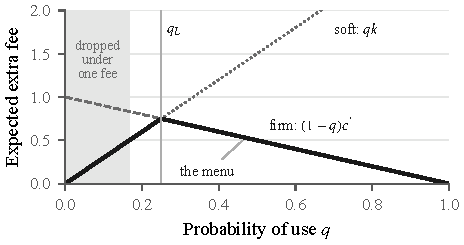
\includegraphics[width=\columnwidth]{figures/fig_costs.pdf}
\caption{Expected fee beyond the usage fee, against the probability of use, with $\cp_o = 1$, $k_o = 3$ and $r_o = 0$, so $\qL = 1/4$. The solid line is what the two-class rule $M$ of Section~\ref{sec:menu} charges. Objects whose $q$ falls in the shaded range are dropped under a one-class fee $f_n = 1$ when $x + \kappa = 5$, so $q^\star = 1/6$.}
\label{fig:costs}
\end{figure}

\section{Two classes}\label{sec:menu}

One class cannot fit every probability of use. If $r_o < \cp_o$ and $k_o > 0$, firm costs more than soft for $q < \qL$ and soft more than firm for $q > \qL$, since $(1-q)\cp_o$ falls in $q$ faster than $q k_o + (1-q) r_o$ and the two cross at $\qL \in (0,1)$. A second class lets each object take the cheaper one.

\begin{definition}[Menu $M$]\label{def:menu}
Each declaration is firm or soft. A firm declaration pays the usage fee if the object is used and $\cp_o$ if it is not. A soft declaration pays the usage fee plus the premium $k_o$ if the object is used and a charge $u_o \in [0, r_o]$ if it is not. A read-only declaration cannot show use: it pays $\cp_o$ if firm and $u_o$ if soft. Everything beyond the usage fee is burned, and the producer keeps $\gamma$ of the usage fee.
\end{definition}

The menu is outside the family of Wadhwa et al., who require that declaring uncertainty never cost more than declaring certainty~\cite[Section~3]{wadhwa2026perils}: a used soft object pays more than a used firm one. That departure lets a rarely used object go soft, so the fee on unused objects only has to price a held lock. With $\rho < 1$ a firm object left unused still pays above the usage fee, one of the two risks of their Theorem~1. Each transaction now chooses which risk it bears. A used set's highest fee $F(X)$ adds $\pi p_o t + k_o$ for each writable object in $X$ and $\cp_o$ for every other object the type may use.

\begin{theorem}[The menu]\label{thm:menu}
Under menu $M$, a type that declares every other object it may use prefers declaring $o$ soft to omitting it if and only if $q_o (x_o + \kappa) \ge (1-q_o) u_o$, where $x_o$ is the expected net value of the branches that use $o$. So at $u_o = 0$ every type that can afford every branch has a complete best response, one that declares every object with $q_o > 0$, and if each margin $v(X) + \kappa - F(X)$ is positive, every best response is complete.
\end{theorem}

\begin{proposition}[Classes under the menu]\label{prop:class}
In a complete declaration under $M$, a writable object with $q_o > (\cp_o - u_o)/(\cp_o - u_o + k_o)$ is firm and one below it is soft, so its expected fee beyond the usage fee is $\min\{(1-q_o)\cp_o,\ q_o k_o + (1-q_o) u_o\}$. At $u_o = r_o$ the threshold is $\qL$ and this fee is the expected cost of the cheaper class. At $u_o < r_o$ a soft object leaves $(1-q_o)(r_o - u_o)$ unpaid.
\end{proposition}

The proof (Appendix~\ref{app:proofs}) separates the payoff of a complete declaration into a term the classes cannot affect and one cost per object, so each object's class is decided alone for any joint distribution of use, and given the posted terms nothing depends on what others declare. Take Alice with $q_o = 0.05$, $\cp_o = 1$, $k_o = 3$ and $x + \kappa = 5$, the values of Fig.~\ref{fig:costs}. Under the one-class fee $f_n = 1$ she drops the pool and loses $0.25$ in expectation to reverts. With no fee she declares it, pays nothing, and leaves a lock whose expected cost of $0.95$ falls on others. Under the menu with $r_o = 0$ she pays $0.15$, and Bob runs beside her. A read-only declaration pays $\cp_o$ firm and $u_o \le \cp_o$ soft whatever the branch, so at $u_o = 0$ a soft read gains $q_o(x_o + \kappa)$ against omitting the object and none is dropped, and only a manipulator that declares an object just to hold it has a reason to take a shared lock.

\begin{corollary}\label{cor:between}
\textup{(a)} At $u_o = r_o$ the total expected cost of a complete declaration under $M$ is at most the smaller of all-firm and all-soft, and strictly less when writable objects lie on both sides of $\qL$. \textup{(b)} At $u_o = 0$ a transaction that can afford every branch and uses exactly one of several pools, with probabilities $q_j$, has a best response that declares all of them and pays $\sum_j \min\{(1-q_j)\cp_j,\ q_j k_j\}$ beyond the usage fee.
\end{corollary}

Part (b) is the routing case that Wadhwa et al.\ leave out of scope~\cite[p.~1090]{wadhwa2026perils}, where a rule with $f_n > 0$ would charge for every pool left unused.

A producer that orders transactions can change which branch a transaction takes, so a fee that pays it more for an unused object than for a used one would reward it for steering them. Wadhwa et al.\ note this and ask that the retained share rise with use, then take $\gamma$ constant~\cite[p.~1091]{wadhwa2026perils}. Let $\sigma \in [0,1]$ be the share of capacity left free that the producer can resell at the price $p_o$. Neutrality asks this of what a rule adds to the usage fee, since the usage fee and resale are there under any rule.

\begin{lemma}[Ordering neutrality]\label{prop:neutral}
\textup{(a)} Menu $M$ is ordering neutral, since it burns what it adds to the usage fee. With the usage fee and resale the producer keeps at least as much on an object when it is used: $\gamma \pi p_o t$ against $\gamma\sigma\rho p_o t$ on a firm object and $\gamma\sigma p_o t$ on a soft one. \textup{(b)} Let $\rho < 1$ and $k_o > 0$, and let a transaction declare $A$ firm and $B$ soft at equal prices $p_o$ and use exactly one of them, and let the producer keep shares $\gamma'$ of the fee on unused firm objects and $\gamma_k$ of the premium. It can resell all of $B$'s capacity when the transaction takes $A$, since a soft object holds none, and the reclaimed share $\rho$ of $A$'s when the transaction takes $B$. Counting this, it earns $(1-\rho) p_o t (\gamma'\pi - \gamma\sigma) + \gamma_k k_o$ more when the transaction takes $B$. Of this, $\gamma'\cp_o + \gamma_k k_o$ comes from what the rule adds, so the rule rewards steering toward $B$ unless $\gamma' = \gamma_k = 0$, and under $M$ the producer gains $\gamma\sigma(1-\rho)p_o t$ by steering toward $A$.
\end{lemma}

Part (b) is why $M$ burns what it adds. Neutrality also places the menu among scoring rules. If a transaction instead reported a probability $\hat q$ and paid $J(\hat q) + J'(\hat q)(y - \hat q)$ beyond the usage fee, with $y$ the indicator of use and $J$ concave with supergradient $J'$, a producer keeping a share $\gamma_J$ would get $\gamma_J J'(\hat q)$ more when the object is used, so the rule is neutral exactly when $\gamma_J J'(\hat q) \ge 0$ for every report. The menu at $u_o = 0$ is this payment for $J(q) = \min\{(1-q)\cp_o,\ q k_o\}$, the proper scoring rule of a kinked cost~\cite{gneiting2007strictly}, so a transaction only has to land on the right side of the kink. A premium charged on realized conflicts and kept by the producer would reward it for causing them; one charged on use and burned does not depend on the order.

\runin{What a second class buys}Let $r^\star_o$ be the least expected cost of an unused declaration of $o$ among the classes a chain offers: $\cp_o$ with locks alone, $r_o$ with soft declarations.

\begin{theorem}[The trade-off]\label{thm:floor}
Let a fee rule have finitely many classes, and let $x$, with $x + \bar\kappa > 0$, be the largest net value of the branches that use $o$ across its classes. A rule with no drops leaves at least $r^\star_o$ unpaid on an unused declaration in some class, and a rule under which every unused declaration pays its cost drops objects below $q = r^\star_o/(r^\star_o + x + \bar\kappa)$.
\end{theorem}

\begin{proof}
Let $u$ be a lower bound on what the rule charges an unused declaration of $o$ in any class. A type that declares every other object it may use then drops $o$ whenever $q_o < u/(u + x + \bar\kappa)$, because in any class with charge $a \ge u$ on non-use, declaring gains at most $q_o(x + \bar\kappa)$ against omitting, on the branches that use $o$, and costs $(1-q_o) a \ge (1-q_o) u$ on the others. A declaration in a class that charges exactly $u$ leaves at least $r^\star_o - u$ unpaid when it goes unused, since it then costs at least $r^\star_o$. We now take $u$ to be the least charge, which some class makes since there are finitely many. A rule with no drops needs $u = 0$, since otherwise a type with small enough $q_o$ drops $o$, and then that class leaves at least $r^\star_o$ unpaid. If every unused declaration pays its cost, every charge is at least $r^\star_o$, and the first step applies with $u = r^\star_o$.
\end{proof}

A one-class rule with locks has $r^\star_o = \cp_o$, which is Theorem~\ref{thm:oneclass} and the zero fee after it. Menu $M$ has $r^\star_o = r_o$ and attains this bound at $u_o = 0$; at $u_o > 0$ its threshold in Table~\ref{tab:compare} can be higher, since a used soft object also pays the premium. So what a second class buys is the fall of $r^\star_o$ from $\cp_o$ to $r_o$. At $r_o = 0$ complete declaration and cost matching hold together. At $r_o = \cp_o$ the second class changes nothing in this trade-off. Fig.~\ref{fig:frontier} draws it on Solana traffic. The same holds for reads. Shared locks alone are one class, and a charge on them drops what is rarely read; a soft read lowers $r^\star_o$ to what its own reruns cost, and it needs no sight of reads, since a firm read pays for its lock and a soft one is checked over all it declared.

\section{What counts toward the price}\label{sec:count}

The utilization formula of Wadhwa et al.\ sums $t$ over the transactions that declare an object, so in their Lemma~4 a shill adds its full $t$ to the count while it pays $\alpha p_o t$. Their text notes that a transaction that under-executes could count for less~\cite[p.~1099]{wadhwa2026perils}, and we take that route. Under declared-set counting the fee on unused objects has to deter shills as well as price declarations.

\begin{definition}[Count what is paid]\label{def:count}
$U_{o,b}$ counts a transaction's use of $o$ as $t$ if it used $o$, as $(1-\rho)t$ if it held a lock on $o$ and did not write it, and as $0$ otherwise.
\end{definition}

Counting what is paid is not new for gas limits: Avalanche's rule of Section~\ref{sec:chains} and Monad move their prices by the gas they charge~\cite{acp194,monaddocs_gas}. Under menu $M$ every counted unit pays $\pi p_o$, used or not.

\begin{proposition}[Shills]\label{thm:shill}
In the setting of Lemma~4 of~\cite{wadhwa2026perils} (one object, the linearized update~\eqref{eq:price}), let every block after the one with a shill have honest use at the target, with average priority $\pi_o$ in the next $\Lambda$ blocks made by the producer that inserted the shill. Under menu $M$ with prices that count what is paid, no shill of any size, class, priority or use is profitable if and only if
\begin{equation}\label{eq:shill}
\gamma \le \frac{1}{1 + \eta \pi_o \Lambda}.
\end{equation}
\end{proposition}

The condition does not involve $\rho$, $k_o$ or any fee on unused objects. Under declared-set counting the condition is $(1-\gamma)\alpha \ge \gamma \eta \pi_o \Lambda$ (Proposition~\ref{prop:oneshill}), which at $\alpha = 1$ is~\eqref{eq:shill}. So counting what is paid gives every declaration the shill resistance that declared-set counting reaches only by charging unused objects in full. The burned share needed rises with $\pi_o \Lambda$: at $\eta = 1/8$ a burned share of $1/2$ covers $\pi_o \Lambda$ up to 8, and 16 needs $2/3$. On Solana one producer makes four consecutive slots~\cite{simd0525}, so a shill in the first has $\Lambda \ge 3$.

The goals together leave one rule. Consider a two-class rule whose prices count what is paid. Beyond the usage fee it charges a writable firm declaration $a_1$ if the object is used and $a_0$ if it is not, and a soft one $\tilde a_1$ and $\tilde a_0$, and the producer keeps shares $\gamma$ of the usage fee, $\gamma'$ of $a_0$ and $\gamma_k$ of $\tilde a_1$.

\begin{theorem}[The rule]\label{thm:rule}
Let $r_o = 0$, $\rho < 1$ and $k_o > 0$. Such a rule has cost matching, complete declaration, ordering neutrality and shill resistance in the setting of Proposition~\ref{thm:shill} if and only if it is $M$ with $u_o = 0$ and $\gamma \le 1/(1 + \eta\pi_o\Lambda)$, that is, $a_1 = \tilde a_0 = 0$, $a_0 = \cp_o$, $\tilde a_1 = k_o$ and $\gamma' = \gamma_k = 0$.
\end{theorem}

\begin{proof}
Cost matching says $q a_1 + (1-q) a_0 = (1-q)\cp_o$ and $q \tilde a_1 + (1-q) \tilde a_0 = q k_o$ for all $q$, and $q = 0$ and $q = 1$ give the four fees. Lemma~\ref{prop:neutral}(b) gives $\gamma' = \gamma_k = 0$, and Proposition~\ref{thm:shill} gives the bound on $\gamma$. Conversely, at $u_o = r_o = 0$ Theorem~\ref{thm:menu} gives complete declaration and Proposition~\ref{prop:class} cost matching, Lemma~\ref{prop:neutral}(a) gives neutrality, and Proposition~\ref{thm:shill} gives shill resistance.
\end{proof}

By Proposition~\ref{prop:class} each writable object then takes the cheaper class, and by Definition~\ref{def:menu} every unused or read-only declaration pays what it costs the chain. If $r_o > 0$, cost matching gives $\tilde a_0 = r_o$ and complete declaration fails below the threshold of Theorem~\ref{thm:floor}, and the rest stands. Cost matching also sets the fees on reads, $\cp_o$ on a firm one and $u_o$ on a soft one, and it is what a manipulator faces next.

\begin{theorem}[The price of holding]\label{thm:hold}
Let a manipulator's locks hold $H_o$ of an object's capacity in a block, the sum of $(1-\rho)t$ over its firm declarations that it does not use and its firm read-only ones, under any number of identities and at any priorities. Under $M$ it pays at least $p_o H_o$ for them, and a producer that inserts them gets none of it back.
\end{theorem}

\begin{proof}
Each such declaration pays $(1-\rho)\pi p_o t \ge p_o (1-\rho) t$, the sum runs over declarations and not identities, and all of it is burned.
\end{proof}

\begin{corollary}\label{cor:hold}
Let the manipulator hold $H_o > 0$ in each of $T$ blocks from the price $p_o$, and let the count stay at or above $(1+g)U^\star_o$ with $g > 0$, as it does with $g = H_o/U^\star_o$ if other use stays at the target. When prices count what is paid, it pays at least
\begin{equation}\label{eq:hold}
P(T) = p_o H_o\, \frac{(1 + \eta g)^T - 1}{\eta g},
\end{equation}
so spending $S$ buys at most $\log(1 + S\eta g/(p_o H_o))/\log(1 + \eta g)$ blocks.
\end{corollary}

\begin{proof}
By~\eqref{eq:price} the count gives $p_{o,b} \ge p_o (1+\eta g)^b$, and by Theorem~\ref{thm:hold} block $b$ pays at least $p_{o,b} H_o$. Summing over $b < T$ gives~\eqref{eq:hold}.
\end{proof}

An unused soft declaration or a soft read holds no lock and writes nothing. What it can add to others' waiting is a thread for its reruns and, if it is writable, a wait at a validator not told what was written; $r_o$ counts both, and at $u_o = r_o$ it pays for them in expectation. A one-class fee $f_n$ prices a held lock at $f_n/((1-\rho)t)$ per unit, below $\pi p_o$ whenever $f_n < \cp_o$; on Solana today it is zero. If others leave as the price rises, a price at which their demand equals $U^\star_o - H_o$ is stationary, and a hold that reaches it pays it for as long as it lasts.

Table~\ref{tab:compare} sets the rules against the goals of Section~\ref{sec:model}, and Section~\ref{sec:replay} measures $r_o$ and what a hold costs.

\begin{table*}[t]
\centering
\caption{Rules against the goals of Section~\ref{sec:model}.}
\label{tab:compare}
\footnotesize
\setlength{\tabcolsep}{4pt}
\begin{tabular}{@{}lccccll@{}}
\toprule
Rule & \begin{tabular}{@{}c@{}}Lowest $q$\\declared\end{tabular} & \begin{tabular}{@{}c@{}}Cheaper\\class\end{tabular} & \begin{tabular}{@{}c@{}}Cost\\matching\end{tabular} & \begin{tabular}{@{}c@{}}Unused\\pays cost\end{tabular} & \begin{tabular}{@{}l@{}}Ordering\\neutrality\end{tabular} & \begin{tabular}{@{}l@{}}Shill resistance\end{tabular} \\
\midrule
One class, no fee (Solana, Sui) & 0 & no & no & no & yes & no object prices \\
One class, $f_n = \alpha p_o t$ (OW-TFM) & $\phi(f_n)$ & no & at $f_n = \cp_o$ & at $f_n = \cp_o$ & if $f_n$ is burned & $(1-\gamma)\alpha \ge \gamma\eta\pi_o\Lambda$ \\
All soft, premium on use, charge $u_o$ & $\phi_k(u_o)$ & no & at $u_o = r_o$ & at $u_o = r_o$ & yes & $\gamma \le 1/(1+\eta\pi_o\Lambda)$ \\
Menu $M$ & \begin{tabular}{@{}c@{}}$\min\{\phi(\cp_o),$\\$\phi_k(u_o)\}$\end{tabular} & at $u_o = r_o$ & at $u_o = r_o$ & \begin{tabular}{@{}c@{}}locks; soft at\\$u_o = r_o$\end{tabular} & yes & $\gamma \le 1/(1+\eta\pi_o\Lambda)$ \\
\bottomrule
\end{tabular}
\par\smallskip\parbox{\textwidth}{\scriptsize Lowest $q$ declared: the lowest probability of use at which an object is declared, with $\phi(u) = u/(u + x + \bar\kappa)$ for a charge $u$ on non-use and $\phi_k$ the same with $x - k_o$ in place of $x$, for $x - k_o + \bar\kappa > 0$; by the proof of Theorem~\ref{thm:floor} no rule falls below $\phi$ of its least charge. The last column is for the setting of Proposition~\ref{thm:shill}; in the last two rows prices count what is paid. The rows cover writable declarations, and in the last row the column Unused pays cost covers shared locks as well. Sui's dynamic fields are not declared at all (Section~\ref{sec:chains}).}
\end{table*}


\section{Extensions}\label{sec:caps}

The premium is a posted estimate of a cost that depends on how many transactions choose soft, and that choice depends on the premium. Take $u_o = r_o = 0$. Let the declarers of an object have a joint distribution $G$ of $(q, \cp)$ with $\cp > 0$ and no atom on the curves $q = \cp/(\cp + k)$, let $s(k) = \int q\,\mathbf{1}\{q < \cp/(\cp + k)\}\,dG$ be the soft use at premium $k$, and let $\psi(s)$ be the realized cost per use at soft use $s$, continuous and nondecreasing. Write $\Psi(k) = \psi(s(k))$.

\begin{proposition}[Posting the premium]\label{prop:premium}
\textup{(a)} There is exactly one stationary premium $k^\star = \Psi(k^\star)$. \textup{(b)} Posting last block's cost, $k_{b+1} = \Psi(k_b)$, need not converge: for uniform $q$, $\cp = 1$ and $\psi(s) = 36 s$ we have $k^\star = 2$ and $\Psi'(k^\star) = -4/3$. \textup{(c)} If $\Psi$ is $\lambda$-Lipschitz, the damped update $k_{b+1} = (1-\delta)k_b + \delta \Psi(k_b)$ converges to $k^\star$ from any start for $\delta \in (0,1]$ with $\delta < 2/(1+\lambda)$.
\end{proposition}

So a chain should move the premium in small steps, as EIP-1559 moves the base fee~\cite{roughgarden2024transaction}.

\begin{proposition}[Running soft declarations last]\label{prop:place}
Let a producer bear the reruns it schedules, an expected $k_o$ per use if a soft declaration runs at its rank and none if it runs after every transaction that conflicts with it. Let $q$ be the probability of use at its rank and $q' \le q$ after them, let the producer keep a share $\gamma_k$ of the premium, and for a transaction that may use only $o$ let $V = v(\{o\}) - \pi p_o t - v(\emptyset)$. \textup{(a)} Running it at its rank rather than last gains the producer $(q - q')(\gamma(\pi - \sigma) p_o t + \gamma_k k_o) - q k_o$. If $q' = q$ this is $-q k_o$ for every $\gamma_k$, since a premium charged on use is paid either way. \textup{(b)} Against a producer that places it last, such a transaction prefers firm to soft if and only if $(q - q')V + q' k_o + (1 - q') u_o \ge (1 - q)\cp_o$. At $q' = q$ this is the comparison of Proposition~\ref{prop:class}. At $q' = 0$ and $u_o = 0$ it reads $qV \ge (1-q)\cp_o$, which is Lemma~\ref{prop:threshold} at $f_n = \cp_o$ with $V$ in place of $x + \kappa$.
\end{proposition}

So a route, whose use does not depend on position, keeps the second class, and a racer that wins only by running early keeps its rank only if the producer's share of its fee covers the reruns it causes, and otherwise pays the producer, pays for a lock or stops trying.

\begin{proposition}[Transfers]\label{prop:transfers}
Let transactions and the producer act as one party with any transfers among them, and let a transaction with bid $\pi$ post $\pi' \in [1, \pi]$ and pay the rest by transfer. Under menu $M$:
\textup{(a)} A unit of capacity burns $\pi' p_o \ge p_o$ under a lock that goes unused or is read-only, and $(1-\gamma)\pi' p_o$ of the usage fee if the party writes the object, plus the premium on a soft one.
\textup{(b)} Apart from the producer's resale and reruns, the party treats it as a lone transaction that posts $\pi'$, values $X$ at $v(X) + \gamma \sum_{o \in X \text{ writable}} \pi' p_o t$ and has revert charge $(1-\gamma_{\mathrm{rev}})\kappa$ when the producer keeps a share $\gamma_{\mathrm{rev}}$ of a revert charge, so Theorem~\ref{thm:menu} and Proposition~\ref{prop:class} hold for it.
\textup{(c)} With the terms of Proposition~\ref{prop:place} and a producer that bears reruns, the party prefers running a transaction with a soft declaration at its rank to running it last if and only if $(q-q')(V - k_o + u_o + \gamma(\pi'-\sigma)p_o t) \ge q k_o$, which at $q' = 0 < q$ reads $V + u_o + \gamma(\pi'-\sigma)p_o t \ge 2k_o$.
\end{proposition}

So at a given posted bid a transfer buys neither a cheaper class nor a cheaper lock, since what the rule adds is burned whoever pays it, and it can lower the posted bid no further than $\pi' = 1$.

A gas or compute limit is a declaration too. A transaction needs $Z \sim Q$ units, sets a limit $d$, succeeds if $Z \le d$ for a value $v$, and consumes $\min\{Z, d\}$. The chain reserves $d$ and recovers a share $\rho$ of what goes unused. With $\chi$ the cost of a unit of capacity, the efficient limit maximizes
\begin{equation}\label{eq:capS}
W(d) = v Q(d) - \chi\bigl[(1-\rho) d + \rho\,\mathbb{E}\min\{Z,d\}\bigr].
\end{equation}
A linear rule charges a share $\xi$ of the price $p$ on the limit and the rest on use, so the user maximizes
\begin{equation}\label{eq:capU}
\Pi(d) = v Q(d) - p\bigl[\xi d + (1-\xi)\mathbb{E}\min\{Z,d\}\bigr].
\end{equation}

\begin{proposition}[Limit charge]\label{prop:caps}
Let $p, \chi > 0$. For every $Q$ and $v$ the user's optimal limits are the efficient ones if and only if $p = \chi$ and $\xi = 1 - \rho$.
\end{proposition}

Monad charges the whole limit and counts it ($\xi = 1$, $\rho = 0$), and Ethereum charges use after the producer has executed ($\xi = 0$, $\rho = 1$), so their rules look opposite and follow one formula.

\section{What is declared and what is used}\label{sec:measure}

\runin{Data}We took two samples of Solana: Sample A (October 2026) and Sample B (October and November 2026), each \nBlocksA{} blocks spaced 1,800 slots apart, with \nTxA{} and \nTxB{} non-vote transactions, that is, transactions other than validators' votes. Both run under the 200~ms slot parameters, and Alpenglow, Solana's new consensus protocol~\cite{simd0326}, activated between them in October 2026. We also took whole minutes of consecutive blocks, 300 slots each, from a public node's records of \winRecordHours{} hours over two days in November 2026: the \nPeak{} busiest, at \winTpsLo{} to \winTpsHi{} non-vote transactions per second against medians of \winTpsMedianOne{} and \winTpsMedianTwo{} on the two days, and the \nMedian{} minutes closest to the second day's median, with \nMinuteBlocks{} blocks and \nMinuteTx{} transactions in all. Appendix~\ref{app:methods} gives the sampling and the definitions, and Tables~\ref{tab:measure} and~\ref{tab:windows} in Appendix~\ref{app:more} collect the results.

\runin{Which accounts were written}Solana's block metadata does not say which accounts a transaction wrote, so we infer writes. A failed transaction wrote nothing beyond its fee payer and any durable nonce account it advances (an account that keeps a signed transaction valid until it is sent), since its other changes are rolled back; our records do not identify nonce accounts, so they count as unwritten. A token account whose balance did not change counts as unwritten, and so does an account that only a router's untaken leg referenced. Every other account counts as written, including all data writes we cannot see. Under these rules \notWrittenA\% and \notWrittenB\% of declarations of writable non-signer accounts went unwritten, \notWrittenOkA\% and \notWrittenOkB\% within successful transactions. Fig.~\ref{fig:declared}(a) shows the share rising with how often an object was declared.

\begin{figure*}[t]
\centering
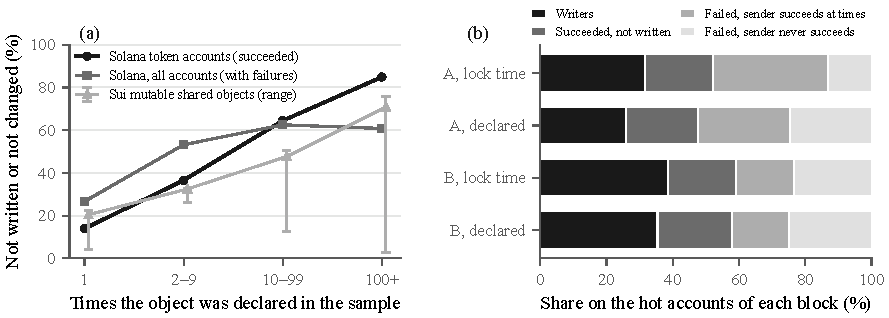
\includegraphics[width=\textwidth]{figures/fig_declared.pdf}
\caption{(a) Share of declared writable objects not written (for Sui, not changed), by how often the object was declared in the sample. Solana token accounts count successful transactions only; the Sui bars run from the strict lower bound to the upper bound of Appendix~\ref{app:methods}, with the marker at the middle estimate. Sample A for Solana. (b) Who holds the five accounts with the most declared compute in each block, as a share of the lock time (consumed compute) and of the compute declared on them. The last segment includes senders seen once or twice.}
\label{fig:declared}
\end{figure*}

\runin{Who holds the hot accounts}In each block we take the five accounts with the most declared compute and split the time locks on them were held by who held them (Fig.~\ref{fig:declared}(b)). Transactions that write the account hold \hotWrittenA\% and \hotWrittenB\% of it, and \winHotWrittenMin\% to \winHotWrittenMax\% in the busiest minutes. Most of the rest is failed transactions, and senders with no success in the whole sample hold \hotNeverA\% and \hotNeverB\%. Holding is concentrated: the 100 senders with the most unwritten lock time, of \nSendersA{} and \nSendersB{}, have \topHundredUnwrittenA\% and \topHundredUnwrittenB\% of it. The client charges a transaction's cost to every writable account it declares, so non-writers also take these accounts' budgets, yet the budget sits far above use: after execution the charge on a hot account has a median of \usedLimMedA\% and \usedLimMedB\% of the 20-million budget, and \winUsedLimMedMin\% to \winUsedLimMedMax\% in the busiest minutes.

\runin{Lost races or holds}Public data cannot show intent. Holders do not sit early in the block, those that never succeeded pay less priority fee than writers (Table~\ref{tab:measure}), and only \sameBlockA\% and \sameBlockB\% of unwritten lock time comes from senders that write the same account in the same block. So what we see looks like races lost, and what a holder costs others does not depend on what it meant.

\runin{Who declares what}In the data of Zheng et al.~\cite{zheng2025why} the largest cause of failure is a price or profit check not met, at 47.99\%, so many failed transactions read the state to find that they have lost. Many declarations look predictable from the sender's own record: pairs of sender and account seen at least three times cover \pairCoverA\% and \pairCoverB\% of declarations, and \qZeroA\% and \qZeroB\% of those come from pairs that never wrote the account.

\runin{Outside the protocol}A sender can also pay for its place by a transfer, a tip, to the accounts of Jito's block engine, a service that passes bundles of transactions to producers~\cite{jitodocs}. In the \nTipMinutes{} minutes where we recorded them, tips to Jito's eight accounts come to \winTipShareMin\% to \winTipShareMax\% of what transactions pay in priority fees and tips in the busiest, from at most \winTipTxMax\% of transactions, and none is in a failed transaction, since a bundle that fails does not land.

\runin{Sui}We read \suiTx{} transactions from \suiCheckpoints{} checkpoints. Of the \suiMutable{} mutable declarations of shared objects in successful transactions, the object's own contents did not change in \suiHi\%. State often lives in child objects under a parent, so we report a range: \suiMid\% also had no change in a direct child, and \suiLo\% had no change in any child in the whole transaction.

\runin{A response to a charge}Avalanche's rule of Section~\ref{sec:chains} gives a sender a reason to lower a limit that is more than twice what a call needs, and no reason otherwise. We compare blocks from before it took effect and after (Appendix~\ref{app:methods}). The mix of transactions changed, so we follow calls, by sender, target and function. For the \avaxExposedCalls{} calls that used at most half their limit in at least half of their uses before the change, the median limit after is \avaxExposedRatio{} of the limit before (95\% interval \avaxExposedLo--\avaxExposedHi), and \avaxExposedCut{} of them cut it. For the other \avaxUnexposedCalls{} it is \avaxUnexposedRatio{}, and none cut it. Failures in the first group did not rise: \avaxFailBefore{} of \avaxTxBefore{} transactions before and \avaxFailAfter{} of \avaxTxAfter{} after. This is a limit and not an object, on few calls, but declarers responded where the charge applied.

\section{What the classes buy in replay}\label{sec:replay}

\runin{Design}Each sample's first half estimates use, and its second half is replayed, each transaction running for its consumed compute. Firm writable accounts take exclusive locks and read-only declarations take shared locks, so a writer waits for readers and readers wait for a writer. Signer accounts are always firm. A read of a soft declaration can go stale, and public data does not show reads, so we take the conservative view: a run is invalid if a transaction committed during it wrote anything it declared. The replay charges nothing for locks, validation or scheduling, and it has not run on a production client.

We replay under two orders, one for each party that executes. In \emph{block order} a lock is granted in the block's order and lasts until its holder commits, and a finished run holds no thread while it waits to commit. It commits once every earlier transaction whose declaration conflicts with its own, overlapping it and not read-only on both sides, has committed, and it runs again if one of them committed a write to what it declared after it started. So an earlier soft writer can make a later firm holder run again, and a later declarer cannot commit until an earlier soft declarer has finished and shown what it wrote. A validator has to reproduce this order when it re-executes a block, as Agave's per-address queues do~\cite{agave}. \emph{Free order} is closer to a producer that picks its own order. The recorded order is only a priority: whenever a thread is free, the earliest transaction whose locks are free starts, so a transaction can start ahead of an earlier one that waits, and a soft write cannot commit while another transaction holds the account. Outcomes stay at their recorded values, which a different order could change, so free order is the rougher of the two. We report totals: a ratio is the sum of block times under a policy over the sum under every declaration firm.

We compare six policies. Every declaration firm is today's lock-based design. Every declaration soft is optimistic execution. Under \emph{the menu}, a declaration is firm if its estimated probability of use reaches a threshold $\theta$, as menu $M$ makes it at the premium that $\theta$ implies. The last three know what is written. \emph{Classes from writes} are firm on what a transaction wrote and soft on the rest, a benchmark for what a sender's own knowledge can add to a record. \emph{Foresight} also holds the rest of the declaration under shared locks, as if the transaction had declared correctly what it writes and what it reads. \emph{Told} is a validator given the write sets: a run starts once every earlier writer of anything it declared has committed, and a later writer does not wait for an earlier reader, since a run reads the version its place in the block requires, as in Block-STM~\cite{gelashvili2023blockstm}. We cannot see users' beliefs, so the menu's estimate stands in for them: it uses the sender's record for that account, then the sender's record across accounts, then the account's record, each only if it has at least three observations, and otherwise treats the account as used. A threshold $\theta$ corresponds to a premium $k_o = \cp_o(1-\theta)/\theta$, so $\theta = 0.25$ means a premium of three times the cost of an unused lock. We lead with $\theta = 0.25$, about the threshold that minimizes time in free order. Reruns alone cost less than that premium implies: \freeUseCostLoSixteenA{} and \freeUseCostLoSixteenB{} units of wasted compute per unit behind a used soft declaration at a producer, so in these units the stationary point of Proposition~\ref{prop:premium} lies near $\theta = 0.75$, where a producer at 16 threads saves \freeMenuHiCutSixteenA\% and \freeMenuHiCutSixteenB\% (Table~\ref{tab:replay}). Every block-order schedule follows the block's order and every free-order schedule is serializable; the simulator checks both.

\begin{figure*}[t]
\centering
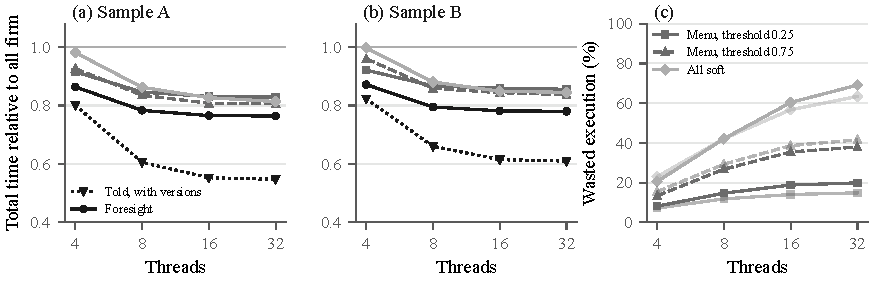
\includegraphics[width=\textwidth]{figures/fig_replay.pdf}
\caption{Replay in block order, by number of threads. (a) and (b) Total time relative to every declaration firm, in Sample A and Sample B. (c) Share of execution time wasted on aborted runs, with Sample B faded; foresight and Told abort nothing. Table~\ref{tab:replay} in Appendix~\ref{app:methods} gives the values, with free order.}
\label{fig:replay}
\end{figure*}

\begin{table*}[t]
\centering
\caption{What the classes buy and what a hold does, by setting, in pairs for Samples A and B.}
\label{tab:settings}
\footnotesize
\setlength{\tabcolsep}{2.5pt}
\begin{tabular}{@{}llllllll@{}}
\toprule
Setting & $r_o/\cp_o$ & Foresight & Told & \begin{tabular}{@{}l@{}}Classes\\from writes\end{tabular} & Menu & All soft & Hold: write; shared lock; soft; soft read (\%) \\
\midrule
Producer, 4 threads & 0.59, 0.61 (0.00, 0.00) & 0.90, 0.93 &  & 0.96, 0.97 & 0.96, 0.98 & 1.07, 1.09 & 7.3, 14; 6.3, 14; 22, 19; 22, 19 \\
Producer, 16 threads & 0.10, 0.07 (0.00, 0.00) & 0.71, 0.78 &  & 0.74, 0.80 & 0.78, 0.86 & 0.86, 0.91 & 19, 40; 16, 40; 1.6, 0.8; 1.6, 0.8 \\
Validator, 4 threads & 0.22, 0.18 (0.13, 0.11) & 0.86, 0.87 & 0.80, 0.82 & 0.89, 0.89 & 0.92, 0.92 & 0.98, 1.00 & 12, 25; 11, 25; 11, 23; 4.7, 8.8 \\
Validator, 16 threads & 0.07, 0.06 (0.27, 0.20) & 0.77, 0.78 & 0.55, 0.61 & 0.78, 0.80 & 0.83, 0.86 & 0.83, 0.85 & 25, 41; 24, 41; 23, 38; 0.2, 0.1 \\
\bottomrule
\end{tabular}
\par\smallskip\parbox{\textwidth}{\scriptsize A producer picks its order and is replayed in free order; a validator re-executes in block order and, outside the column Told, is not told what was written. Told: it is told what was written, and each run reads the version its place in the block requires; nothing runs twice. $r_o/\cp_o$: the cost of an unused soft declaration against an unused lock, with every declared account counted as read and, in parentheses, with only writes counted. Times are totals over the replayed blocks relative to every declaration firm; classes use the menu at $\theta = 0.25$. Hold: how much longer the other transactions take with one hold of the five hot accounts in each block, under the menu, by the class it declares. At a validator told what was written any hold adds only what its thread takes: 7.0, 12 at 4 threads and 0.2, 0.2 at 16.}
\end{table*}


\runin{Where the saving comes from}Applying the menu only to transactions that fail gives \freeFailedOnlyRatioSixteenA{} and \freeFailedOnlyRatioSixteenB{} of the all-firm time at a producer at 16 threads, and applying it only to those that succeed gives \freeOkOnlyRatioSixteenA{} and \freeOkOnlyRatioSixteenB{}, so nearly all of the saving is locks freed from transactions that fail; in the busiest minutes the two give \winFailedOnlyFreeMin{} to \winFailedOnlyFreeMax{} and \winOkOnlyFreeMin{} to \winOkOnlyFreeMax{}. It is concentrated: if only the 100 senders with the most unwritten lock time on hot accounts stopped holding what they do not write, a producer would get \harmTopHundredFreeA\% and \harmTopHundredFreeB\% of what classes from writes save and a validator \harmTopHundredBlockA\% and \harmTopHundredBlockB\%, and they send \topHundredTxA\% and \topHundredTxB\% of the replayed transactions. And it grows with a block's compute: on the quarter of blocks with the most compute the menu saves a producer \freeTopMenuCutSixteenA\% and \freeTopMenuCutSixteenB\%, against \freeRestMenuCutSixteenA\% and \freeRestMenuCutSixteenB\% on the rest, and likewise within \nTopAbove{} of the \nMinutes{} minutes. Across minutes the count of transactions says less: its rank correlation with the saving is \rankTpsFree{} at a producer and \rankTpsBlock{} at a validator.

\runin{The busiest minutes}We also replay the whole minutes of Section~\ref{sec:measure}, the first half of each estimating use (Table~\ref{tab:windows}). At 16 threads the menu saves \winFreeCutSixteenMin\% to \winFreeCutSixteenMax\% at a producer and \winBlockCutSixteenMin\% to \winBlockCutSixteenMax\% at a validator, and a validator told what was written saves \winToldSixteenMin\% to \winToldSixteenMax\%. At 4 threads a producer saves at most \winFreeCutFourMax\%, since reruns compete for too few threads.

\runin{At a producer}At 16 threads the menu saves \freeMenuLoCutSixteenA\% and \freeMenuLoCutSixteenB\% (95\% intervals from a bootstrap over blocks, \freeMenuLoCutCiLoSixteenA--\freeMenuLoCutCiHiSixteenA\% and \freeMenuLoCutCiLoSixteenB--\freeMenuLoCutCiHiSixteenB\%), wastes \freeMenuLoWasteSixteenA\% and \freeMenuLoWasteSixteenB\% of execution against \freeSoftWasteSixteenA\% and \freeSoftWasteSixteenB\% for all-soft, and beats it by \freeLeadSoftSixteenA{} and \freeLeadSoftSixteenB{} points of the all-firm time. At 4 threads, Agave's default for producing a block~\cite{agave}, it saves \freeMenuLoCutFourA\% and \freeMenuLoCutFourB\%, with intervals that include zero, and beats all-soft by \freeLeadSoftFourA{} and \freeLeadSoftFourB{} points. So from 8 threads up the menu is better than either single class, and at today's default and load it beats all-soft and ties all-firm. If every read-only declaration goes soft, a producer at 16 threads takes \softReadFreeRatioSixteenA{} and \softReadFreeRatioSixteenB{} of the all-firm time instead of \freeMenuLoRatioSixteenA{} and \freeMenuLoRatioSixteenB{}, so the read class costs it little.

\runin{At a validator}All-firm in block order is \firmBoundSixteenA{} and \firmBoundSixteenB{} times the bound set by total compute over threads at 16 threads, and more threads barely help past 8. The menu saves \menuLoCutSixteenA\% and \menuLoCutSixteenB\% (intervals \menuLoCutCiLoSixteenA--\menuLoCutCiHiSixteenA\% and \menuLoCutCiLoSixteenB--\menuLoCutCiHiSixteenB\%), and all-soft takes about the same time while wasting \softWasteSixteenA\% and \softWasteSixteenB\% of execution against \menuLoWasteSixteenA\% and \menuLoWasteSixteenB\%. Agave re-executes a block on a quarter of the machine's CPUs by default~\cite{agave}, so 16 threads mean 64 CPUs. A validator told what each transaction wrote needs no classes at all. With shared locks it runs on the foresight column, and if each run reads the version its place in the block requires it saves \toldCutSixteenA\% and \toldCutSixteenB\% at 16 threads and \toldCutFourA\% and \toldCutFourB\% at 4, wasting nothing. EIP-7928 has block producers publish these sets, and a block whose list is wrong is invalid~\cite{eip7928}. Classes therefore help the party that executes first, while the party that re-executes gains more from being told what was written.

\runin{What an unused soft declaration costs}We compare three runs with the same knowledge of what is written: what goes unwritten is held firm, held soft, or held only as a read. The cost of soft against the cost of firm, each relative to the third run, estimates $r_o/\cp_o$ (Table~\ref{tab:settings}). With only writes counted it is zero in free order by construction and \rOverCWritesFourB{} to \rOverCWritesSixteenA{} in block order. With every declared account counted as read it is \freeROverCSixteenA{} and \freeROverCSixteenB{} at a producer at 16 threads, \freeROverCFourA{} and \freeROverCFourB{} at 4 threads, and \rOverCSixteenA{} and \rOverCSixteenB{} at a validator. By Theorem~\ref{thm:floor} the second class lowers $r^\star_o$, and with it the trade-off, by this ratio. It is an average over ordinary declarations, and one long declaration costs more.

\begin{figure}[t]
\centering
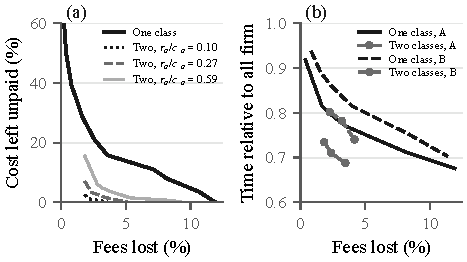
\includegraphics[width=\columnwidth]{figures/fig_frontier.pdf}
\caption{Theorem~\ref{thm:floor} on Solana traffic, with $x + \kappa$ three times what each transaction paid ($m = 3$). (a) Fees of successful transactions lost to reverts against the cost of unused declarations left unpaid, in Sample A; the one-class curve starts at 100\% unpaid. Each curve runs from no charge on an unused declaration to a charge of its full cost. (b) Time at a producer at 16 threads under the same choices; the two-class points use $r_o/\cp_o$ of that setting.}
\label{fig:frontier}
\end{figure}

\runin{The trade-off on Solana}Now let transactions respond. Take the price of an account to be the priority fee per unit of compute its writers paid in the first half, so an unused lock costs $\cp_o = p_o t$ at $\rho = 0$, and let $x + \kappa$ be $m$ times what the transaction paid. The fee is due whether it runs or reverts and it would not bid more than the trade is worth, so $m = 1$ is a lower bound; we lead with $m = 3$. Each declaration responds to its estimated use as a transaction that may use only that object would, with $k_o = \cp_o/3$, the stationary point above. Under one class a low fee cuts the unpaid cost fast, because most of what it drops is never used, but leaving nothing unpaid loses \frOneLostA\% and \frOneLostB\% of fees (Fig.~\ref{fig:frontier}(a)). Two classes get there at \frTwoLostA\% and \frTwoLostB\% with $r_o$ at a producer at 16 threads. With no charge on soft declarations they lose \frLeftLostA\% and \frLeftLostB\% and leave \frLeftUnpaidA\% and \frLeftUnpaidB\% unpaid, where one class that loses as much leaves \frOneAtLeftA\% and \frOneAtLeftB\%. A dropped account that a transaction only read would revert it as well, so these losses are lower bounds. On time, at equal fees lost two classes run \frGapFreeMin{} to \frGapFreeMax{} points faster at a producer (Fig.~\ref{fig:frontier}(b)) and \frGapBlockMin{} to \frGapBlockMax{} at a validator. At 16 threads the two-class curve stays inside the one-class curve at \frPointsInside{} of the \frPoints{} points we compare, across the samples, the minutes and the choices of Table~\ref{tab:frontier}. At a producer at 4 threads it need not, and where $r_o \ge \cp_o$ the two end at the same point, as Theorem~\ref{thm:floor} says.

\runin{Which price}These are the prices writers pay today, and they need a target near what an account uses. We let the price of~\eqref{eq:price} rise from today's price but not fall below it. With $U^\star_o$ at a quarter of the 20-million budget, counted use under the menu reaches it in \useClassAtQuarterA\% and \useClassAtQuarterB\% of hot block-account pairs and in at most \winClassUseAtQuarterMax\% in the busiest minutes, so on each minute's five hottest accounts the mean price stays within 5\% of today's price in \nPathNear{} of the \nMinutes{} minutes and averages \winPathFreeQuarterMax{} times it in the other, and fees on unused objects stay small under any rule. Only $\cp_o/(x+\kappa)$ matters to a drop, so $m = 30$ is the lead at a tenth of the price: one class then loses \frTabMThirtyOneEndA\% and \frTabMThirtyOneEndB\% and two \frTabMThirtyTwoEndA\% and \frTabMThirtyTwoEndB\%. The second class matters in proportion to the price a chain chooses to post.

\runin{What the fee adds}A producer could compute the menu's classes from public records with no fee and no declaration bit, so these times measure what classes are worth. But a sender can empty its record at no cost by switching to a new address: with no sender records the estimate falls back to the account alone, \freeAcctLoRatioSixteenA{} and \freeAcctLoRatioSixteenB{} of the all-firm time at a producer. A sender knows more than its record: classes from writes lead the menu by \freeLeadPerfectSixteenA{} and \freeLeadPerfectSixteenB{} points, a benchmark for what self-selection can add at fixed behavior. Unlike an estimate from public records, the fee also charges for a held lock.

\runin{Soft declarations last}A block rarely runs out of time: at a validator at 16 threads, of the \slAllBlocks{} blocks we replay, \slFirmOverBudget{} take as long as the 20-million-unit account budget read as time (Appendix~\ref{app:methods}) under all-firm and \slClassOverBudget{} under the menu. If a producer moves every transaction with a soft declaration behind the rest anyway, with outcomes held at their recorded values, the time at 16 threads goes from \slFreeRankA{} and \slFreeRankB{} of all-firm to \slFreeLastA{} and \slFreeLastB{}, so the saving does not rest on transactions with soft declarations keeping their rank.
\runin{What a hold costs}We add to each replayed block one transaction that runs for 1.4 million units of compute and declares the five accounts with the most declared compute in the first half of the sample, without writing them. Its place hardly matters: at a validator at 16 threads, from the head of the block to three quarters of the way through, the others take \placeBlockLoA\% to \placeBlockHiA\% longer in Sample A and \placeBlockLoB\% to \placeBlockHiB\% in Sample B, and the spread within a minute is at most \placeSpreadAll{} points. So the harm comes from the lock itself, and where the hold sits in the block barely matters. A shared lock delays others about as much as a write lock at a validator (Table~\ref{tab:settings}) and about as much or less at a producer, \winHoldFreeReadSixteenMed\% against \winHoldFreeFirmSixteenMed\% in the median busy minute. Under the rule both pay, with nothing back to the producer: \billWritersShareA\% and \billWritersShareB\% of a block's priority fees at the price writers pay on these accounts, and at the bids of the transactions around them, in the median block, \billLocalLoA\% to \billLocalHiA\% and \billLocalLoB\% to \billLocalHiB\%. Today it pays nothing per account. So the rule makes a hold cost what use costs and no more, and a manipulator who values the delay above this will pay. Declaring soft avoids the bill and gives up the lock: the others then take \holdFreeSoftSixteenA\% and \holdFreeSoftSixteenB\% longer at a producer at 16 threads and, with a soft read, \holdBlockSoftReadSixteenA\% and \holdBlockSoftReadSixteenB\% at a validator. A soft writable declaration still delays a validator not told what was written by \holdBlockSoftSixteenA\% and \holdBlockSoftSixteenB\%, and a validator told is delayed by \holdToldSixteenA\% and \holdToldSixteenB\% whatever is declared. At 4 threads a soft hold that keeps running again takes a thread, \holdFreeSoftFourA\% and \holdFreeSoftFourB\% at a producer. Over many blocks~\eqref{eq:hold} takes over: with $U^\star_o$ at a tenth of the budget the hold lifts the mean price on a minute's five hottest accounts to \winPathHoldTenthMed{} times today's price in the median busy minute, against \winPathFreeTenthMed{} with no hold.

\section{Reference implementation and a path to deployment}\label{sec:prototype}

\runin{What we built}We implemented the fee rules, the threshold choice, both counting rules and the damped premium, together with the scheduler used in Section~\ref{sec:replay}; \nTests{} unit tests cover the fee cases, lock and validation behavior and both orders of commit on random blocks. The rule runs in validators, so it has no contract and no gas table. It adds one bit per declared account to a transaction, a posted price and a posted premium per object, which the client does not keep today, and a constant-time fee computation per declared object. A chain that adopts object prices also has to burn the share of the usage fee that~\eqref{eq:shill} asks for; Solana today pays the whole priority fee to the validator~\cite{simd0096}.

\runin{Changes to a client}We mapped the changes onto Agave at a fixed commit~\cite{agave}. A v1 transaction's configuration would list the accounts it declares soft, writable or read-only, and older formats would stay all firm. An account declared soft takes no lock, and a commit-time check reruns a transaction if a transaction committed during its run wrote anything it read or wrote, in the manner of Block-STM's validation of read sets~\cite{gelashvili2023blockstm}; the replay, which cannot see reads, checks everything declared. The cost tracker would charge estimates to accounts declared firm only and actual costs to those and to accounts declared soft that are actually written. The fee adds $\cp_o$ for unused firm declarations and shared locks and $k_o$ for used soft declarations, and the rank's $C$ counts the lock costs of firm declarations. What the fee needs is close to hand at commit: the runtime records which write-locked accounts a transaction touched~\cite{agave}, which can only raise what a transaction pays, since that record is wider than a write.

\runin{A first step}The largest saving in our replay comes without any fee. If a block carries what each transaction wrote and validators keep an account's earlier version until its earlier readers have started, validators save the column Told of Table~\ref{tab:settings}, and a block whose list is wrong is invalid. An accounting change alone needs a feature gate (Solana's switch for activating a protocol change), the format field and posted prices, and no change to locks: a soft declaration keeps its write lock and leaves the account's budget until it is written. With classes as in Section~\ref{sec:replay} this frees \freedLoA\% and \freedLoB\% of the cost charged to the hot accounts, but an unused soft declaration then holds the lock for nothing and the budget no longer bounds the serial run on that account. A chain can begin with no fee on unused firm declarations and a large premium, where every transaction stays firm and the rule is today's, then raise the first and lower the second in steps, watching the serial run first and reruns once accounts declared soft give up their locks.

\runin{\artifactlink{Artifact}}The \artifactlink{anonymized artifact} holds the scripts that collect and reduce the public data, the aggregate outputs, the scripts behind every number, data table and data figure, the exact checks and the reference implementation. Raw samples, which contain account identifiers, are not included; the scripts refetch the samples and minutes by slot from public nodes while those slots are served.

\section{Conclusion}\label{sec:conclusion}

A chain that locks what transactions declare bears the cost of every declaration that goes unused. On Solana today most unused declarations come from transactions that fail, a few senders account for most of the waiting behind them, and a further lock adds nothing to what they pay. No single fee keeps declarations complete and charges for unused locks: any rule trades dropped declarations against unpaid cost, and how much depends on the cheapest way the chain offers to leave a declaration unused. A soft class that takes no lock lowers that cost. When an unused soft declaration costs nothing, one rule meets every goal, and under it a lock pays what use pays, on a write or a read.

\bibliographystyle{IEEEtran}
\bibliography{refs}

\appendices

\section{Ethics Considerations}\label{sec:ethics}

Every input to this paper is public: blocks and transaction metadata from public nodes, public source code and public documents. We sent no transaction to any chain, and the hold of Section~\ref{sec:replay} exists only in the simulator. We report aggregates only, with no account or sender named, and we do not attempt to identify the owners of accounts. Before submission we reported to the maintainers of the Agave and Firedancer clients and of Sui what Sections~\ref{sec:measure} and~\ref{sec:replay} find about their rules: who holds the accounts most in demand, what a hold costs others in replay and what it costs the holder. We sent them the rule of Section~\ref{sec:count} and the changes of Section~\ref{sec:prototype}, named no account or sender, and offered them the \artifactlink{artifact}. That a lock can be held at no charge was public already~\cite{simd0016}.

\section{Proofs}\label{app:proofs}

We checked the results of Sections~\ref{sec:oneclass}--\ref{sec:caps} by exact computation on finite instances, and their algebra symbolically; the scripts are part of the \artifactlink{artifact}.

\begin{proof}[Proof of Theorem~\ref{thm:menu} and Proposition~\ref{prop:class}]
We split the payoff of a complete declaration into a part its classes cannot affect and one cost per object. Write $\bar v(X)$ for $v(X)$ less the usage fees of the writable objects in $X$, and let $e_o$ be $(1-q_o)\cp_o$ for a firm declaration and $q_o k_o + (1-q_o) u_o$ for a soft one; a read-only object adds its charge, which does not depend on the branch. A complete declaration $\omega$ pays $\cp_o$ on the branches where $o$ is declared firm and unused, and $k_o$ or $u_o$ on the branches where $o$ is declared soft and used or unused, so
\begin{equation}\label{eq:split}
\Pi(\omega) = \mathbb{E}\,\bar v(X) - \sum_o e_o(\omega_o).
\end{equation}
The sum is minimized object by object, which gives the proposition. For the first claim of the theorem, against omitting $o$ a soft declaration gains $x_o + \kappa$ on the branches that use $o$ and costs $u_o$ on the others. For the rest, take $u_o = 0$, let $\omega$ omit a set $N$ that contains an object with $q_o > 0$, and let $\omega'$ declare the objects of $N$ soft. On a branch with $X \cap N = \emptyset$ the two pay the same, since an unused soft declaration pays nothing. On a branch that meets $N$, $\omega$ reverts and $\omega'$ runs, so
\begin{equation*}
\Pi(\omega') - \Pi(\omega) = \sum_{X \cap N \ne \emptyset} \Pr[X]\bigl(v(X) - \mathrm{fee}_{\omega'}(X) + \kappa\bigr) \ge 0,
\end{equation*}
because $\mathrm{fee}_{\omega'}(X) \le F(X) \le v(X) + \kappa$ for a type that can afford every branch. Some branch meets $N$ with positive probability, so positive margins make it strict.
\end{proof}

\begin{proof}[Proof of Lemma~\ref{prop:neutral}]
Part (a) reads off Definition~\ref{def:menu}, with $\pi \ge 1 \ge \sigma$ on a soft declaration and $\pi \ge \sigma\rho$ on a firm one. For (b), the producer earns $\gamma\pi p_o t + \gamma\sigma p_o t$ when the transaction takes $A$, since it can then resell $B$'s capacity, and $\gamma'\cp_o + \gamma\pi p_o t + \gamma_k k_o + \gamma\sigma\rho p_o t$ when it takes $B$. The difference is
\begin{equation*}
(1-\rho) p_o t (\gamma'\pi - \gamma\sigma) + \gamma_k k_o,
\end{equation*}
in which $\gamma'(1-\rho)\pi p_o t = \gamma'\cp_o$ and $\gamma_k k_o$ come from what the rule adds.
\end{proof}

\begin{proof}[Proof of Proposition~\ref{thm:shill}]
We follow Lemma~4 of~\cite{wadhwa2026perils} with a different count. A shill that adds $w$ to the count raises next block's price by $\eta p_o w/U^\star_o$, and use at the target in every later block keeps it there, so each of the $\Lambda$ blocks pays the producer $\gamma \eta \pi_o p_o w$ more. The shill itself pays at least $p_o w$, since every counted unit pays $\pi p_o$ with $\pi \ge 1$, and of this the producer gets back at most the share $\gamma$ of the usage fee. So its cost is at least $(1-\gamma) p_o w$, with equality for a used firm declaration at priority 1 and any size. A shill with $w = 0$ changes nothing. Comparing $(1-\gamma) p_o w$ with $\Lambda\gamma\eta\pi_o p_o w$ gives~\eqref{eq:shill}.
\end{proof}

\begin{proof}[Proof of Proposition~\ref{prop:premium}]
(a) We look for a root of $k - \Psi(k)$. Raising $k$ shrinks each declarer's soft range, so $s$ is nonincreasing, and it is continuous because $G$ has no atom on the boundary curves. So $\Psi$ is continuous and nonincreasing, $k - \Psi(k)$ is strictly increasing, it is at most zero at $k = 0$, and it grows without bound since $\Psi \le \Psi(0)$. (b) With uniform $q$ and $\cp = 1$, $s(k) = 1/(2(1+k)^2)$, so $\Psi(k) = 18/(1+k)^2$. The equation $k(1+k)^2 = 18$ factors as $(k-2)(k^2+4k+9) = 0$, and $\Psi'(2) = -36/27$, so iterates near $k^\star$ move away from it. (c) For $k > k'$, monotonicity and the Lipschitz bound give
\begin{equation*}
(1 - \delta - \delta\lambda)(k - k') \le f(k) - f(k') \le (1-\delta)(k - k')
\end{equation*}
for the damped map $f$. Its contraction factor is $\max\{1-\delta,\ |1-\delta(1+\lambda)|\} < 1$, and $f$ maps $[0,\infty)$ into itself since $\delta \le 1$.
\end{proof}

\begin{proof}[Proof of Proposition~\ref{prop:place}]
(a) At its rank the producer earns $\gamma\pi p_o t + \gamma_k k_o - k_o$ when the object is used and its resale $\gamma\sigma p_o t$ when it is not; last, the same without $k_o$ and with $q'$ in place of $q$. Subtracting gives the expression. (b) Firm at its rank gets $q(V + v(\emptyset)) + (1-q)(v(\emptyset) - \cp_o)$, and soft placed last gets $q'(V + v(\emptyset) - k_o) + (1-q')(v(\emptyset) - u_o)$. Subtracting, we get $(q - q')V + q' k_o + (1 - q')u_o - (1-q)\cp_o$.
\end{proof}

\begin{proof}[Proof of Proposition~\ref{prop:transfers}]
We count what leaves the party, since transfers cancel. A lock that goes unused or is read-only pays $(1-\rho)\pi' p_o t$, all burned, for $(1-\rho)t$ units of capacity, and a written object burns $(1-\gamma)\pi' p_o t$ of its usage fee for $t$ units, besides the premium $k_o$ of a soft declaration, which gives (a). For (b), on a branch with no revert the party gets $v(X)$ less $(1-\gamma)\sum_{o \in X \text{ writable}}\pi' p_o t$ and the burned charges, which include all that a read-only declaration pays, and on a revert it loses $(1-\gamma_{\mathrm{rev}})\kappa$; this is the payoff of the lone transaction. For (c), running a transaction with a soft declaration at its rank rather than last gains it $(q-q')(V - k_o + u_o)$, since a branch that uses $o$ is worth $V - k_o + u_o$ more to it than one that does not, and we add the producer's gain in Proposition~\ref{prop:place}(a) with $\gamma_k = 0$. A transfer splits the sum, so both can gain exactly when it is nonnegative.
\end{proof}

\begin{proof}[Proof of Proposition~\ref{prop:caps}]
If $p = \chi$ and $\xi = 1 - \rho$, then \eqref{eq:capS} and \eqref{eq:capU} coincide, and so do their maximizers. For the converse let $(p,\xi) \ne (\chi, 1-\rho)$. We build a need with two points on which the two objectives disagree. Let $Z = 1$ with probability $\beta$ and $Z = 2$ otherwise; limits other than $0, 1, 2$ are dominated. Moving the limit from 1 to 2 changes the objectives by
\begin{align*}
\Delta W &= v(1-\beta) - \chi(1-\rho) - \chi\rho(1-\beta),\\
\Delta \Pi &= v(1-\beta) - p\xi - p(1-\xi)(1-\beta),
\end{align*}
so $\Delta \Pi - \Delta W = (\chi - p) + \beta\bigl(p(1-\xi) - \chi\rho\bigr)$. This is affine in $\beta$ and not identically zero because $\chi > 0$, so it is nonzero for all $\beta$ close to 1. We choose $v$ so that $v(1-\beta)$ lies strictly between the two costs, and then $\Delta W$ and $\Delta \Pi$ have opposite signs. We also have to keep limit $0$ out of both. Unless $\xi = 0$ and $\rho = 1$, one of $\chi(1-\rho)$ and $p\xi$ is positive, so $v \to \infty$ as $\beta \to 1$, and running beats not running under both objectives. Otherwise $\xi = 0$ and $\rho = 1$, so $p \ne \chi$. Then $Z = 1$ with $v$ strictly between $\chi$ and $p$ makes the two objectives disagree.
\end{proof}

\section{Data and methods}\label{app:methods}

\runin{Solana}We read blocks from public RPC nodes, one block every 1,800 slots back from the finalized tip, and reduce each non-vote transaction to its format, sender, declared compute limit, consumed compute, cost units, fees, outcome, its writable accounts with signer, token, balance change and references, and its read-only accounts. The declared limit comes from the v1 configuration, else the compute-budget instruction, else the client's default of 3,000 per builtin instruction and 200,000 per other instruction, capped at 1.4 million. We exclude signers from the writable accounts counted: the fee payer's debit is itself a write, and other signers are left out with it. Estimating the probability of use on the first half of a sample and scoring it on the second gives a Brier score of \brierA{} and \brierB{}, against \brierBaseA{} and \brierBaseB{} for a constant base rate. A multi-hop route can write an intermediate account twice and leave its balance unchanged; counting a token account as unwritten only if no inner instruction received it gives \notWrittenStrictA\% and \notWrittenStrictB\%. An account counts as referenced only by a router's untaken leg if every top-level instruction that references it issued inner calls to a program other than the system, token, associated-token, compute-budget and memo programs and no inner instruction received the account.

\runin{Sui}We read transactions through the public GraphQL endpoint in October 2026, one checkpoint every 1,500 back from the latest and at most 50 transactions per checkpoint, and in November we reread the transactions whose inputs or object changes ran past the first page. A mutable shared input counts as unchanged at the upper bound if its contents are unchanged; at the middle estimate if also no object it directly owns changed; and at the lower bound if also no child object changed anywhere in the transaction. All \suiFailedMutable{} mutable declarations in failed transactions were unchanged.

\runin{Monad and Ethereum}On Monad we take \monadTx{} transactions from 150 blocks spaced 2,000 blocks apart and at most 12 per block. Public receipts record the limit as gas used, so we estimate need with \texttt{eth\_estimateGas} on the parent state, for the \monadEst{} transactions that return one. An estimate is an upper bound on need at that state and differs from need in the block's position, and \monadAboveLimit\% of estimates exceed the limit. On Ethereum we take \ethTx{} transactions from 40 blocks spaced 180 apart and compare \listsChecked{} access lists with the sets \texttt{eth\_createAccessList} returns on the parent state. These samples were collected in October 2026. The Sui storage fee of Section~\ref{sec:chains} comes from 40 checkpoints spaced 5,000 apart. In the October sample, \ethListShare\% of \ethTx{} Ethereum transactions carried a list, in line with the 1.46\% of Heimbach et al.~\cite{heimbach2025dissecting}. The set the node returns can leave out the sender, the recipient and precompiles, all warm already, and at the posted prices \listLoss\% of the lists lost gas. The parent state is not the transaction's position in its block, which overstates mismatches: re-executing the transactions of August 2023 with and without their lists, Heimbach et al.\ report that imperfect lists made almost 11.8\% of the transactions that carried one pay more than without it.

\runin{Avalanche}We take 600 evenly spaced blocks from the four weeks before the rule took effect and 600 from four weeks that start twelve days after, at most eight transactions per block, and keep calls seen at least three times in each window.

\runin{Other replay settings}The account budget of 20 million units bounds the compute of the transactions that write-lock one account in a slot~\cite{agave}; in those terms the all-firm time at 16 threads averages \firmMeanBudgetSixteenA\% and \firmMeanBudgetSixteenB\% of the budget and reaches \firmMaxBudgetSixteenA\% and \firmMaxBudgetSixteenB\% on the slowest block, and under the menu it averages \menuLoMeanBudgetSixteenA\% and \menuLoMeanBudgetSixteenB\%. A premium posted per account at three times the median compute of its declarers takes \freePostedRatioSixteenA{} and \freePostedRatioSixteenB{} of the all-firm time at a producer. Only \roWrittenA\% and \roWrittenB\% of read-only declarations sit on an account some transaction in the block wrote, so a charge on shared locks that follows write prices would fall on few of them. At a validator at 16 threads the menu is slower than all-firm in \menuLoSlowerSixteenA{} and \menuLoSlowerSixteenB{} of the \nBlocksHalf{} blocks. Ignoring reads of soft declarations, at a validator foresight saves \writesOracleCutSixteenA\% and \writesOracleCutSixteenB\%, the menu saves \writesMenuLoCutSixteenA\% and \writesMenuLoCutSixteenB\% with \writesMenuLoWasteSixteenA\% and \writesMenuLoWasteSixteenB\% wasted, and all-soft saves \writesSoftCutSixteenA\% and \writesSoftCutSixteenB\%, which brackets the reads we cannot see. Under the stricter count of writes the menu saves \strictMenuLoCutSixteenA\% and \strictMenuLoCutSixteenB\%. With behavior fixed at $\theta = 0.25$, $u_o = 0$ and one price and priority, the menu's charges come to $(1-\rho)$ times \incOverUsageA\% and \incOverUsageB\% of the usage fees on non-signer accounts, and \incOkFreeA\% and \incOkFreeB\% of successful transactions pay nothing beyond the usage fee.

\begin{table}[t]
\centering
\caption{Appendix table. Replay on the second half of each sample: total time relative to every declaration firm, with the percentage of execution wasted on aborted runs in parentheses. Every declared account counts as read, and foresight and a validator told what was written abort nothing. The first row of each group gives the all-firm time over the bound set by total compute over threads.}
\label{tab:replay}
\footnotesize
\setlength{\tabcolsep}{3pt}
\begin{tabular}{@{}lllll@{}}
\toprule
Threads & 4 & 8 & 16 & 32 \\
\midrule
\multicolumn{5}{@{}l}{\emph{Sample A, block order}} \\
All firm / bound & 1.35 & 2.35 & 4.62 & 9.22 \\
Foresight & 0.86 & 0.78 & 0.77 & 0.76 \\
Told, with versions & 0.80 & 0.61 & 0.55 & 0.55 \\
Menu, $\theta = 0.25$ & 0.92 (8) & 0.85 (15) & 0.83 (19) & 0.83 (20) \\
Menu, $\theta = 0.75$ & 0.93 (13) & 0.84 (27) & 0.81 (35) & 0.81 (38) \\
All soft & 0.98 (21) & 0.86 (42) & 0.83 (60) & 0.81 (69) \\
\midrule
\multicolumn{5}{@{}l}{\emph{Sample B, block order}} \\
All firm / bound & 1.45 & 2.68 & 5.31 & 10.61 \\
Foresight & 0.87 & 0.79 & 0.78 & 0.78 \\
Told, with versions & 0.82 & 0.66 & 0.61 & 0.61 \\
Menu, $\theta = 0.25$ & 0.92 (7) & 0.87 (12) & 0.86 (14) & 0.86 (15) \\
Menu, $\theta = 0.75$ & 0.96 (15) & 0.86 (29) & 0.84 (39) & 0.84 (42) \\
All soft & 1.00 (23) & 0.88 (42) & 0.85 (57) & 0.84 (63) \\
\midrule
\multicolumn{5}{@{}l}{\emph{Sample A, free order}} \\
All firm / bound & 1.20 & 1.86 & 3.49 & 6.92 \\
Foresight & 0.90 & 0.76 & 0.71 & 0.69 \\
Menu, $\theta = 0.25$ & 0.96 (6) & 0.85 (12) & 0.78 (18) & 0.75 (22) \\
Menu, $\theta = 0.75$ & 1.00 (11) & 0.89 (22) & 0.83 (34) & 0.80 (42) \\
All soft & 1.07 (18) & 0.97 (33) & 0.86 (45) & 0.80 (55) \\
\midrule
\multicolumn{5}{@{}l}{\emph{Sample B, free order}} \\
All firm / bound & 1.29 & 2.11 & 4.01 & 7.92 \\
Foresight & 0.93 & 0.83 & 0.78 & 0.77 \\
Menu, $\theta = 0.25$ & 0.98 (6) & 0.92 (10) & 0.86 (14) & 0.85 (16) \\
Menu, $\theta = 0.75$ & 1.04 (13) & 0.98 (26) & 0.91 (37) & 0.89 (43) \\
All soft & 1.09 (19) & 1.00 (32) & 0.91 (45) & 0.88 (53) \\
\bottomrule
\end{tabular}
\end{table}


\section{Further results}\label{app:more}

\begin{table}[t]
\centering
\caption{What is declared and what is used. Upper rows: share of declarations not written (Solana), not changed (Sui) or not in the set the node returned (Ethereum lists), with the stricter count for Solana and the range for Sui in parentheses. Solana includes failed transactions and Sui does not. Middle rows: aggregate use over the declared limit. Lower rows: the five accounts with the most declared compute in each block, Samples A and B.}
\label{tab:measure}
\scriptsize
\setlength{\tabcolsep}{2pt}
\begin{tabular}{@{}lll@{}}
\toprule
Chain & Declared & Share unused \\
\midrule
Solana, Sample A & 453{,}818 writable declarations & 57.1\% (56.3\%) \\
 & failed; token; route leg & 36.9; 17.8; 2.5\% \\
Solana, Sample B & 268{,}752 writable declarations & 57.9\% (56.9\%) \\
 & failed; token; route leg & 41.8; 12.0; 4.1\% \\
Sui & 5{,}501 mutable declarations & 50.3\% (12.7--53.3\%) \\
Ethereum lists & 1{,}679 addresses & 26.8\% \\
 & 7{,}323 storage keys & 32.0\% \\
\midrule
Chain & Declared & Use over limit \\
\midrule
Solana, Sample A & 46{,}150 compute limits & 0.25 \\
Solana, Sample B & 34{,}083 compute limits & 0.20 \\
Monad & 1{,}520 gas limits & 0.71 (estimated need) \\
Ethereum & 10{,}225 gas limits & 0.42 \\
\midrule
\multicolumn{2}{@{}l}{Hot lock time: writers; succeeded, not written} & 32, 39; 20, 21\% \\
\multicolumn{2}{@{}l}{\quad failed, sender succeeds at times; never} & 35, 18; 12, 21\% \\
\multicolumn{2}{@{}l}{Senders that never succeed: number; transactions} & 128, 128; 4{,}477, 4{,}491 \\
\multicolumn{2}{@{}l}{\quad share of declared hot compute} & 24, 23\% \\
\multicolumn{2}{@{}l}{Non-writers in cost charged, median pair} & 80.0, 68.2\% \\
\multicolumn{2}{@{}l}{Cost charged over the budget, median pair} & 12.3, 5.4\% \\
\multicolumn{2}{@{}l}{\quad pairs at half the budget, of 600} & 37, 12 \\
\multicolumn{2}{@{}l}{Holders' place in the block, median} & 0.53, 0.51 \\
\multicolumn{2}{@{}l}{Priority fee, writers; never (lamports per CU)} & 0.40, 0.65; 0.17, 0.19 \\
\bottomrule
\end{tabular}
\end{table}


\begin{table}[t]
\centering
\caption{Whole minutes of consecutive blocks: median (range) over the 11 busiest and the 4 at the median. Savings are against all firm. The slowest block is a share of the budget at a validator at 16 threads. Hold at 16 threads unless stated; its bill at the bids around it is the median over blocks. Tips: minutes recorded with them; at the median the top of the range is one transfer of 3.4 SOL. Top 100: their share of what foresight classes save. Fees: lost to leave nothing unpaid. Hot pairs: counted use under classes.}
\label{tab:windows}
\scriptsize
\setlength{\tabcolsep}{2pt}
\begin{tabular}{@{}lll@{}}
\toprule
 & Busiest & Median \\
\midrule
Non-vote transactions per second & 2102 (1764--3083) & 1221 (1219--1224) \\
Transactions that fail (\%) & 45 (35--74) & 29 (26--32) \\
Declarations unwritten (\%) & 65 (62--85) & 52 (48--56) \\
Hot lock time, writers (\%) & 32 (22--47) & 52 (42--58) \\
Hot lock time, failed (\%) & 58 (32--71) & 31 (17--35) \\
\quad sender writes it elsewhere (\%) & 31 (9--47) & 13 (9--20) \\
Classes, producer, 16 threads (\%) & 18 (5--30) & 16 (13--23) \\
Classes, producer, 4 threads (\%) & 1 ($-2$--9) & 4 (1--9) \\
Classes, validator, 16 threads (\%) & 22 (8--31) & 18 (17--20) \\
Classes, validator, 4 threads (\%) & 13 (4--21) & 9 (6--11) \\
Foresight, validator, 16 threads (\%) & 29 (16--39) & 26 (24--29) \\
Told, validator, 16 threads (\%) & 48 (30--56) & 41 (39--44) \\
Told, validator, 4 threads (\%) & 25 (17--33) & 17 (13--22) \\
$r_o/\cp_o$, producer, 16 threads & 0.11 ($-0.04$--0.33) & 0.14 (0.08--0.22) \\
$r_o/\cp_o$, validator, writes only & 0.25 (0.21--0.27) & 0.22 (0.21--0.24) \\
$r_o/\cp_o$, producer, 4 threads & 0.72 (0.15--1.77) & 0.51 (0.29--0.59) \\
Slowest block, all firm (\%) & 105 (50--147) & 102 (57--122) \\
Slowest block, classes (\%) & 82 (43--135) & 65 (49--86) \\
Slowest block, told (\%) & 79 (36--102) & 54 (25--77) \\
Hold, write lock, producer (\%) & 16 (2--41) & 26 (4--39) \\
Hold, soft, producer (\%) & 0.7 (0.1--1.2) & 0.8 (0.6--1.2) \\
Hold, soft, producer, 4 threads (\%) & 17 (7--24) & 20 (10--23) \\
Hold, told validator (\%) & 0.3 (0.2--0.6) & 0.5 (0.4--0.5) \\
Bill at writers' price, of block fees (\%) & 39 (16--91) & 70 (32--99) \\
Bill at bids around it, of block fees (\%) & 1.9 (0.2--16.1) & 4.2 (1.5--5.6) \\
Top 100, producer (\%) & 93 (38--95) & 93 (85--101) \\
Fees for none unpaid, one class (\%) & 13 (6--19) & 11 (6--15) \\
Fees for none unpaid, two classes (\%) & 4 (2--13) & 6 (2--6) \\
Tips over what is paid (\%) & 14.3 (7.7--26.7) & 18.2 (14.7--84.2) \\
Hot pairs at a tenth of the budget (\%) & 12.4 (0.0--34.8) & 10.5 (5.1--13.9) \\
\bottomrule
\end{tabular}
\end{table}


\begin{table}[t]
\centering
\caption{Fig.~\ref{fig:frontier} under other choices, in pairs for Samples A and B, with $r_o$ at a producer at 16 threads (\%).}
\label{tab:frontier}
\footnotesize
\setlength{\tabcolsep}{3pt}
\begin{tabular}{@{}lll@{}}
\toprule
Choice & \begin{tabular}{@{}l@{}}Fees lost for none\\unpaid: one; two\end{tabular} & \begin{tabular}{@{}l@{}}Two at $u_o = 0$: lost; unpaid;\\one at equal loss: unpaid\end{tabular} \\
\midrule
$m = 3$, the lead & 11.9, 11.4; 3.7, 4.3 & 1.8, 2.3; 2.5, 1.9; 27, 34 \\
$m = 1$ & 19.4, 18.4; 6.8, 9.3 & 4.6, 6.3; 1.0, 0.7; 16, 26 \\
$m = 10$ & 4.4, 5.3; 1.7, 1.6 & 0.6, 0.4; 5.2, 3.4; 42, 66 \\
$m = 30$ & 2.6, 2.4; 0.6, 0.9 & 0.1, 0.1; 7.1, 4.6; 70, 95 \\
$m = 100$ & 1.2, 1.2; 0.2, 0.4 & 0.0, 0.0; 7.8, 5.3; 90, 84 \\
One price & 6.2, 9.6; 2.6, 3.0 & 1.0, 1.4; 4.0, 2.1; 38, 43 \\
No smoothing & 14.5, 11.7; 6.8, 6.2 & 1.8, 2.1; 5.5, 4.2; 75, 64 \\
$k_o = 3\cp_o$ & 11.9, 11.4; 6.6, 8.6 & 6.0, 7.8; 0.2, 0.2; 13, 15 \\
\bottomrule
\end{tabular}
\end{table}


\runin{The trade-off under other choices}Table~\ref{tab:frontier} repeats the points of Fig.~\ref{fig:frontier}(a) with $m$ of 1, 10, 30 and 100, with the sample's overall price for every account, with the estimate of use without smoothing, and with $k_o = 3\cp_o$. In the busiest minutes where tips are recorded, counting them in what senders pay and in prices takes the fees lost to leave nothing unpaid from \winFrOneSameMin\% to \winFrOneSameMax\% to \winFrOneTipsMin\% to \winFrOneTipsMax\% with one class, and from \winFrTwoSameMin\% to \winFrTwoSameMax\% to \winFrTwoTipsMin\% to \winFrTwoTipsMax\% with two.

\runin{One fee at a uniform threshold}Let a fee on unused declarations make a transaction drop a declaration estimated to be used less often than $\tau = f_n/(f_n + x + \kappa)$ and lock the rest, and let a transaction that needs a dropped account revert. On the replay's estimate, $\tau = 0.05$ takes \freeOneFeeRatioLowSixteenA{} and \freeOneFeeRatioLowSixteenB{} of the all-firm time at a producer and \oneFeeRatioLowSixteenA{} and \oneFeeRatioLowSixteenB{} at a validator, at 16 threads. It drops \oneFeeDroppedLowA\% and \oneFeeDroppedLowB\% of declarations and makes \oneFeeRevertedLowA\% and \oneFeeRevertedLowB\% of successful transactions revert, which carry \oneFeeRevertedFeeLowA\% and \oneFeeRevertedFeeLowB\% of their priority fees. At $\tau = 0.25$ the times at a producer are \freeOneFeeRatioMidSixteenA{} and \freeOneFeeRatioMidSixteenB{} and the reverts \oneFeeRevertedMidA\% and \oneFeeRevertedMidB\%, carrying \oneFeeRevertedFeeMidA\% and \oneFeeRevertedFeeMidB\%. In the busiest minutes $\tau = 0.05$ takes \winOneFeeFreeMin{} to \winOneFeeFreeMax{} at a producer, with reverts of \winOneFeeRevertedMin\% to \winOneFeeRevertedMax\% carrying \winOneFeeRevertedFeeMin\% to \winOneFeeRevertedFeeMax\%.

\runin{Who would pay}If signers' use is counted too, the menu's charges come to $(1-\rho)$ times \incOverUsageSignersA\% and \incOverUsageSignersB\% of the usage fees. Of the \incSendersA{} and \incSendersB{} senders, the 100 with the largest charges pay \incTopHundredA\% and \incTopHundredB\% of the total. Failed transactions are \incFailedTxA\% and \incFailedTxB\% of the second half and pay \incFailedChargeA\% and \incFailedChargeB\% of the charges.

\runin{A hold under every firm declaration}With every declaration firm, at a validator at 16 threads, a hold of one account makes the others take \occFirmOneA\% and \occFirmOneB\% longer, of five \occFirmFiveA\% and \occFirmFiveB\%, and of twenty \occFirmTwentyA\% and \occFirmTwentyB\%.

\runin{Retrying under locks}A run that aborts could run again holding a lock on all it declared, so that no transaction runs more than twice. At a producer at 16 threads this cuts waste from \freeMenuLoWasteSixteenA\% and \freeMenuLoWasteSixteenB\% to \retryWasteA\% and \retryWasteB\%, raises the time from \freeMenuLoRatioSixteenA{} and \freeMenuLoRatioSixteenB{} of all-firm to \retryRatioA{} and \retryRatioB{}, and gives a soft hold its delay back, \retryHoldA\% and \retryHoldB\%, since the first collision hands it the lock. We keep the rerun without locks.

\runin{Budgets and limits}Before execution the compute declared on a hot account over a block reaches a median of \declLimMedA\% and \declLimMedB\% of the 20-million budget, and \declLimNinetyA{} and \declLimNinetyB{} times the budget at the 90th percentile, since estimates are replaced by actual costs as the block is built. The \defaultTxA\% and \defaultTxB\% of Solana transactions that set no limit carry \defaultDeclA\% and \defaultDeclB\% of the declared compute.

\runin{Limits and rank}The Solana Foundation notes that an excess request lowers a transaction's priority and that this, with the reservation, offsets the benefit of v1~\cite{natale2026resource}. Proposition~\ref{prop:caps} takes rank as given, so a chain with $\rho > 0$ has to settle that objection separately.

\end{document}
